% !TeX root = ../quantum.tex

\chapter{مبانی توزیع کلید کوانتومی (\lr{QKD})}
\label{chap:7}

\section*{چکیده}
این فصل به مبانی توزیع کلید کوانتومی (\lr{QKD}) اختصاص یافته است. فصل با توصیف تفاوت‌های کلیدی بین رمزنگاری متداول\LTRfootnote{Conventional cryptography}، امنیت لایه فیزیکی (\lr{PLS}) کلاسیک و \lr{QKD} آغاز می‌شود. در بخش مبانی \lr{QKD}، پس از یک مرور تاریخی، انواع مختلف \lr{QKD} را بررسی کرده و به‌اختصار مراحل معمول پس‌پردازش\LTRfootnote{Postprocessing}، یعنی مراحل مصالحه اطلاعات\LTRfootnote{Information reconciliation} و تقویت حریم خصوصی\LTRfootnote{Privacy amplification} را شرح می‌دهیم. در همان بخش، دو قضیه بنیادی را که \lr{QKD} بر آن‌ها استوار است ارائه می‌دهیم: قضیه کپی‌ناپذیری\LTRfootnote{No-cloning theorem} و قضیه عدم توانایی در تمایز ابهام‌ناپذیر حالت‌های کوانتومی غیرمتعامد\LTRfootnote{Non-orthogonal quantum states}. در بخش سیستم‌های \lr{QKD} با متغیر گسسته\LTRfootnote{Discrete variable (DV)} (\lr{DV-QKD})، پروتکل‌های \lr{BB84} و \lr{B92} و همچنین پروتکل‌های اکرت (\lr{E91}) و \lr{EPR} را به‌تفصیل توصیف می‌کنیم. در همان بخش، پروتکل کدگذاری فاز-زمان\LTRfootnote{Time-phase encoding} نیز شرح داده شده است. در رابطه با پروتکل‌های \lr{BB84}، نسخه‌های مختلف مناسب برای فناوری‌های گوناگون بررسی می‌شوند. در بخش امنیت \lr{QKD}، نرخ کلید مخفی\LTRfootnote{Secret-key rate (SKR)} (\lr{SKR}) به‌صورت حاصل‌ضرب نرخ کلید خام\LTRfootnote{Raw key rate} و نرخ کسری\LTRfootnote{Fractional rate} نمایش داده شده و به‌دنبال آن محدودیت‌های مختلف نرخ کلید خام توصیف می‌شوند. سپس، عبارت عمومی برای نرخ کسری ارائه شده و انواع استراتژی‌های شنود\LTRfootnote{Eavesdropping strategies}، شامل حملات انفرادی (مستقل یا غیرهمدوس)\LTRfootnote{Individual (independent or incoherent) attacks}، حملات دسته‌جمعی\LTRfootnote{Collective attacks}، حملات همدوس\LTRfootnote{Coherent attacks} و حملات هک کوانتومی/کانال جانبی\LTRfootnote{Quantum hacking/side-channel attacks} تشریح می‌گردند. برای حملات انفرادی و همدوس، عبارات کسر مخفی متناظر شرح داده شده‌اند. بخش بعدی به تعاریف مختلف امنیت، از جمله مفهوم $\epsilon$-امنیت\LTRfootnote{$\epsilon$-security} اختصاص یافته است. سپس، عبارات عمومی برای طرح‌های \lr{DV-QKD} دوبعدی برای هر دو پروتکل آماده‌سازی-و-اندازه‌گیری\LTRfootnote{Prepare-and-measure} و پروتکل‌های مبتنی بر حالت‌های فریب\LTRfootnote{Decoy states} استخراج می‌شوند. برای تسهیل توصیف پروتکل‌های \lr{QKD} با متغیر پیوسته\LTRfootnote{Continuous variable (CV)} (\lr{CV-QKD})، ابتدا مبانی اپتیک کوانتومی\LTRfootnote{Quantum optics} معرفی می‌شوند. در بخش پروتکل‌های \lr{CV-QKD}، هر دو نوع پروتکل مبتنی بر حالت‌های فشرده\LTRfootnote{Squeezed states} و حالت‌های همدوس\LTRfootnote{Coherent states} تشریح می‌شوند. با توجه به اینکه تولید و دست‌کاری حالت‌های همدوس بسیار ساده‌تر است، پروتکل‌های مبتنی بر حالت همدوس با هر دو نوع آشکارسازی هموداین و هتروداین\LTRfootnote{Homodyne and heterodyne detections} به‌تفصیل شرح داده شده‌اند. کسر مخفی برای هر دو پروتکل \lr{CV-QKD} مبتنی بر مصالحه مستقیم و معکوس استخراج شده است. علاوه بر این، جزئیات جنبه‌های کاربردی پروتکل \lr{GG02} ارائه شده و محاسبه کسر مخفی برای حملات دسته‌جمعی مورد بحث قرار گرفته است. سپس، مفاهیم پایه پروتکل‌های \lr{QKD} مستقل از دستگاه اندازه‌گیری\LTRfootnote{Measurement-device-independent (MDI)} (\lr{MDI-QKD}) معرفی می‌شوند. بخش پایانی ملاحظات پایانی مرتبط را ارائه می‌دهد.






\section{از رمزنگاری متداول تا \lr{QKD}}
\label{sec:7-1}

سیستم رمزنگاری\LTRfootnote{Cryptographic system} پایه مبتنی بر کلید در شکل \ref{fig:11-1} ارائه شده است. منبع، پیام (متن‌آشکار\LTRfootnote{Plaintext}) $M$ را به سمت بلوک رمزگذاری\LTRfootnote{Encryption} ارسال می‌کند که این بلوک با کمک کلید $K$ دریافت شده از منبع کلید، رمزنگاشت\LTRfootnote{Cryptogram} را تولید می‌نماید. در سمت گیرنده، رمزنگاشت ارسال شده از طریق کانال ناامن، توسط الگوریتم رمزگشایی\LTRfootnote{Decryption} به همراه کلید $K$ که از طریق کانال امن دریافت شده است، پردازش می‌شود که متن‌آشکار اصلی را برای تحویل به کاربر احرازهویت‌شده\LTRfootnote{Authenticated user} بازسازی می‌کند. فرآیند رمزگذاری را می‌توان به‌صورت ریاضی با $E_K(M) = C$ توصیف کرد، در حالی که فرآیند رمزگشایی با $D_K(C) = M$ بیان می‌شود. مشابه قبل، ترکیب توابع رمزگشایی و رمزگذاری منجر به نگاشت همانی\LTRfootnote{Identity mapping} $D_K(E_K(M)) = M$ می‌گردد. منبع کلید معمولاً کلید را به‌صورت تصادفی از فضای کلید\LTRfootnote{Keyspace} (محدوده مقادیر ممکن برای کلید) تولید می‌کند.

الگوریتم‌های مبتنی بر کلید را می‌توان به دو دسته کلی تقسیم کرد:
\begin{itemize}
	\item \textbf{الگوریتم‌های متقارن\LTRfootnote{Symmetric algorithms}:} که در آن‌ها کلید رمزگشایی را می‌توان از کلید رمزگذاری مشتق کرد و بالعکس. متناوباً، می‌توان از یک کلید یکسان برای هر دو مرحله رمزگذاری و رمزگشایی استفاده کرد. الگوریتم‌های متقارن با نام‌های الگوریتم‌های تک‌کلیدی\LTRfootnote{One-key (single-key) algorithms} یا کلید‌مخفی\LTRfootnote{Secret-key algorithms} نیز شناخته می‌شوند. سیستم شناخته‌شده‌ای که از این نوع الگوریتم استفاده می‌کند، استاندارد رمزگذاری دیجیتال\LTRfootnote{Digital encryption standard (DES)} (\lr{DES}) است \cite{7-1, 7-2, 7-3}.
	\item \textbf{الگوریتم‌های نامتقارن\LTRfootnote{Asymmetric algorithms}:} که در آن‌ها کلیدهای رمزگذاری و رمزگشایی متفاوت هستند. علاوه بر این، کلید رمزگشایی را نمی‌توان در یک بازه زمانی معقول از روی کلید رمزگذاری تعیین کرد. به دلیل این واقعیت، کلیدهای رمزگذاری حتی می‌توانند به‌صورت عمومی منتشر شوند، به‌طوری که یک شنودگر قادر به تعیین کلید رمزگشایی نباشد. سیستم‌های کلید عمومی\LTRfootnote{Public-key systems} \cite{7-4} بر پایه این مفهوم بنا شده‌اند. در سیستم‌های کلید عمومی، کلیدهای رمزگذاری به‌صورت عمومی منتشر می‌شوند، در حالی که کلید رمزگشایی تنها برای کاربر موردنظر شناخته شده است. در این حالت، کلید رمزگذاری را کلید عمومی\LTRfootnote{Public key} و کلید رمزگشایی را کلید مخفی (خصوصی)\LTRfootnote{Secret (private) key} می‌نامند. این کلیدها را می‌توان با هر ترتیبی برای ایجاد رمزنگاشت از متن‌آشکار و بازسازی متن‌آشکار از رمزنگاشت به کار برد.
\end{itemize}

\begin{figure}[H]
	\centering
	 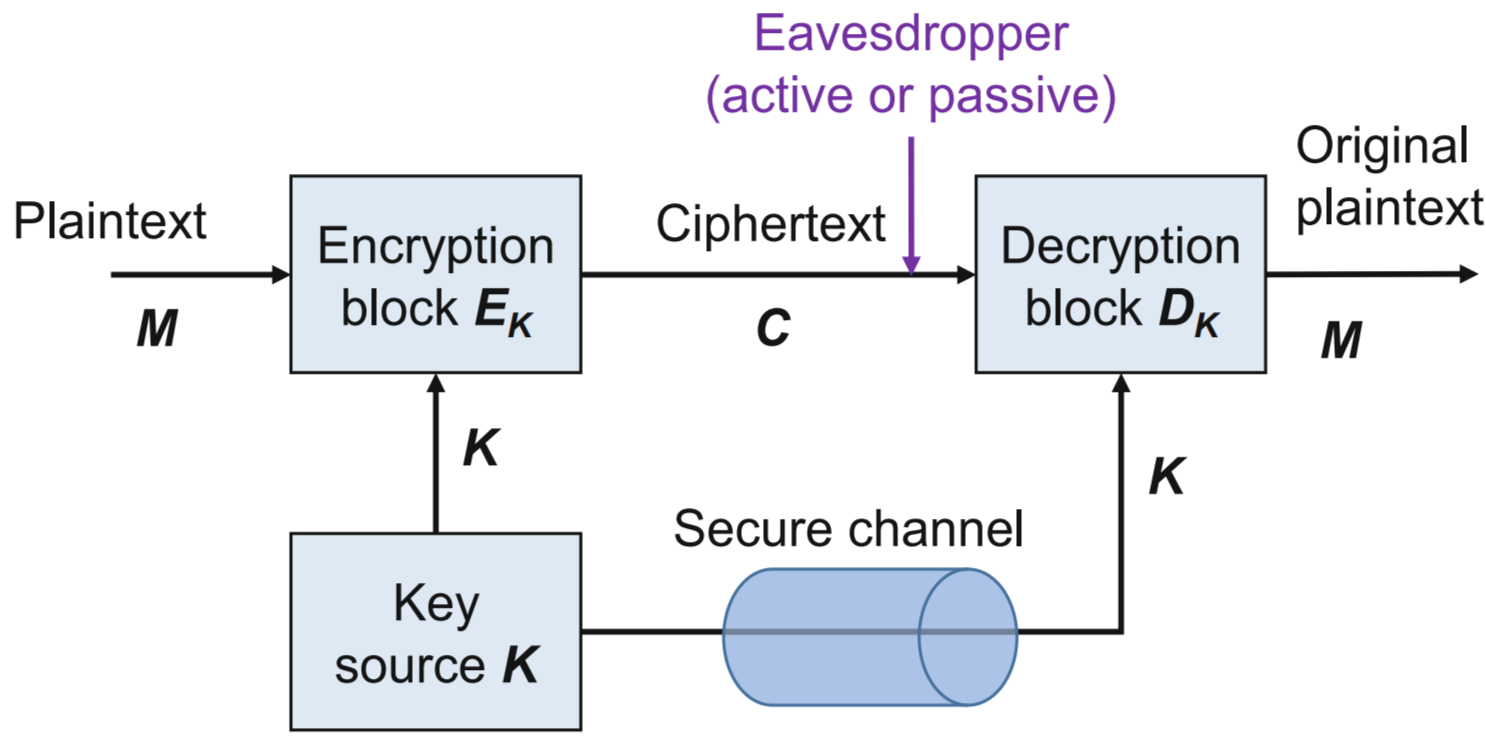
\includegraphics[width=0.7\textwidth]{chapters/figs/fig-7-1}
	\caption{طرح رمزنگاری پایه مبتنی بر کلید.}
	\label{fig:7-1}
\end{figure}






ساده‌ترین سیستم رمزنگاری کلید خصوصی، رمز ورنام\LTRfootnote{Vernam cipher} (پد یک‌بار مصرف\LTRfootnote{One-time pad}) است. در پد یک‌بار مصرف \cite{7-5}، یک دنباله کاملاً تصادفی از نویسه‌ها\LTRfootnote{Characters}، با طولی برابر با طول دنباله پیام، به‌عنوان کلید استفاده می‌شود. هنگامی که برای هر پیام جدید از یک دنباله تصادفی دیگر به‌عنوان کلید استفاده شود، طرح پد یک‌بار مصرف \textit{امنیت کامل}\LTRfootnote{Perfect security} را فراهم می‌کند که در فصل‌های \ref{chap:3} و \ref{chap:4} مورد بحث قرار گرفت. به بیان دقیق‌تر، رویکرد جستجوی جامع\LTRfootnote{Brute-force search} مستلزم بررسی $m^n$ کلید احتمالی است که در آن $m$ اندازه الفبای به‌کار رفته و $n$ طول رمزنگاشتِ شنود شده است. در عمل، در ارتباطات دیجیتال و کامپیوتری، ما معمولاً در الفبای باینری $\mathrm{GF}(2) = \{0, 1\}$ عمل می‌کنیم. برای به‌دست آوردن کلید، به یک مولد تصادفی خاص نیاز داریم و برای رمزگذاری با استفاده از طرح پد یک‌بار مصرف، صرفاً عمل جمع در پیمانه ۲، یعنی عملیات \lr{XOR}، را مطابق شکل \ref{fig:7-2} انجام می‌دهیم. اگرچه طرح پد یک‌بار مصرف امنیت کامل را ارائه می‌دهد، اما چندین نقص دارد \cite{7-6, 7-7, 7-8}: این طرح مستلزم توزیع امن کلید است، طول کلید باید حداقل به اندازه پیام باشد، بیت‌های کلید نمی‌توانند مجدداً استفاده شوند، کلیدها باید پیش از موعد تحویل داده شوند، تا زمان استفاده به‌صورت امن ذخیره گردند و پس از استفاده نابود شوند.

\begin{figure}[ht]
	\centering
	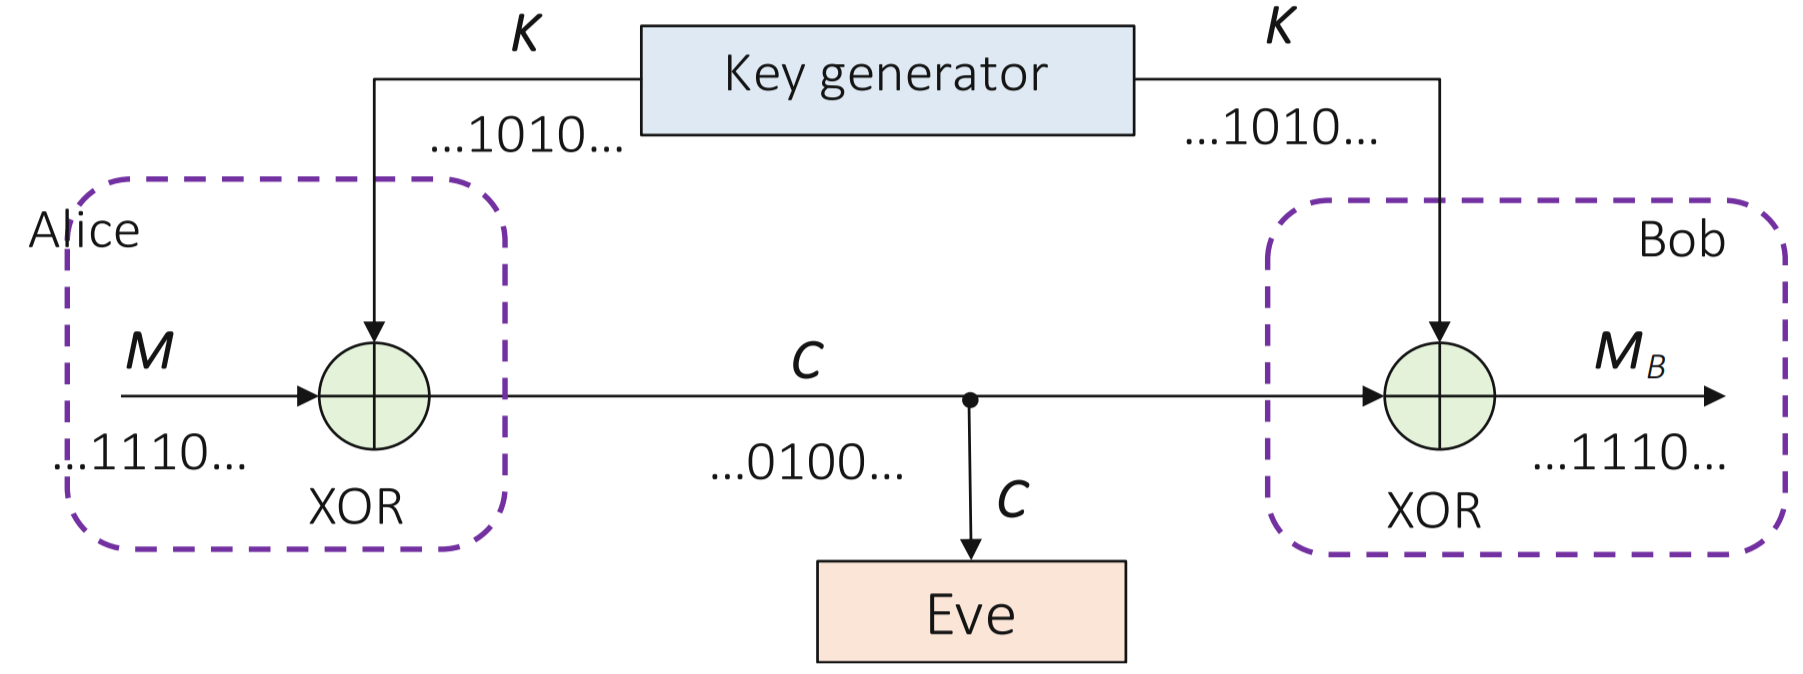
\includegraphics[width=0.8\textwidth]{chapters/figs/fig-7-2}
	\caption{طرح رمزگذاری پد یک‌بار مصرف.}
	\label{fig:7-2}
\end{figure}



طبق گفته شانون \cite{7-9}، امنیت کامل\LTRfootnote{Perfect security} که با نام امنیت غیرمشروط\LTRfootnote{Unconditional security} نیز شناخته می‌شود، زمانی حاصل می‌گردد که پیام‌های $\bm{M}$ و رمزنگاشت‌های $\bm{C}$ از نظر آماری مستقل باشند، به‌طوری که اطلاعات متقابل\LTRfootnote{Mutual information} متناظر برابر با صفر شود:
\begin{equation}
	I(\bm{M}, \bm{C}) = H(\bm{M}) - H(\bm{M}|\bm{C}) = 0 \Leftrightarrow H(\bm{M}|\bm{C}) = H(\bm{M})
	\label{eq:7-1}
\end{equation}
بنابراین، شرط محرمانگی کامل را می‌توان به‌صورت زیر خلاصه کرد:
\begin{equation}
	H(\bm{M}) \leq H(\bm{K}).
	\label{eq:7-2}
\end{equation}
به عبارت دیگر، برای اینکه یک طرح رمزگذاری از امنیت کامل برخوردار باشد، آنتروپی\LTRfootnote{Entropy} (عدم قطعیت\LTRfootnote{Uncertainty}) کلید نمی‌تواند کمتر از آنتروپی پیام باشد. با توجه به اینکه در رمز ورنام طول کلید حداقل برابر با طول پیام است، به نظر می‌رسد طرح پد یک‌بار مصرف دارای امنیت کامل باشد.

با این حال، از آنجا که برآورده کردن این شرط دشوار است، در رمزنگاری متداول به جای امنیت نظریه-اطلاعاتی\LTRfootnote{Information-theoretic security}، از امنیت محاسباتی\LTRfootnote{Computational security} استفاده می‌شود \cite{7-1, 7-3, 7-7, 7-10, 7-11, 7-12}. امنیت محاسباتی دو مورد تعدیل\LTRfootnote{Relaxation} را نسبت به امنیت نظریه-اطلاعاتی معرفی می‌کند \cite{7-3}:










\begin{itemize}
	\item امنیت در برابر یک شنودگر کارآمد\LTRfootnote{Efficient eavesdropper} که حملات تحلیل رمز\LTRfootnote{Cryptanalytic attacks} را برای مدت زمان مشخص و محدودی اجرا می‌کند، تضمین می‌شود. البته، در صورتی که شنودگر منابع محاسباتی کافی و/یا زمان کافی در اختیار داشته باشد، قادر خواهد بود امنیت طرح رمزگذاری را بشکند.
	\item شنودگران می‌توانند در شکستن پروتکل‌های امنیتی موفق شوند، اما با احتمال موفقیت ناچیز.
\end{itemize}
خواننده علاقه‌مند به یادگیری بیشتر درباره امنیت محاسباتی به کتاب ارزشمند کاتز\LTRfootnote{Katz} و لیندل\LTRfootnote{Lindell} \cite{7-3} ارجاع داده می‌شود. با این حال، با استفاده از محاسبات کوانتومی، هر طرح رمزنگاری متداول را می‌توان در بازه زمانی معقولی با به‌کارگیری الگوریتم تجزیه شور\LTRfootnote{Shor's factorization algorithm} \cite{7-13, 7-14, 7-15, 7-16, 7-17} شکست.

\section{مبانی \lr{QKD}}
\label{sec:7-2}
اخیراً دستاوردهای قابل‌توجهی در محاسبات کوانتومی حاصل شده است \cite{7-6, 7-7, 7-8}. بسیاری از شرکت‌ها در حال حاضر مشغول توسعه کامپیوترهای کوانتومی با مقیاس متوسط هستند. با توجه به اینکه اکثر سیستم‌های رمزنگاری به فرض دشواری محاسباتی\LTRfootnote{Computational hardness assumption} وابسته هستند، محاسبات کوانتومی چالشی جدی برای سیستم‌های امنیت سایبری\LTRfootnote{Cybersecurity} مدرن محسوب می‌شود. به‌عنوان یک مثال توصیفی، برای شکستن پروتکل ریواست-شامیر-ادلمن (\lr{RSA}) \cite{7-18}، همان‌طور که در فصل \ref{chap:3} بحث شد، باید دوره تناوب $r$ تابع $f(x) = m^x \pmod n = f(x+r)$ را تعیین کرد (به‌طوری که $r = 0, 1, \dots, 2^{l-1}$ و $m$ یک عدد صحیح کوچک‌تر از $n-1$ است). این دوره تناوب در یکی از مراحل الگوریتم تجزیه شور تعیین می‌شود \cite{7-6, 7-7, 7-8, 7-15, 7-16, 7-17}.








توزیع کلید کوانتومی (\lr{QKD}) با رمزگذاری متقارن را می‌توان به‌عنوان یکی از طرح‌های امنیت لایه فیزیکی\LTRfootnote{Physical-layer security} تفسیر کرد که می‌تواند امنیت اثبات‌پذیر\LTRfootnote{Provable security} را در برابر حملات آغاز شده توسط کامپیوترهای کوانتومی فراهم کند \cite{7-19}. نخستین طرح \lr{QKD} توسط بنت\LTRfootnote{Bennett} و براسارد\LTRfootnote{Brassard} معرفی شد که آن را در سال $1984$ پیشنهاد دادند \cite{7-13, 7-14} و امروزه با نام پروتکل \lr{BB84} شناخته می‌شود. امنیت \lr{QKD} توسط قوانین مکانیک کوانتومی\LTRfootnote{Quantum mechanics laws} تضمین می‌شود. درجات آزادی\LTRfootnote{Degrees of freedom (DOF)} مختلف فوتون، مانند قطبش، زمان، فرکانس، فاز و تکانه زاویه‌ای مداری\LTRfootnote{Orbital angular momentum (OAM)} (\lr{OAM}) را می‌توان برای پیاده‌سازی پروتکل‌های مختلف \lr{QKD} به کار گرفت. به‌طور کلی، بسته به استراتژی اعمال شده در سمت باب، دو طرح کلی \lr{QKD} وجود دارد: \lr{QKD} با متغیر گسسته\LTRfootnote{Discrete variable (DV)} (\lr{DV-QKD}) و \lr{QKD} با متغیر پیوسته\LTRfootnote{Continuous variable (CV)} (\lr{CV-QKD}). در طرح‌های \lr{DV-QKD}، یک آشکارساز تک‌فوتون\LTRfootnote{Single-photon detector (SPD)} (\lr{SPD}) در سمت باب به کار می‌رود، در حالی که در \lr{CV-QKD} مولفه‌های مربعی میدان\LTRfootnote{Field quadratures} با کمک آشکارسازی هموداین/هتروداین\LTRfootnote{Homodyne/heterodyne detection} اندازه‌گیری می‌شوند. طرح \lr{DV-QKD} با به‌کارگیری قضیه کپی‌ناپذیری و قضیه تمایزناپذیری حالت‌های کوانتومی دلخواه\LTRfootnote{Indistinguishability of arbitrary quantum states} به امنیت غیرمشروط\LTRfootnote{Unconditional security} دست می‌یابد که پیش‌تر در فصل \ref{chap:5} اثبات شده‌اند. قضیه کپی‌ناپذیری بیان می‌کند که حالت‌های کوانتومی دلخواه را نمی‌توان کپی کرد، که نشان می‌دهد ایو نمی‌تواند حالت‌های کوانتومی غیرمتعامد\LTRfootnote{Non-orthogonal states} را حتی با کمک کامپیوتر کوانتومی بازتولید کند. از سوی دیگر، قضیه دوم بیان می‌کند که حالت‌های غیرمتعامد را نمی‌توان به‌طور ابهام‌ناپذیر متمایز کرد. به‌ویژه، هنگامی که ایو با حالت‌های کوانتومی ارسالی تعامل برقرار می‌کند تا اطلاعاتی درباره بیت‌های ارسالی به‌دست آورد، به‌طور ناخواسته وفاداری\LTRfootnote{Fidelity} حالت‌های کوانتومی را مختل می‌کند که توسط باب شناسایی خواهد شد. از طرف دیگر، \lr{CV-QKD} از اصل عدم قطعیت\LTRfootnote{Uncertainty principle} بهره می‌برد که بیان می‌کند هر دو مولفه هم‌فاز\LTRfootnote{In-phase} و مربعی حالت‌های همدوس\LTRfootnote{Coherent states} را نمی‌توان به‌طور هم‌زمان با دقت کامل اندازه‌گیری کرد. ما همچنین می‌توانیم طرح‌های مختلف \lr{QKD} را به دو نوع «به کمک درهم‌تنیدگی»\LTRfootnote{Entanglement-assisted} یا «آماده‌سازی-و-اندازه‌گیری»\LTRfootnote{Prepare-and-measure} طبقه‌بندی کنیم.

پژوهش در \lr{QKD} در حال شتاب گرفتن است، به‌ویژه پس از اولین نمایش \lr{QKD} ماهواره به زمین\LTRfootnote{Satellite-to-ground} \cite{7-20}. اخیراً، \lr{QKD} در مسافت $404$ کیلومتری از فیبر نوری با تلفات بسیار کم\LTRfootnote{Ultralow-loss optical fiber} نمایش داده شده است؛ با این حال، این سیستم نرخ کلید امن بسیار پایینی ($3.2 \times 10^{-4}$ بیت بر ثانیه) داشت. با توجه به اینکه حالت‌های کوانتومی قابل تقویت نیستند، تضعیف فیبر مسافت را محدود می‌کند. از سوی دیگر، زمان مرده\LTRfootnote{Deadtime} (مدت زمانی که در آن یک \lr{SPD} به دلیل زمان بازیابی طولانی، نسبت به فوتون‌های ورودی پاسخگو نیست) در \lr{SPD}ها که معمولاً در محدوده $10$ تا $100$ نانوثانیه است، نرخ باود\LTRfootnote{Baud rate} و در نتیجه نرخ کلید امن را محدود می‌کند. طرح‌های \lr{CV-QKD}، از آنجا که از آشکارسازی هموداین/هتروداین استفاده می‌کنند، محدودیت زمان مرده ندارند؛ اما مسافت‌های معمول آن‌ها کوتاه‌تر است.

آلیس و باب با ارسال حالت‌های کیوبیت غیرمتعامد بین خود و بررسی اختلال در حالت ارسالی ناشی از کانال یا فعالیت ایو، می‌توانند حد بالایی برای نویز یا شنود در کانال ارتباطی کوانتومی خود تعیین کنند \cite{7-6}. آستانه حداکثر نرخ خطای تحمل‌پذیر\LTRfootnote{Maximum tolerable error rate} توسط بازدهی بهترین مراحل مصالحه اطلاعات\LTRfootnote{Information reconciliation} و تقویت حریم خصوصی\LTRfootnote{Privacy amplification} تعیین می‌شود \cite{7-6}.




\subsection{انواع سیستم‌های \lr{QKD}}
\label{subsec:7-2-1}
پروتکل‌های \lr{QKD} را می‌توان به چندین دسته کلی تقسیم کرد:
\begin{itemize}
	\item \textbf{\lr{QKD} وابسته به دستگاه\LTRfootnote{Device-dependent QKD}:} که در آن معمولاً منبع کوانتومی در سمت آلیس و آشکارساز کوانتومی در سمت باب قرار می‌گیرد. کلاس‌های محبوب آن عبارتند از: \lr{QKD} با متغیر گسسته (\lr{DV-QKD})، \lr{QKD} با متغیر پیوسته (\lr{CV-QKD})، \lr{QKD} به کمک درهم‌تنیدگی\LTRfootnote{Entanglement-assisted (EA) QKD} (\lr{EA-QKD}) و مرجع فاز توزیع‌شده\LTRfootnote{Distributed phase reference}. در \lr{EA-QKD}، منبع درهم‌تنیده را می‌توان در میانه کانال قرار داد تا مسافت ارسال افزایش یابد.
	\item \textbf{\lr{QKD} مستقل از دستگاه منبع\LTRfootnote{Source-device-independent QKD}:} که در آن منبع کوانتومی در سمت چارلی (ایو) قرار می‌گیرد، در حالی که آشکارسازهای کوانتومی در هر دو سمت آلیس و باب هستند.
	\item \textbf{\lr{QKD} مستقل از دستگاه اندازه‌گیری\LTRfootnote{Measurement-device-independent QKD (MDI-QKD)} (\lr{MDI-QKD}):} که در آن آشکارسازهای کوانتومی در سمت چارلی (ایو) قرار دارند، در حالی که منابع کوانتومی در هر دو سمت آلیس و باب مستقر هستند. حالت‌های کوانتومی در هر دو سمت آلیس و باب آماده‌سازی شده و به سمت آشکارسازهای چارلی ارسال می‌شوند. چارلی اندازه‌گیری‌های حالت بل\LTRfootnote{Bell state measurements} جزئی را انجام داده و زمانی که حالت بل جزئی مورد نظر شناسایی شد، آن را اعلام می‌کند؛ جزئیات مربوطه در ادامه ارائه خواهد شد.
\end{itemize}








\subsection{مراحل مصالحه اطلاعات و تقویت حریم خصوصی}
\label{sec:7-2-2}

مراحل پس‌پردازش کلاسیک\LTRfootnote{Classical postprocessing} در شکل \ref{fig:7-3} خلاصه شده است \cite{7-8}.

\begin{figure}[ht]
	\centering
	 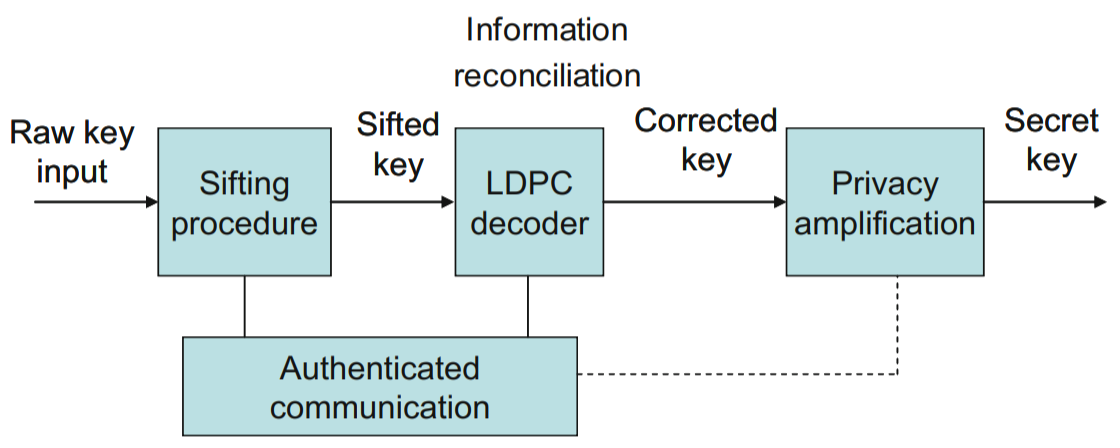
\includegraphics[width=0.8\textwidth]{chapters/figs/fig-7-3}
	\caption{مراحل پس‌پردازش کلاسیک.}
	\label{fig:7-3}
\end{figure}

کلید خام\LTRfootnote{Raw key} ناقص است و ما باید مراحل مصالحه اطلاعات\LTRfootnote{Information reconciliation} و تقویت حریم خصوصی\LTRfootnote{Privacy amplification} را انجام دهیم تا همبستگی بین رشته‌های دنباله $X$ (تولید شده توسط آلیس) و دنباله $Y$ (دریافت شده توسط باب) را افزایش دهیم و در عین حال، اطلاعات متقابل\LTRfootnote{Mutual information} شنودگر (ایو) درباره نتیجه را تا سطح امنیت مطلوب کاهش دهیم.

مصالحه اطلاعات چیزی جز تصحیح خطا\LTRfootnote{Error correction} نیست که روی یک کانال عمومی\LTRfootnote{Public channel} انجام می‌شود و خطاها را بین $X$ و $Y$ مصالحه می‌کند تا یک رشته بیت مشترک $K$ به‌دست آید، در حالی که اطلاعات فاش‌شده برای ایو تا حد امکان کمینه باشد.

تقویت حریم خصوصی \cite{7-21, 7-22} بین آلیس و باب برای استخراج\LTRfootnote{Distill} مجموعه کوچک‌تری از بیت‌ها $S$ از $K$ استفاده می‌شود که همبستگی آن با رشته ایو $Z$ زیر آستانه مطلوب باشد. یکی از راه‌های انجام تقویت حریم خصوصی، استفاده از توابع هش سراسری\LTRfootnote{Universal hash functions} $G$ است که مجموعه رشته‌های $n$-بیتی $A$ را به مجموعه رشته‌های $m$-بیتی $B$ نگاشت می‌کنند، به‌طوری که برای هر دو رشته متمایز $a_1, a_2 \in A$، وقتی $g$ به‌صورت یکنواخت و تصادفی از $G$ انتخاب شود، احتمال برقراری $g(a_1) = g(a_2)$ حداکثر $1/|B|$ باشد.











\subsubsection{قضیه کپی‌ناپذیری و تمایز حالت‌های کوانتومی}
\label{subsec:7-2-3}

\begin{theorem}
	\label{thm:7-1}
	\textit{قضیه کپی‌ناپذیری:} هیچ کپی‌کننده کوانتومی\LTRfootnote{Quantum copier} وجود ندارد که بتواند یک حالت کوانتومی دلخواه\LTRfootnote{Arbitrary quantum state} را کپی کند.
\end{theorem}

\begin{proof}
	اگر حالت ورودی $|\psi\rangle$ باشد، خروجی کپی‌کننده $|\psi\rangle|\psi\rangle$ خواهد بود. برای یک حالت کوانتومی دلخواه، وجود چنین کپی‌کننده‌ای منجر به یک تناقض بنیادی می‌شود.
	دو حالت دلخواه $|\psi\rangle$ و $|\chi\rangle$ را در نظر بگیرید که به‌عنوان ورودی به کپی‌کننده داده می‌شوند. هنگامی که این حالت‌ها به‌صورت مجزا وارد شوند، انتظار داریم خروجی‌های $|\psi\rangle|\psi\rangle$ و $|\chi\rangle|\chi\rangle$ را به‌دست آوریم. اکنون برهم‌نهی\LTRfootnote{Superposition} این دو حالت را به‌صورت زیر در نظر بگیرید:
	\begin{equation}
		\begin{aligned}
			|\phi\rangle = \alpha |\psi\rangle + \beta |\chi\rangle \implies |\phi\rangle |\phi\rangle &= (\alpha |\psi\rangle + \beta |\chi\rangle)(\alpha |\psi\rangle + \beta |\chi\rangle) \\
			&= \alpha^2 |\psi\rangle |\psi\rangle + \alpha\beta |\psi\rangle |\chi\rangle + \alpha\beta |\chi\rangle |\psi\rangle + \beta^2 |\chi\rangle |\chi\rangle
		\end{aligned}
		\label{eq:7-3}
	\end{equation}
	از سوی دیگر، خطی بودن\LTRfootnote{Linearity} مکانیک کوانتومی به ما می‌گوید که کپی‌کننده کوانتومی را می‌توان با یک عملگر یکانی\LTRfootnote{Unitary operator} نمایش داد که عمل کپی کردن را انجام می‌دهد. اگر چنین عملگر یکانی بر روی حالت برهم‌نهی $|\phi\rangle$ اثر کند، خروجی برهم‌نهیِ $|\psi\rangle|\psi\rangle$ و $|\chi\rangle|\chi\rangle$ خواهد بود؛ یعنی:
	\begin{equation}
		|\phi'\rangle = \alpha |\psi\rangle |\psi\rangle + \beta |\chi\rangle |\chi\rangle
		\label{eq:7-4}
	\end{equation}
	تفاوت بین دو معادله \eqref{eq:7-3} و \eqref{eq:7-4} منجر به تناقض ذکر شده در بالا می‌شود. در نتیجه، هیچ عملگر یکانی وجود ندارد که بتواند $|\phi\rangle$ را کپی کند.
\end{proof}

این نتیجه پرسش مرتبطی را ایجاد می‌کند: آیا حالت‌های خاصی وجود دارند که کپی کردن آن‌ها امکان‌پذیر باشد؟ پاسخ به این پرسش (به‌طور شگفت‌انگیزی) مثبت است. کپی کردن تنها برای حالت‌های متعامد متقابل\LTRfootnote{Mutually orthogonal states} امکان‌پذیر است.







\begin{theorem}
	\label{thm:7-2}
	تمایز ابهام‌ناپذیر\LTRfootnote{Unambiguously distinguish} حالت‌های کوانتومی غیرمتعامد\LTRfootnote{Non-orthogonal quantum states} غیرممکن است.
\end{theorem}

به عبارت دیگر، هیچ دستگاه اندازه‌گیری\LTRfootnote{Measurement device} نمی‌توان ساخت که بتواند با اطمینان حالت‌های غیرمتعامد را متمایز کند. این نتیجه بنیادی نقش مهمی در رمزنگاری کوانتومی\LTRfootnote{Quantum cryptography} ایفا می‌کند.

\begin{proof}
	\label{proof:7-2}
	اثبات آن بر پایه تناقض\LTRfootnote{Contradiction} است. فرض کنیم عملگر اندازه‌گیری $M$ یک عملگر هرمیتی\LTRfootnote{Hermitian operator} با مقادیر ویژه\LTRfootnote{Eigenvalues} $m_i$ و عملگرهای تصویر\LTRfootnote{Projection operators} $P_i$ متناظر باشد که به ما اجازه می‌دهد به‌طور ابهام‌ناپذیر بین دو حالت غیرمتعامد $|\psi_1\rangle$ و $|\psi_2\rangle$ تمایز قائل شویم. مقدار ویژه $m_1$ ($m_2$) به‌طور ابهام‌ناپذیر حالت $|\psi_1\rangle$ ($|\psi_2\rangle$) را شناسایی می‌کند. می‌دانیم که برای عملگرهای تصویر، ویژگی‌های زیر برقرار است:
	\begin{equation}
		\langle \psi_1 | P_1 | \psi_1 \rangle = 1, \quad \langle \psi_2 | P_2 | \psi_2 \rangle = 1, \quad \langle \psi_1 | P_2 | \psi_1 \rangle = 0, \quad \langle \psi_2 | P_1 | \psi_2 \rangle = 0.
		\label{eq:7-5}
	\end{equation}
	با توجه به اینکه $|\psi_2\rangle$ را می‌توان برحسب $|\psi_1\rangle$ و حالت دیگری مانند $|\chi\rangle$ که بر $|\psi_1\rangle$ متعامد\LTRfootnote{Orthogonal} است، به‌صورت زیر نمایش داد:
	\begin{equation}
		|\psi_2\rangle = \alpha |\psi_1\rangle + \beta |\chi\rangle.
		\label{eq:7-6}
	\end{equation}
	برای برقراری رابطه \eqref{eq:7-5}، $|\psi_2\rangle$ باید با $|\chi\rangle$ برابر باشد که نشان‌دهنده یک تناقض است.
\end{proof}






\section{پروتکل‌های توزیع کلید کوانتومی با متغیر گسسته (\lr{DV-QKD})}
\label{sec:7-3}
در این بخش، برخی از پروتکل‌های بسیار محبوب \lr{DV-QKD} را شرح می‌دهیم.

\subsection{پروتکل \lr{BB84}}
\label{subsec:7-3-1}
این پروتکل به نام بنت\LTRfootnote{Bennett} و براسارد\LTRfootnote{Brassard} نام‌گذاری شده است که آن را در سال $1984$ پیشنهاد دادند \cite{7-13, 7-14}. سه اصل کلیدی به‌کار گرفته شده عبارتند از: قضیه کپی‌ناپذیری، فروپاشی حالت\LTRfootnote{State collapse} در طول اندازه‌گیری، و بازگشت‌ناپذیری اندازه‌گیری‌ها\LTRfootnote{Irreversibility of measurements} \cite{7-6}. پروتکل \lr{BB84} را می‌توان با استفاده از درجات آزادی\LTRfootnote{Degrees of freedom (DOF)} (\lr{DOF}) مختلف، از جمله \lr{DOF} قطبش\LTRfootnote{Polarization DOF} \cite{7-23} یا فاز فوتون‌ها \cite{7-20} پیاده‌سازی کرد. از نظر تجربی، پروتکل \lr{BB84} در هر دو کانال فیبر نوری\LTRfootnote{Fiber-optics} و نوری فضای آزاد (\lr{FSO})\LTRfootnote{Free-space optical (FSO)} نمایش داده شده است \cite{7-23, 7-24}. پروتکل \lr{BB84} مبتنی بر قطبش در کانال فیبر نوری تحت تأثیر پاشندگی مد قطبشی\LTRfootnote{Polarization mode dispersion (PMD)}، تلفات وابسته به قطبش\LTRfootnote{Polarization-dependent loss (PDL)} و تلفات فیبر قرار می‌گیرد که مسافت ارسال را تحت تأثیر قرار می‌دهند. برای افزایش مسافت ارسال، در مرجع \cite{7-24} از کدگذاری فاز\LTRfootnote{Phase encoding} استفاده شده است. متأسفانه، نرخ کلید امن در $405$ کیلومتر فیبر با تلفات بسیار کم، بسیار ناچیز و تنها برابر با $6.5$ بیت بر ثانیه است. در یک کانال \lr{FSO}، اثرات قطبش به حداقل می‌رسد؛ با این حال، تلاطم اتمسفری می‌تواند منجر به اعوجاج جبهه‌موج\LTRfootnote{Wavefront distortion} و نوسانات فاز تصادفی شود. نمایش‌های قبلی \lr{QKD} شامل نمایش پیوند \lr{FSO} ماهواره به زمین\LTRfootnote{Satellite-to-ground} و نمایش روی یک پیوند \lr{FSO} بین دو نقطه در جزایر قناری\LTRfootnote{Canary Islands} بوده است \cite{7-23, 7-24}.

دو پایه‌ای که در پروتکل \lr{BB84} استفاده می‌شوند، پایه محاسباتی\LTRfootnote{Computational basis} $CB = \{ |0\rangle, |1\rangle \}$ و پایه قطری\LTRfootnote{Diagonal basis} هستند:
\begin{equation}
	DB = \left\{ |+\rangle = (|0\rangle + |1\rangle)/\sqrt{2}, \quad |-\rangle = (|0\rangle - |1\rangle)/\sqrt{2} \right\}.
	\label{eq:7-7}
\end{equation}
این پایه‌ها به دسته‌ای از پایه‌های متقابلاً بدون سوگیری\LTRfootnote{Mutually unbiased bases (MUBs)} (\lr{MUBs}) تعلق دارند \cite{7-25, 7-26, 7-27, 7-28, 7-29}. دو پایه متعامد\LTRfootnote{Orthonormal bases} $\{|e_1\rangle, \dots, |e_N\rangle\}$ و $\{|f_1\rangle, \dots, |f_N\rangle\}$ در فضای هیلبرت\LTRfootnote{Hilbert space} $\mathbb{C}^N$ زمانی \lr{MUB} هستند که مجذور اندازه ضرب داخلی\LTRfootnote{Inner product} بین هر دو حالت پایه $\{|e_m\rangle\}$ و $\{|f_n\rangle\}$ برابر با معکوس بُعد باشد:
\begin{equation}
	|\langle e_m | f_n \rangle|^2 = \frac{1}{N} \quad \forall m, n \in \{1, \dots, N\}.
	\label{eq:7-8}
\end{equation}
واژه کلیدی «بدون سوگیری»\LTRfootnote{Unbiased} بدین معناست که اگر سیستمی در حالتی متعلق به یکی از پایه‌ها آماده‌سازی شود، تمام نتایج اندازه‌گیری نسبت به پایه دیگر به یک اندازه محتمل هستند.

آلیس به‌طور تصادفی یک \lr{MUB} و به‌دنبال آن به‌طور تصادفی یک حالت پایه را انتخاب می‌کند. مقدار منطقی $0$ توسط حالت‌های $|0\rangle$ و $|+\rangle$، و مقدار منطقی $1$ توسط $|1\rangle$ و $|-\rangle$ بازنمایی می‌شود. باب هر کیوبیت را با انتخاب تصادفی پایه (محاسباتی یا قطری) اندازه‌گیری می‌کند. در فرآیند غربال‌گری\LTRfootnote{Sifting procedure}، آلیس و باب پایه‌های استفاده شده برای هر کیوبیت را اعلام کرده و تنها مواردی را نگه می‌دارند که در آن‌ها از پایه یکسانی استفاده کرده‌اند.






\subsubsection{پروتکل \lr{BB84}: توصیف رسمی}
\label{subsec:7-3-1-1}

آلیس دو دنباله تصادفی کلاسیک از بیت‌ها تولید می‌کند: دنباله داده $d$ و دنباله پایه‌ها $b$ که طول هر کدام $N > 4n$ است ($n$ طول کلید غربال‌شده است)، و آن‌ها را به‌صورت بلوکی از $N$ کیوبیت به شکل زیر کدگذاری می‌کند \cite{7-6}:
\begin{equation}
	\begin{aligned}
		|\bm{\psi}\rangle &= \bigotimes_{k=1}^N |\psi_{d_k b_k}\rangle \\
		|\psi_{00}\rangle &= |0\rangle, \quad |\psi_{10}\rangle = |1\rangle \\
		|\psi_{01}\rangle &= (|0\rangle + |1\rangle)/\sqrt{2}, \quad |\psi_{11}\rangle = (|0\rangle - |1\rangle)/\sqrt{2}
	\end{aligned}
	\label{eq:7-9}
\end{equation}
به‌وضوح، برخی از حالت‌ها نسبت به یکدیگر متعامد نیستند. اثر این فرآیند، کدگذاری دنباله بیت‌های داده $d$ در پایه \lr{DB} (پایه $X$) یا پایه \lr{CB} (پایه $Z$) بسته به دنباله پایه‌های $b$ است. باب حالت $\xi(|\bm{\psi}\rangle\langle\bm{\psi}|)$ را دریافت می‌کند که در آن $\xi$ یک عملگر کوانتومی\LTRfootnote{Quantum operation} برای توصیف اثر کانال کوانتومی و شنود است. باب هر کیوبیت دریافتی را در پایه \lr{CB} یا \lr{DB}، بسته به دنباله تصادفیِ پایه‌های $b'$ به طول $N$ که توسط خودش ایجاد شده است، اندازه‌گیری می‌کند تا نتایج اندازه‌گیری را که با $d'$ نشان داده می‌شود به‌دست آورد. آلیس $b$ را اعلام می‌کند و هر دو، تمام بیت‌های موجود در $\{d', d\}$ را به‌جز مواردی که بیت‌های متناظر در $b$ و $b'$ یکسان هستند، دور می‌ریزند. آلیس و باب $2n$ بیت را نگه می‌دارند. آلیس به‌طور تصادفی $n$ بیت از $2n$ بیت را انتخاب کرده و آن‌ها را اعلام می‌کند. باب و آلیس بیت‌های انتخاب‌شده را برای تخمین پارامتر\LTRfootnote{Parameter estimation} با هم مقایسه می‌کنند و اگر بیش از $t$ بیت اختلاف وجود داشته باشد (که متناظر با توانایی تصحیح خطای طرح تصحیح خطای پیشرو\LTRfootnote{Forward Error Correction (FEC)} (\lr{FEC}) است)، پروتکل را متوقف می‌کنند؛ در غیر این صورت، آن‌ها مراحل مصالحه اطلاعات و تقویت حریم خصوصی را انجام می‌دهند تا $m$ بیت کلید مشترک با محرمانگی قابل‌قبول را از $n$ بیت باقی‌مانده به‌دست آورند.









\subsubsection{مروری بر پروتکل BB84}
\label{subsec:7-3-1-2}
پروتکل \lr{BB84} را می‌توان به‌صورت زیر خلاصه کرد \cite{7-6}:
\begin{itemize}
	\item آلیس به‌طور تصادفی $N > 4n$ بیت داده تصادفی $d$ تولید می‌کند.
	\item آلیس به‌طور تصادفی یک دنباله از پایه‌های $b$ به طول $N$ بیت انتخاب کرده و $i$-امین بیت داده $d_i$ را به‌صورت $\{|0\rangle, |1\rangle\}$ (اگر بیت متناظر در $b$ برابر با $0$ باشد) یا $\{|+\rangle, |-\rangle\}$ (اگر بیت متناظر در $b$ برابر با $1$ باشد) کدگذاری می‌کند.
	\item حالت حاصل توسط آلیس برای باب ارسال می‌شود.
	\item به‌محض اینکه باب $N$ کیوبیت را دریافت کرد، این موضوع را اعلام نموده و هر کیوبیت را در یکی از پایه‌های \lr{CB} یا \lr{DB} که به‌طور تصادفی انتخاب شده‌اند، اندازه‌گیری می‌کند.
	\item آلیس دنباله پایه‌های $b$ مورد استفاده خود را اعلام می‌کند.
	\item آلیس و باب هر بیتی را که در آن از پایه‌های متفاوتی استفاده کرده‌اند، دور می‌ریزند. با احتمال بالا، حداقل $2n$ بیت باقی می‌ماند (در غیر این صورت پروتکل متوقف می‌شود) و آن‌ها از $2n$ بیت باقی‌مانده برای ادامه پروتکل استفاده می‌کنند.
	\item از میان $2n$ بیت باقی‌مانده، آلیس زیرمجموعه‌ای شامل $n$ بیت را جهت بررسی تداخل ایو و خطاهای کانال انتخاب کرده و به باب اطلاع می‌دهد که کدام بیت‌ها انتخاب شده‌اند.
	\item آلیس و باب مقادیر $n$ بیت استفاده شده برای تخمین نرخ خطای بیت کوانتومی\LTRfootnote{Quantum bit-error rate (QBER)} (\lr{QBER}) را اعلام و با هم مقایسه می‌کنند. اگر تعداد بیت‌های دارای اختلاف، بیش از مقدار قابل‌قبول (که توسط توانایی تصحیح خطای کد تعیین می‌شود) باشد، آن‌ها پروتکل را متوقف می‌کنند.
	\item در غیر این صورت، آلیس و باب مراحل مصالحه اطلاعات و تقویت حریم خصوصی را روی $n$ بیت باقی‌مانده انجام می‌دهند تا $m$ بیت کلید مشترک (که در آن $m < n$ است) به‌دست آورند.
\end{itemize}








\subsubsection{پروتکل \lr{QKD} \lr{BB84} مبتنی بر قطبش}
\label{subsec:7-3-1-3}
اکنون پروتکل \lr{QKD} \lr{BB84} مبتنی بر قطبش\LTRfootnote{Polarization-based} را با چهار حالت متناظر به‌کار رفته که در شکل \ref{fig:7-4} ارائه شده است، شرح می‌دهیم. پیاده‌سازی با قطعات اپتیکی حجیم\LTRfootnote{Bulky optics implementation} برای پروتکل \lr{BB84} در شکل \ref{fig:7-5} تصویر شده است.

\begin{figure}[ht]
	\centering
	 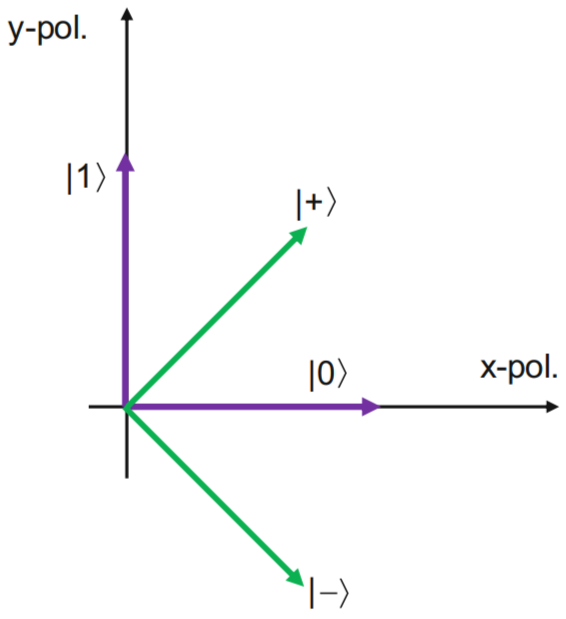
\includegraphics[width=0.4\textwidth]{chapters/figs/fig-7-4}
	\caption{چهار حالت به‌کار رفته در پروتکل \lr{BB84}.}
	\label{fig:7-4}
\end{figure}

\begin{figure}[ht]
	\centering
	 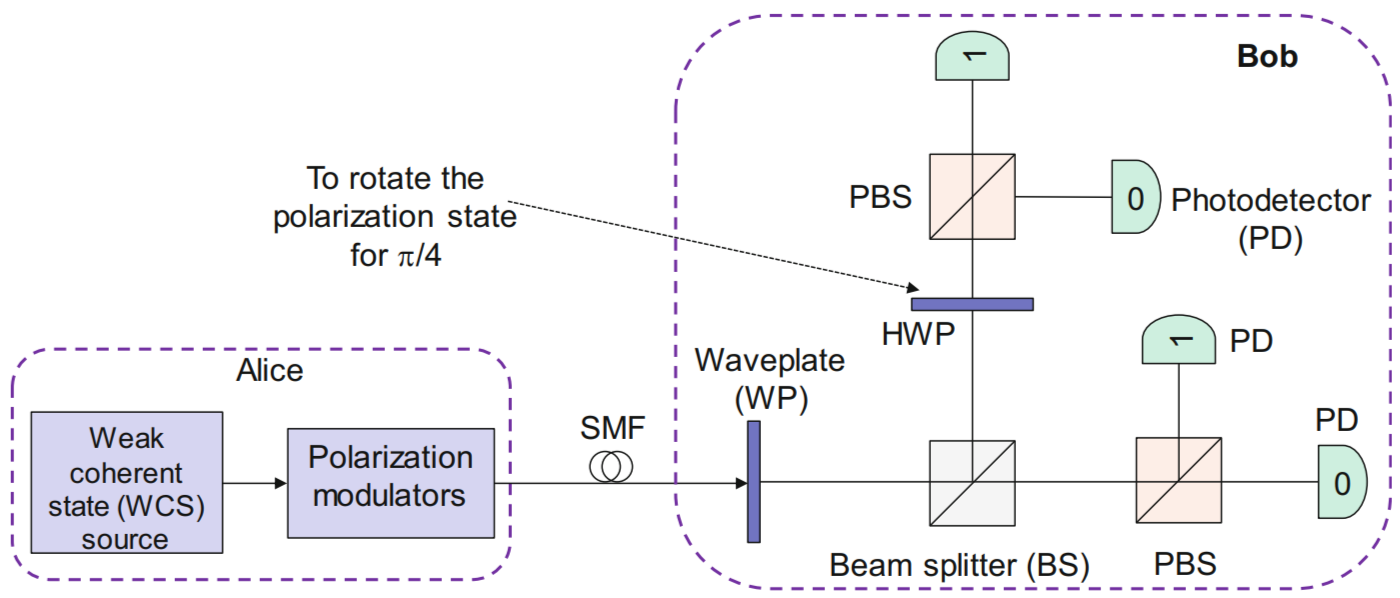
\includegraphics[width=0.9\textwidth]{chapters/figs/fig-7-5}
	\caption{پروتکل \lr{BB84} مبتنی بر قطبش.}
	\label{fig:7-5}
\end{figure}

حالت خروجی لیزر به‌عنوان حالت همدوس\LTRfootnote{Coherent state} شناخته می‌شود \cite{7-29, 7-30, 7-31, 7-32, 7-33, 7-34} که نشان‌دهنده کِت ویژه\LTRfootnote{Eigenket} راستِ عملگر نابودی\LTRfootnote{Annihilation operator} $a$ است؛ یعنی $a|\alpha\rangle = \alpha|\alpha\rangle$ که در آن $\alpha$ یک مقدار ویژه\LTRfootnote{Eigenvalue} مختلط است. بردار حالت همدوس $|\alpha\rangle$ را می‌توان برحسب کِت‌های ویژه متعامد پیش‌هنجار\LTRfootnote{Orthonormal eigenkets} $|n\rangle$ (حالت تعداد\LTRfootnote{Number state} یا حالت فوک\LTRfootnote{Fock state}) از عملگر تعداد\LTRfootnote{Number operator} $\hat{N} = a^\dagger a$ به‌صورت زیر نمایش داد:
\begin{equation}
	|\alpha\rangle = \exp[-|\alpha|^2/2] \sum_{n=0}^{+\infty} (n!)^{-1/2} \alpha^n |n\rangle
	\label{eq:7-10}
\end{equation}
حالت‌های همدوس متعامد نیستند، زیرا رابطه زیر برقرار است:







\begin{equation}
	\begin{aligned}
		|\langle\alpha | \beta\rangle|^2 &= \left| e^{-(|\alpha|^2+|\beta|^2)/2} \sum_{n=0}^{+\infty} \sum_{m=0}^{+\infty} (n!)^{-1/2}(m!)^{-1/2} \alpha^n (\beta^*)^m \langle n|m\rangle \right|^2 \\
		&= \left| e^{-(|\alpha|^2+|\beta|^2)/2} \sum_{n=0}^{+\infty} (n!)^{-1} \alpha^n (\beta^*)^n \right|^2 \\
		&= \left| e^{-(|\alpha|^2+|\beta|^2-2\alpha\beta^*)/2} \right|^2 = e^{-|\alpha-\beta|^2}.
	\end{aligned}
	\label{eq:7-11}
\end{equation}
زمانی که حالت همدوس به‌قدر کافی تضعیف شود، به حالت همدوس ضعیف\LTRfootnote{Weak coherent state} تبدیل می‌شود که می‌تواند تضمین کند حالت همدوس با احتمال بالایی بیش از یک فوتون نداشته باشد. به‌عنوان مثال، برای $0.1 = \alpha$ خواهیم داشت: $\dots + |2\rangle \sqrt{0.002} + |1\rangle \sqrt{0.09} + |0\rangle \sqrt{0.90} = |0.1\rangle$. حالت تعداد\LTRfootnote{Number state} $|n\rangle$ را می‌توان برحسب حالت پایه\LTRfootnote{Ground state} ($|0\rangle$) و با کمک عملگر تولید\LTRfootnote{Creation operator} به‌صورت زیر بیان کرد:
\begin{equation}
	|n\rangle = \frac{(a^\dagger)^n |0\rangle}{(n!)^{1/2}}.
	\label{eq:7-12}
\end{equation}
عملگر چگالی\LTRfootnote{Density operator} یک حالت همدوس به‌صورت زیر داده می‌شود:
\begin{equation}
	\rho = |\alpha\rangle\langle\alpha| = e^{-|\alpha|^2} \sum_{n=0}^{+\infty} \sum_{m=0}^{+\infty} (n!)^{-1/2}(m!)^{-1/2} \alpha^n (\alpha^*)^m |n\rangle\langle m|.
	\label{eq:7-13}
\end{equation}
جملات قطری $\rho$ به‌صورت زیر تعیین می‌شوند:
\begin{equation}
	\langle n | \rho | n \rangle = e^{-|\alpha|^2} \frac{|\alpha|^{2n}}{n!},
	\label{eq:7-14}
\end{equation}
که آشکارا یک توزیع پواسون\LTRfootnote{Poisson distribution} برای میانگین تعداد فوتون‌های $|\alpha|^2$ است. بنابراین، احتمال اینکه $n$ فوتون در حالت همدوس $|\alpha\rangle$ یافت شود، از توزیع پواسون پیروی می‌کند:
\begin{equation}
	P(n) = |\langle n | \alpha \rangle|^2 = e^{-\mu} \frac{\mu^n}{n!},
	\label{eq:7-15}
\end{equation}
که در آن از $\mu = |\alpha|^2$ برای نشان دادن میانگین تعداد فوتون‌ها استفاده شده است. با توجه به اینکه اکنون احتمال ارسال چندین فوتون غیرصفر است، ایو می‌تواند از این واقعیت برای کسب اطلاعات از کانال بهره‌برداری کند که با عنوان حمله تقسیم تعداد فوتون\LTRfootnote{Photon number splitting (PNS) attack} (\lr{PNS}) شناخته می‌شود. با فرض اینکه ایو قادر به تشخیص تعداد فوتون‌های رسیده به خود بدون انجام اندازه‌گیری روی سیستم باشد، زمانی که چندین فوتون شناسایی شوند، او یک تک‌فوتون را برداشته و آن را در حافظه کوانتومی\LTRfootnote{Quantum memory} قرار می‌دهد تا زمانی که آلیس و باب غربال‌گری زمانی و مصالحه پایه‌ها\LTRfootnote{Basis reconciliation} را انجام دهند. با یادگیری پایه‌های اندازه‌گیری آلیس و باب از طریق بحث در کانال عمومی احرازهویت‌شده، فوتون ذخیره‌شده در حافظه کوانتومی در پایه صحیح اندازه‌گیری شده و تمام اطلاعات موجود در فوتون در اختیار ایو قرار می‌گیرد.

برای غلبه بر حمله \lr{PNS}، استفاده از توزیع کلید کوانتومی مبتنی بر حالت فریب\LTRfootnote{Decoy state} در مرجع \cite{7-35} پیشنهاد شد. در \lr{QKD} حالت فریب، میانگین تعداد فوتون‌های ارسالی در بازه‌های زمانی تصادفی افزایش می‌یابد که به آلیس و باب اجازه می‌دهد تشخیص دهند آیا در زمان ارسال چندین فوتون، ایو در حال سرقت فوتون‌ها است یا خیر.











\subsubsection{\lr{QKD} \lr{BB84} مبتنی بر کدگذاری فاز}
\label{subsec:7-3-1-4}
اکنون پروتکل \lr{QKD} \lr{BB84} مبتنی بر کدگذاری فاز\LTRfootnote{Phase encoding} را شرح می‌دهیم که نسخه اپتیک حجیم\LTRfootnote{Bulky optics} آن در شکل \ref{fig:7-6} تصویر شده است.

\begin{figure}[ht]
	\centering
	 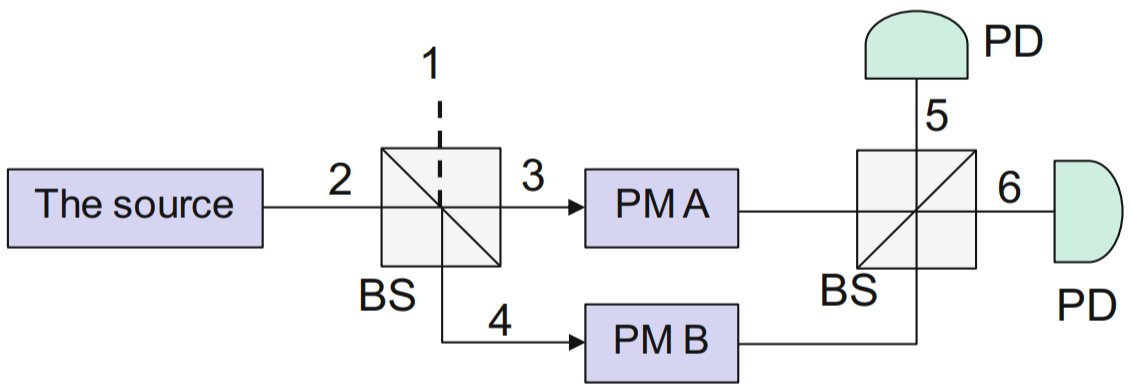
\includegraphics[width=0.8\textwidth]{chapters/figs/fig-7-6}
	\caption{پروتکل \lr{BB84} مبتنی بر کدگذاری فاز.}
	\label{fig:7-6}
\end{figure}

حالت پایه فوک\LTRfootnote{Fock basis} دو-مُدی ورودی $|01\rangle_{n_1 n_2}$ پس از اولین تقسیم‌کننده پرتو\LTRfootnote{Beam splitter} (\lr{BS}) به صورت زیر تبدیل می‌شود:
\begin{equation}
	|01\rangle_{n_1 n_2} \rightarrow 2^{-1/2}(j|01\rangle_{n_3 n_4} + |10\rangle_{n_3 n_4})
	\label{eq:7-16}
\end{equation}
پس از اعمال جابه‌جایی‌های فاز در شاخه‌های ماخ-زندر\LTRfootnote{Mach-Zehnder (MZ)} (\lr{MZ})، می‌توانیم بنویسیم:
\begin{equation}
	2^{-1/2}(j|01\rangle_{n_3 n_4} + |10\rangle_{n_3 n_4}) \rightarrow 2^{-1/2}(je^{-j\phi/2}|01\rangle_{n_3 n_4} + e^{j\phi/2}|10\rangle_{n_3 n_4}), \quad \phi = \phi_A - \phi_B
	\label{eq:7-17}
\end{equation}
که در آن $\phi_A$ ($\phi_B$) متناظر با جابه‌جایی فاز اعمال شده در شاخه بالایی (پایینی) متعلق به آلیس (باب) است. پس از \lr{BS} دوم، حالت متناظر به‌صورت زیر خواهد بود:
\begin{equation}
	|01\rangle_{n_3 n_4} \rightarrow 2^{-1/2}(j|01\rangle_{n_5 n_6} + |10\rangle_{n_5 n_6}), \quad |10\rangle_{n_3 n_4} \rightarrow 2^{-1/2}(j|10\rangle_{n_5 n_6} + |01\rangle_{n_5 n_6})
	\label{eq:7-18}
\end{equation}
حالت خروجی کلی را می‌توان به‌صورت زیر نمایش داد:
\begin{equation}
	|\psi(\phi)\rangle = j(\sin(\phi/2)|01\rangle_{n_5 n_6} + \cos(\phi/2)|10\rangle_{n_5 n_6})
	\label{eq:7-19}
\end{equation}
با تنظیم فازهای $\phi$ مختلف، می‌توانیم حالت‌های پروتکل \lr{BB84} را به‌صورت زیر تعریف کنیم:
\begin{equation}
	\begin{aligned}
		|\psi(0)\rangle &= j|10\rangle_{n_5 n_6} \doteq |0\rangle, \quad |\psi(\pi)\rangle = j|01\rangle_{n_5 n_6} \doteq |1\rangle \\
		|\psi(\pi/2)\rangle &= j2^{-1/2}(|10\rangle_{n_5 n_6} + |01\rangle_{n_5 n_6}) \doteq |+\rangle, \\
		|\psi(-\pi/2)\rangle &= j2^{-1/2}(|10\rangle_{n_5 n_6} - |01\rangle_{n_5 n_6}) \doteq |-\rangle
	\end{aligned}
	\label{eq:7-20}
\end{equation}
آلیس به‌طور تصادفی ولتاژ کنترل را برای اعمال جابه‌جایی فاز $\phi_A \in \{-\pi/2, 0, \pi/2, \pi\}$ تنظیم کرده و بنابراین به‌طور تصادفی حالت را انتخاب می‌کند. باب پایه اندازه‌گیری را با انتخاب تصادفی $\phi_B \in \{0, \pi/2\}$ برمی‌گزیند. اندازه‌گیری قاطع\LTRfootnote{Conclusive measurement} زمانی رخ می‌دهد که یا: (۱) $\phi_B = 0$ و $\phi_A \in \{0, \pi\}$ باشد و یا (۲) $\phi_B = \pi/2$ و $\phi_A \in \{-\pi/2, \pi/2\}$ باشد.













\subsection{پروتکل B92}
\label{subsec:7-3-2}
پروتکل \lr{B92} که در سال ۱۹۹۲ توسط بنت معرفی شد \cite{7-36}، تنها از دو حالت غیرمتعامد استفاده می‌کند، همان‌طور که در شکل \ref{fig:7-7} تصویر شده است. آلیس به‌طور تصادفی یک بیت کلاسیک $d$ تولید می‌کند و بسته به مقدار آن (۰ یا ۱)، حالت زیر را برای باب ارسال می‌نماید \cite{7-6}:
\begin{equation}
	|\psi\rangle = \begin{cases} 
		|0\rangle, & d = 0 \\ 
		|+\rangle = (|0\rangle + |1\rangle)/\sqrt{2}, & d = 1 
	\end{cases}
	\label{eq:7-21}
\end{equation}

\begin{figure}[ht]
	\centering
	% \includegraphics[width=0.6\textwidth]{fig7-7}
	\caption{دو حالت به‌کار رفته در پروتکل \lr{B92}.}
	\label{fig:7-7}
\end{figure}

باب به‌طور تصادفی یک بیت کلاسیک $d'$ تولید کرده و متعاقباً کیوبیت‌های دریافتی را در پایه محاسباتی\LTRfootnote{Computational basis} $CB = \{|0\rangle, |1\rangle\}$ (اگر $d'=0$) یا پایه قطری\LTRfootnote{Diagonal basis} $DB = \{|+\rangle, |-\rangle\}$ (اگر $d'=1$) اندازه‌گیری می‌کند؛ به‌طوری که نتیجه اندازه‌گیری $r=0$ یا ۱، متناظر با حالت‌های ویژه\LTRfootnote{Eigenstates} $1-$ و $1+$ از مشاهده‌پذیرهای\LTRfootnote{Observables} $X$ و $Z$ است که در جدول \ref{tab:7-1} نشان داده شده است. به‌وضوح، زمانی که نتیجه اندازه‌گیری $r=0$ باشد، حالت‌های احتمالی ارسال شده توسط آلیس $|0\rangle$ و $|+\rangle$ هستند و باب نمی‌داند آلیس کدام حالت را ارسال کرده است. از سوی دیگر، هنگامی که نتیجه اندازه‌گیری $r=1$ باشد، حالت‌های احتمالی آشکار شده توسط باب $|1\rangle$ و $|-\rangle$ هستند و بیت آشکار شده توسط باب متمم\LTRfootnote{Complement} بیت آلیس است.





\begin{table}[ht]
	\centering
	\caption{توضیح پروتکل \lr{B92}.}
	\label{tab:7-1}
	
	\small
	\begin{tabular}{|l|c|c|c|c|}
		\hline
		بیت‌های تولید شده توسط آلیس & \multicolumn{2}{c|}{$d = 0$} & \multicolumn{2}{c|}{$d = 1$} \\ \hline
		حالت‌های ارسال شده توسط آلیس & \multicolumn{2}{c|}{$|0\rangle$} & \multicolumn{2}{c|}{$|+\rangle$} \\ \hline
		بیت‌های تولید شده توسط باب & $d' = 0$ & $d' = 1$ & $d' = 0$ & $d' = 1$ \\ \hline
		پایه اندازه‌گیری باب & \lr{CB}: $\{|0\rangle, |1\rangle\}$ & \lr{DB}: $\{|+\rangle, |-\rangle\}$ & \lr{CB}: $\{|0\rangle, |1\rangle\}$ & \lr{DB}: $\{|+\rangle, |-\rangle\}$ \\ \hline
		\begin{tabular}[c]{@{}l@{}}حالت‌های حاصل احتمالی برای\\ آشکارسازی توسط باب\end{tabular} & $|0\rangle \quad |1\rangle$ & $|+\rangle \quad |-\rangle$ & $|0\rangle \quad |1\rangle$ & $|+\rangle \quad |-\rangle$ \\ \hline
		\begin{tabular}[c]{@{}l@{}}احتمال اندازه‌گیری یک\\ حالت معین توسط باب\end{tabular} & $1 \quad 0$ & $1/2 \quad 1/2$ & $1/2 \quad 1/2$ & $1 \quad 0$ \\ \hline
		نتیجه اندازه‌گیری باب $r$ & $0 \quad -$ & $0 \quad 1$ & $0 \quad 1$ & $0 \quad -$ \\ \hline
	\end{tabular}
\end{table}






باب به‌صورت عمومی مقدار $r$ را اعلام می‌کند (و البته $d'$ را مخفی نگه می‌دارد). آلیس و باب تنها آن جفت‌های $\{d, d'\}$ را نگه می‌دارند که برای آن‌ها نتیجه اندازه‌گیری $r=1$ بوده است. بیت نهایی کلید برای آلیس $d$ و برای باب $1-d'$ است. سپس مراحل مصالحه اطلاعات و تقویت حریم خصوصی انجام می‌شوند.








\subsection{پروتکل‌های اکرت (E91) و EPR}
\label{subsec:7-3-3}
پروتکل اکرت (\lr{E91})\LTRfootnote{Ekert (E91) protocol} در سال ۱۹۹۱ توسط اکرت معرفی شد \cite{7-37} (همچنین ببینید \cite{7-6}). فرض کنید آلیس و باب $n$ جفت‌کیوبیت درهم‌تنیده\LTRfootnote{Entangled} در حالت بل\LTRfootnote{Bell state} (جفت \lr{EPR}) $|B_{00}\rangle$ را به اشتراک می‌گذارند:
\begin{equation}
	|B_{00}\rangle = \frac{|00\rangle + |11\rangle}{\sqrt{2}}
	\label{eq:7-22}
\end{equation}
آلیس یک بیت کلاسیک تصادفی $b$ را برای تعیین پایه تولید کرده و نیمه خود از حالت بل را یا در پایه محاسباتی\LTRfootnote{Computational basis} $CB = \{|0\rangle, |1\rangle\}$ برای $b=0$ یا در پایه قطری\LTRfootnote{Diagonal basis} $DB = \{|+\rangle, |-\rangle\}$ برای $b=1$ اندازه‌گیری می‌کند تا بیت داده $d$ را به‌دست آورد. از سوی دیگر، باب به شیوه‌ای مشابه، به‌طور تصادفی بیت پایه $b'$ را تولید کرده و اندازه‌گیری را در یکی از پایه‌های \lr{CB} یا \lr{DB} انجام می‌دهد تا $d'$ را به‌دست آورد. آلیس و باب پایه‌های استفاده شده، یعنی $b$ و $b'$ را با هم مقایسه می‌کنند و تنها آن مواردی از $\{d, d'\}$ را برای کلید خام خود نگه می‌دارند که در آن‌ها پایه‌ها یکسان بوده است ($b=b'$). واضح است که کلید خام تولید شده به‌این صورت، کاملاً تصادفی است و تا زمانی که آلیس و باب اندازه‌گیری را روی نیمه‌های خود از حالت بل انجام ندهند، نامعین باقی می‌ماند. به همین دلیل، \lr{QKD} اساساً یک روش تولید کلید مخفی است، زیرا توسط منبع درهم‌تنیده تعیین می‌شود. اگر به جای آن، از حالت بل $|B_{01}\rangle = (|01\rangle + |10\rangle)/\sqrt{2}$ استفاده می‌شد، دنباله کلید خام باب متمم دنباله کلید خام آلیس می‌بود.

پروتکل \lr{EPR} یک پروتکل سه‌حالتی است که از نامساوی بل\LTRfootnote{Bell's inequality} برای تشخیص حضور ایو به‌عنوان یک متغیر تصادفی پنهان\LTRfootnote{Hidden random variable} استفاده می‌کند، همان‌طور که در مرجع \cite{7-38} توصیف شده است. فرض کنید $|\theta\rangle$ نشان‌دهنده حالت قطبش فوتونی باشد که به‌صورت خطی در زاویه $\theta$ قطبیده شده است. سه حالت قطبش ممکن برای جفت \lr{EPR} عبارتند از \cite{7-38}:
\begin{equation}
	\begin{aligned}
		|B_0\rangle &= \frac{|0\rangle|3\pi/6\rangle + |3\pi/6\rangle|0\rangle}{\sqrt{2}}, \\
		|B_1\rangle &= \frac{|\pi/6\rangle|4\pi/6\rangle + |4\pi/6\rangle|\pi/6\rangle}{\sqrt{2}}, \\
		|B_2\rangle &= \frac{|2\pi/6\rangle|5\pi/6\rangle + |5\pi/6\rangle|2\pi/6\rangle}{\sqrt{2}}
	\end{aligned}
	\label{eq:7-23}
\end{equation}
برای هر یک از این جفت‌های \lr{EPR}، قواعد کدگذاری زیر را اعمال می‌کنیم \cite{7-38}:
\begin{equation}
	|\psi\rangle_1 = \begin{cases} |0\rangle, & d=0 \\ |3\pi/6\rangle, & d=1 \end{cases}; \quad 
	|\psi\rangle_2 = \begin{cases} |\pi/6\rangle, & d=0 \\ |4\pi/6\rangle, & d=1 \end{cases}; \quad 
	|\psi\rangle_3 = \begin{cases} |2\pi/6\rangle, & d=0 \\ |5\pi/6\rangle, & d=1 \end{cases}
	\label{eq:7-24}
\end{equation}
عملگرهای اندازه‌گیری\LTRfootnote{Measurement operators} متناظر به‌صورت زیر خواهند بود \cite{7-38}:
\begin{equation}
	M_0 = |0\rangle\langle 0|, \quad M_1 = |\pi/6\rangle\langle \pi/6|, \quad M_2 = |2\pi/6\rangle\langle 2\pi/6|
	\label{eq:7-25}
\end{equation}
پروتکل \lr{EPR} را می‌توان اکنون به شرح زیر توصیف کرد. حالت \lr{EPR} یعنی $|B_i\rangle$ ($i=0,1,2$) به‌طور تصادفی انتخاب می‌شود. فوتون اول در جفت \lr{EPR} برای آلیس و فوتون دوم برای باب ارسال می‌شود. آلیس و باب به‌طور تصادفی، مستقل و با احتمال یکسان، یکی از عملگرهای اندازه‌گیری $M_0$، $M_1$ و $M_2$ را انتخاب می‌کنند. آن‌ها متعاقباً فوتون (کیوبیت) مربوط به خود را اندازه‌گیری می‌کنند و نتایج اندازه‌گیری، بیت متناظر برای کلید غربال‌شده\LTRfootnote{Sifted key} را تعیین می‌کند. به‌وضوح، انتخاب جفت‌های \lr{EPR} مطابق با رابطه \eqref{eq:7-23} منجر به کلیدهای خام متمم می‌شود. آلیس و باب سپس از طریق یک کانال عمومی احرازهویت‌شده با یکدیگر ارتباط برقرار می‌کنند تا مواردی را که در آن‌ها از عملگر اندازه‌گیری یکسانی استفاده کرده‌اند تعیین کنند و آن موارد را نگه می‌دارند. کلید مشترک حاصل، نشان‌دهنده کلید غربال‌شده است. مواردی که در آن‌ها از عملگرهای اندازه‌گیری متفاوتی استفاده کرده‌اند، نشان‌دهنده کلید ردشده\LTRfootnote{Rejected key} است و از این موارد برای تشخیص حضور ایو با به‌کارگیری نامساوی بل روی کلید ردشده استفاده می‌شود. آلیس و باب سپس مراحل مصالحه اطلاعات و تقویت حریم خصوصی را انجام می‌دهند.

اکنون به شرح این موضوع می‌پردازیم که چگونه کلید ردشده می‌تواند برای تشخیص حضور ایو مورد استفاده قرار گیرد \cite{7-38}. فرض کنید $P(\neq|i,j)$ نشان‌دهنده احتمال متفاوت بودن بیت‌های آلیس و باب در کلید ردشده باشد، با این فرض که عملگرهای اندازه‌گیری آلیس و باب به‌ترتیب یا $M_i$ و $M_j$ و یا $M_j$ و $M_i$ باشند. علاوه بر این، فرض کنید $P(=|i,j) = 1 - P(\neq|i,j)$ باشد. تفاضل بین این دو احتمال را با $\Delta P(i,j) = P(\neq|i,j) - P(=|i,j)$ نشان می‌دهیم. پارامتر بل\LTRfootnote{Bell's parameter} را می‌توان به‌صورت زیر تعریف کرد \cite{7-38}:
\begin{equation}
	\beta = 1 + \Delta P(1,2) - |\Delta P(0,1) - \Delta P(0,2)|
	\label{eq:7-26}
\end{equation}
که برای عملگرهای اندازه‌گیری فوق به $\beta \geq 0$ کاهش می‌یابد. با این حال، پیش‌بینی مکانیک کوانتومی مقدار $\beta = -1/2$ را به‌دست می‌دهد که به‌وضوح ناقض نامساوی بل است.












\subsection{کدگذاری فاز-زمان}
\label{subsec:7-3-4}
پروتکل \lr{BB84} علاوه بر حالت‌های قطبش، با استفاده از درجات آزادی\LTRfootnote{Degrees of freedom (DOF)} مختلفی مانند کدگذاری فاز-زمان\LTRfootnote{Time-phase encoding} \cite{7-39, 7-40, 7-41} و تکانه زاویه‌ای مداری\LTRfootnote{Orbital angular momentum} \cite{7-42, 7-43} نیز قابل پیاده‌سازی است. حالت‌های کدگذاری فاز-زمان برای پروتکل \lr{BB84} در شکل \ref{fig:7-8} ارائه شده‌اند که در مقایسه با شکل \ref{fig:7-6}، نسخه متفاوتی از طرح کدگذاری فاز محسوب می‌شود.

\begin{figure}[ht]
	\centering
	 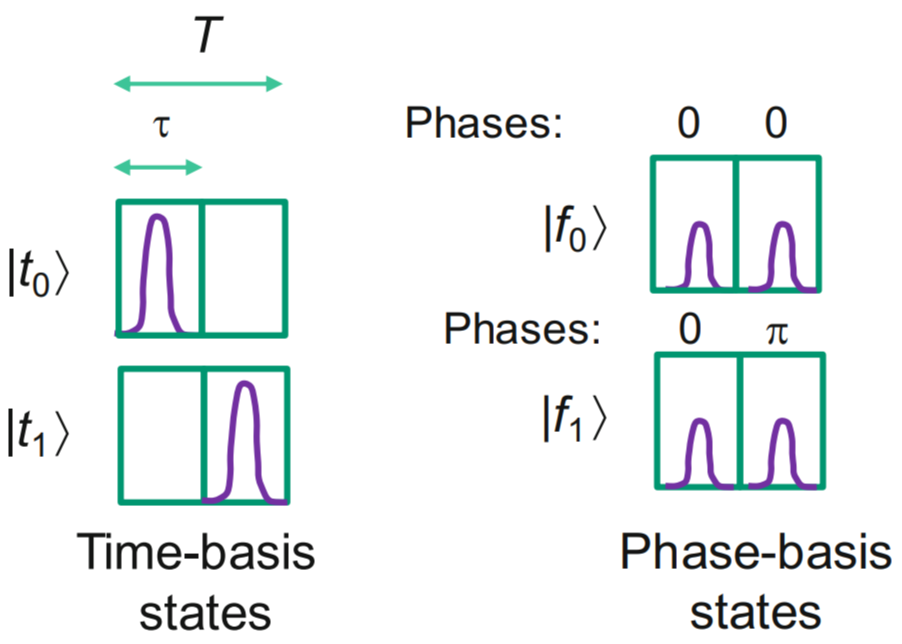
\includegraphics[width=0.7\textwidth]{chapters/figs/fig-7-8}
	\caption{حالت‌های کدگذاری فاز-زمان مورد استفاده در پروتکل \lr{BB84}.}
	\label{fig:7-8}
\end{figure}

پایه زمانی\LTRfootnote{Time basis} متناظر با پایه محاسباتی\LTRfootnote{Computational basis} و پایه فازی\LTRfootnote{Phase basis} متناظر با پایه قطری\LTRfootnote{Diagonal basis} است. پالس در یک بازه زمانی\LTRfootnote{Time bin} با مدت‌زمان $\tau = T/2$ متمرکز شده است. پایه زمانی مشابه مدولاسیون موقعیت پالس\LTRfootnote{Pulse-position modulation (PPM)} (\lr{PPM}) است. حالتی که در آن فوتون در اولین بازه زمانی قرار می‌گیرد با $|t_0\rangle$ و حالتی که در آن فوتون در دومین بازه زمانی قرار می‌گیرد با $|t_1\rangle$ نشان داده می‌شود. حالت‌های پایه‌های متقابلاً بدون سوگیری\LTRfootnote{Mutually unbiased bases (MUBs)} (\lr{MUB}) فازی به‌صورت زیر تعریف می‌شوند:
\begin{equation}
	|f_0\rangle = \frac{1}{\sqrt{2}} (|t_0\rangle + |t_1\rangle), \quad |f_1\rangle = \frac{1}{\sqrt{2}} (|t_0\rangle - |t_1\rangle).
	\label{eq:7-27}
\end{equation}

آلیس به‌طور تصادفی یا پایه زمانی و یا پایه فازی را انتخاب کرده و سپس به‌طور تصادفی یکی از حالت‌های پایه را برمی‌گزیند. مقدار منطقی $0$ توسط $|t_0\rangle$ و $|f_0\rangle$ و مقدار منطقی $1$ توسط $|t_1\rangle$ و $|f_1\rangle$ بازنمایی می‌شود. باب هر کیوبیت را با انتخاب تصادفی پایه، یعنی پایه زمانی یا فازی، اندازه‌گیری می‌کند. در فرآیند غربال‌گری\LTRfootnote{Sifting procedure}، آلیس و باب پایه‌های استفاده شده برای هر کیوبیت را اعلام کرده و تنها مواردی را که از پایه یکسانی استفاده کرده‌اند، نگه می‌دارند.

برای پیاده‌سازی رمزگذار فاز-زمان، می‌توان از مدولاتور قطبی الکترواپتیکی\LTRfootnote{Electro-optical polar modulator} (متشکل از اتصال پیاپی یک مدولاتور دامنه\LTRfootnote{Amplitude modulator} و یک مدولاتور فاز\LTRfootnote{Phase modulator}) یا مدولاتور \lr{I/Q} استفاده کرد \cite{7-44}. مدولاتور دامنه (مدولاتور ماخ-زندر\LTRfootnote{Mach-Zehnder modulator}) برای شکل‌دهی پالس و مدولاتور فاز برای اعمال جابه‌جایی فاز مطلوب به کار می‌روند، همان‌طور که در شکل \ref{fig:7-9} نشان داده شده است. از مولد شکل‌موج دلخواه\LTRfootnote{Arbitrary waveform generator (AWG)} (\lr{AWG}) برای تولید شکل‌موج‌های \lr{RF} متناظر بر حسب نیاز استفاده می‌شود. تضعیف‌کننده نوری متغیر\LTRfootnote{Variable optical attenuator (VOA)} (\lr{VOA}) نیز برای تضعیف باریکه مدوله‌شده تا سطح تک‌فوتون به کار می‌رود.



\begin{figure}[ht]
	\centering
	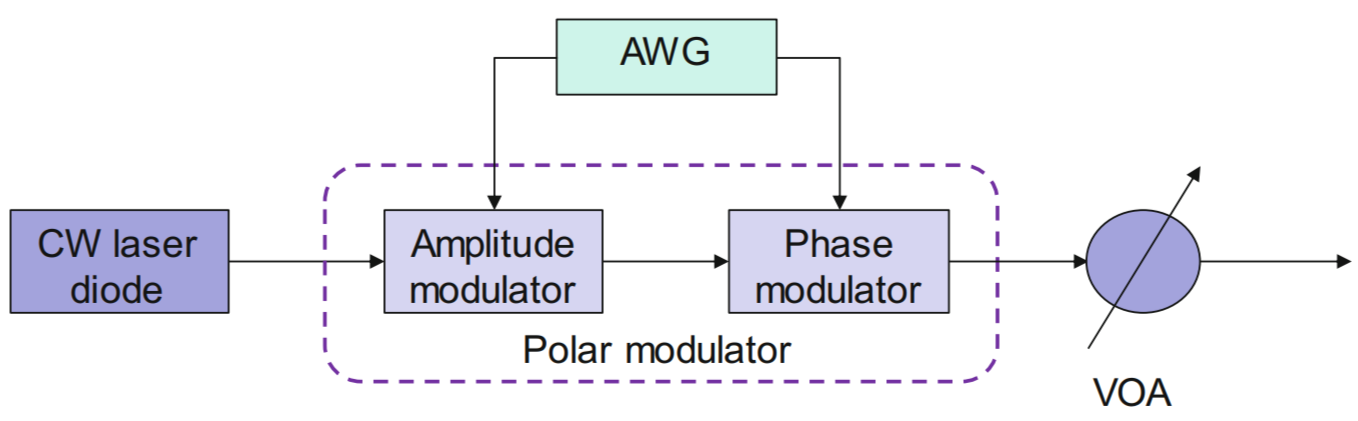
\includegraphics[width=0.8\textwidth]{chapters/figs/fig-7-9}
	\caption{رمزگذار فاز-زمان برای پروتکل \lr{QKD} \lr{BB84}. \lr{AWG}: مولد شکل‌موج دلخواه؛ \lr{VOA}: تضعیف‌کننده نوری متغیر.}
	\label{fig:7-9}
\end{figure}

در سمت گیرنده، حالت‌های پایه زمانی را می‌توان با کمک یک شمارنده تک‌فوتون\LTRfootnote{Single-photon counter} و مدارهای الکترونیکی مناسب آشکارسازی کرد. از سوی دیگر، برای آشکارسازی حالت‌های پایه فازی، می‌توان از یک تداخل‌سنج تأخیر-زمانی\LTRfootnote{Time-delay interferometer} استفاده کرد، همان‌طور که در مرجع \cite{7-45} توصیف شده است (شکل \ref{fig:7-10} را ببینید). اختلاف مسیر بین دو بازو برابر است با $\Delta L = \Delta L_0 + \delta L$ \cite{7-45}، که در آن $\Delta L_0$ اختلاف مسیری برابر با $c\tau$ ($c$ سرعت نور است) و $\delta L \ll \Delta L_0$ اختلاف مسیر اندکی است که برای تنظیم فاز استفاده می‌شود، زیرا $\phi = k\delta L$ ($k$ عدد موج\LTRfootnote{Wave number} است). هنگامی که حالت فازی $|f_0\rangle$ به رمزگشای فاز-زمان وارد می‌شود، خروجی‌های دومین تقسیم‌کننده پرتو\LTRfootnote{Beam splitter (BS)} (\lr{BS}) ۵۰:۵۰ سه بازه زمانی را اشغال می‌کنند. خروجی $+$ موردی را نشان می‌دهد که در آن خروجی‌های تداخل‌سنج تداخل سازنده\LTRfootnote{Constructive interference} دارند، در حالی که خروجی $-$ نشان‌دهنده تداخل ویرانگر\LTRfootnote{Destructive interference} خروجی‌های متناظر تداخل‌سنج است. برای تداخل سازنده، پالس میانی دوبرابر می‌شود، در حالی که برای تداخل ویرانگر، پالس‌های میانی یکدیگر را خنثی می‌کنند. بنابراین، کلیک آشکارساز تک‌فوتون\LTRfootnote{Single-photon detector (SPD)} (\lr{SPD}) در بازه میانی در خروجی $+$، حالت $|f_0\rangle$ را شناسایی می‌کند، در حالی که کلیک متناظر در خروجی $-$، حالت $|f_1\rangle$ را تشخیص می‌دهد.



\begin{figure}[ht]
	\centering
	 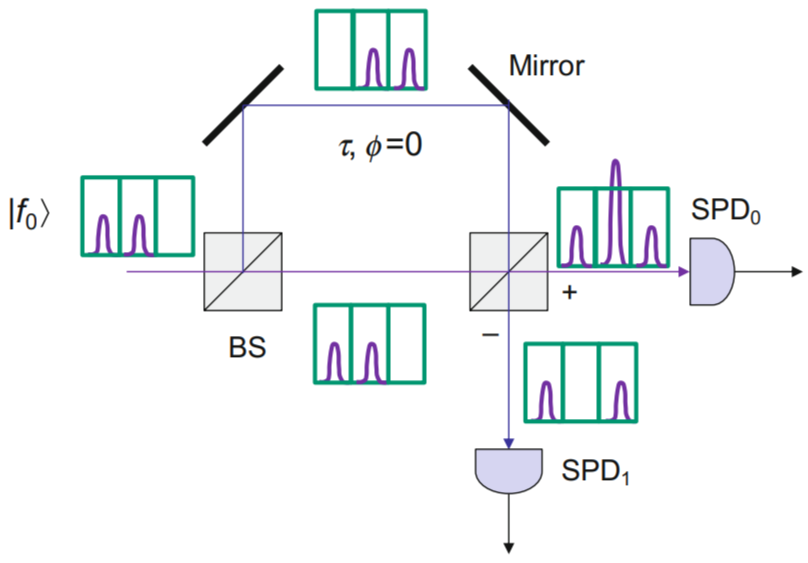
\includegraphics[width=0.8\textwidth]{chapters/figs/fig-7-10}
	\caption{رمزگشای فاز-زمان برای پروتکل \lr{QKD} \lr{BB84}. \lr{BS}: تقسیم‌کننده پرتو ۵۰:۵۰؛ \lr{SPD}: آشکارساز تک‌فوتون.}
	\label{fig:7-10}
\end{figure}







\section{مسائل امنیتی سیستم‌های \lr{QKD}}
\label{sec:7-4}
همان‌طور که در مرور کلی پروتکل \lr{BB84} بحث شد، پس از اتمام مرحله ارسال کلید خام، آلیس و باب فرآیند غربال‌گری\LTRfootnote{Sifting procedure} و تخمین پارامتر\LTRfootnote{Parameter estimation} را انجام می‌دهند، به‌طوری که از $N$ نماد ارسال شده، $n$ نماد باقی می‌ماند و کلید متناظر با آن‌ها، کلید غربال‌شده\LTRfootnote{Sifted key} نامیده می‌شود. سپس، آن‌ها پس‌پردازش کلاسیک مانند مصالحه اطلاعات\LTRfootnote{Information reconciliation} و تقویت حریم خصوصی\LTRfootnote{Privacy amplification} را انجام می‌دهند. در مرحله مصالحه اطلاعات، آن‌ها از تصحیح خطا برای اصلاح خطاهای ایجاد شده توسط هر دو عاملِ کانال کوانتومی و ایو استفاده می‌کنند؛ کلید متناظر پس از اتمام این مرحله معمولاً کلید اصلاح‌شده\LTRfootnote{Corrected key} نامیده می‌شود. در طول تقویت حریم خصوصی، آن‌ها همبستگی باقی‌مانده با ایو را حذف می‌کنند و از $n$ نماد، $m$ نماد باقی می‌ماند که کلید متناظر، کلید امن\LTRfootnote{Secure key} است. به‌وضوح، نرخ کسرِ کلید مخفی $r$ را می‌توان به‌صورت $r = m/n$ (در حالت $N \to \infty$) تعیین کرد که اغلب به آن کسر مخفی\LTRfootnote{Secret fraction} گفته می‌شود \cite{7-46}. نرخ کلید مخفی (\lr{SKR})\LTRfootnote{Secret-key rate (SKR)} سپس به‌صورت حاصل‌ضرب کسر مخفی و نرخ کلید خام، که با $R_{\text{raw}}$ نشان داده می‌شود، تعیین می‌گردد و می‌توانیم بنویسیم \cite{7-46}:
\begin{equation}
	\text{SKR} = r \cdot R_{\text{raw}}
	\label{eq:7-28}
\end{equation}
جالب اینجاست که در بسیاری از مقالات، اصطلاح \lr{SKR} به همان کسر مخفی $r$ اشاره دارد. با توجه به اینکه نرخ کلید خام توسط دستگاه‌های مورد استفاده (به‌ویژه آشکارساز تک‌فوتون\LTRfootnote{Single-photon detector (SPD)} (\lr{SPD})) و کانال کوانتومی که ارسال در آن صورت می‌گیرد تعیین می‌شود و نه توسط قوانین فیزیک کوانتوم، نرخ کسری را می‌توان نرخ \lr{SKR} نرمالیزه‌شده نیز نامید، چرا که $r = \text{SKR}/R_{\text{raw}}$.

نرخ کلید خام را می‌توان به‌صورت حاصل‌ضرب نرخ سیگنال‌دهی $R_s$ و احتمال پذیرش نماد ارسالی توسط باب به‌طور میانگین، که با $\text{Pr}(\text{\lr{Bob accepting}})$ نشان داده می‌شود، تعیین کرد؛ بنابراین می‌توانیم بنویسیم:
\begin{equation}
	R_{\text{raw}} = R_s \cdot \text{Pr}(\text{\lr{Bob accepting}})
	\label{eq:7-29}
\end{equation}
از سوی دیگر، نرخ سیگنال‌دهی توسط رابطه زیر تعیین می‌شود \cite{7-46}:
\begin{equation}
	R_s = \min \left( R_{s, \text{max}} , 1/T_{dc}, \frac{\mu T T_B \eta}{\tau_{\text{dead}}} \right)
	\label{eq:7-30}
\end{equation}
که در آن $R_{s, \text{max}}$ حداکثر نرخ سیگنال‌دهی مجاز توسط منبع، $T_{dc}$ چرخه کاری\LTRfootnote{Duty cycle} و $\tau_{\text{dead}}$ زمان مرده\LTRfootnote{Dead time} مربوط به \lr{SPD} (زمان مورد نیاز برای بازنشانی \lr{SPD} پس از آشکارسازی یک فوتون) است. عبارت $\mu T T_B \eta$ متناظر با احتمال آشکارسازی باب است، که در آن $\mu$ میانگین تعداد فوتون‌های تولید شده توسط منبع، $\eta$ بازدهی \lr{SPD}، $T$ گذردهی\LTRfootnote{Transmissivity} کانال کوانتومی و $T_B$ نشان‌دهنده تلفات در گیرنده باب است. کانال کوانتومی معمولاً یا کانال فیبر نوری است و یا کانال نوری فضای آزاد. تضعیف در کانال فیبر نوری با $T = 10^{-\alpha L / 10}$ تعیین می‌شود که در آن $\alpha$ ضریب تضعیف برحسب $\text{dB/km}$ و $L$ مسافت ارسال برحسب $\text{km}$ است. ضریب تضعیف معمول در فیبر تک‌مُد استاندارد (\lr{SSMF})\LTRfootnote{Standard single-mode fiber (SSMF)} در طول موج $1550$ نانومتر، $0.2$ $\text{dB/km}$ است. در مورد پیوند نوری فضای آزاد (\lr{FSO})، اگر از اثرات تلاطم اتمسفری\LTRfootnote{Atmospheric turbulence} صرف‌نظر کنیم، برای یک پیوند خط دید\LTRfootnote{Line-of-sight} با مسافت ارسال $L$، می‌توانیم تلفات پیوند \lr{FSO} را طبق مرجع \cite{7-47} به‌صورت زیر تخمین بزنیم:
$T = [d_{Rx}/(d_{Tx} + DL)]^2 \cdot 10^{-\alpha L / 10}$، که در آن $d_{Tx}$ و $d_{Rx}$ نشان‌دهنده قطر دهانه تلسکوپ‌های فرستنده و گیرنده و $D$ واگرایی\LTRfootnote{Divergence} است. بنابراین، جمله اول نشان‌دهنده تلفات هندسی و جمله دوم تضعیف میانگین ناشی از پراکندگی\LTRfootnote{Scattering} است، که ضریب تضعیف پراکندگی در شرایط آسمان صاف در طول‌موج‌های $1520$ تا $1600$ نانومتر کمتر از $0.1$ $\text{dB/km}$ است.

در پروتکل \lr{BB84}، احتمالی که باب نماد ارسالی را می‌پذیرد با احتمال استفاده او از پایه یکسان مرتبط است که با $p_{\text{sift}}$ نشان داده می‌شود، به‌طوری که نرخ سیگنال‌دهی به‌صورت $R_s p_{\text{sift}}$ در می‌آید و نرخ کلید خام زمانی که آلیس $n$ فوتون برای باب ارسال می‌کند، طبق مرجع \cite{7-46} برابر خواهد بود با:
\begin{equation}
	R_{\text{raw}, n} = R_s p_{\text{sift}} p_{A, n} p_n
	\label{eq:7-31}
\end{equation}
که در آن $p_{A, n}$ احتمال این است که پالس ارسال شده توسط آلیس شامل $n$ فوتون باشد (بخش زیر را ببینید) و $p_n$ احتمال این است که ایو پالسی با $n$ فوتون برای باب ارسال کند. نرخ کلید خام کلِ نهایی برابر با $R_{\text{raw}} = \sum_n R_{\text{raw}, n}$ خواهد بود.

آنچه برای تعیین باقی می‌ماند، نرخ کسر است. \lr{QKD} می‌تواند به امنیت غیرمشروط\LTRfootnote{Unconditional security} دست یابد، به این معنی که امنیت آن را می‌توان بدون اعمال هیچ‌گونه محدودیتی بر توان محاسباتی یا استراتژی شنود ایو، تأیید کرد. کران‌های مربوط به نرخ کسر به مراحل پس‌پردازش کلاسیک بستگی دارند. رایج‌ترین روش، پس‌پردازش یک‌طرفه\LTRfootnote{One-way postprocessing} است که در آن یا آلیس و یا باب کلید مرجع را در اختیار دارند و اطلاعات کلاسیک را از طریق کانال عمومی برای طرف دیگر ارسال می‌کنند، در حالی که طرف مقابل بدون ارائه بازخورد، فرآیند خاصی را روی داده‌ها انجام می‌دهد. مشابه طرح‌های امنیت لایه فیزیکی (\lr{PLS}) که در فصل \ref{chap:4} توصیف شد، معمول‌ترین پردازش یک‌طرفه شامل دو مرحله است: مصالحه اطلاعات و تقویت حریم خصوصی. عبارت مربوط به کسر مخفی که از طریق پس‌پردازش یک‌طرفه به‌دست می‌آید، بسیار مشابه طرح‌های \lr{PLS} کلاسیک است \cite{7-46}:
\begin{equation}
	r = I(\bm{A}; \bm{B}) - \min_{\text{\lr{Eve's strategies}}} (I_{EA}, I_{EB})
	\label{eq:7-32}
\end{equation}
که در آن $I(\bm{A}; \bm{B})$ اطلاعات متقابل بین آلیس و باب است، در حالی که جمله دوم متناظر با اطلاعات ایو $I_E$ درباره کلید خام آلیس یا باب است، که در آن کمینه‌سازی روی تمام استراتژی‌های شنود ممکن انجام می‌شود. آلیس و باب تصمیم خواهند گرفت که از مصالحه مستقیم یا معکوس استفاده کنند تا بتوانند اطلاعات ایو را کمینه نمایند.

اکنون استراتژی‌های مختلف شنود را که ایو ممکن است به کار گیرد و اطلاعات ایو $I_E$ را تعیین می‌کنند، شرح می‌دهیم.









\subsection{استراتژی‌های شنود و کسرهای مخفی متناظر}
\label{sec:7-4-1}
در اینجا به بحث درباره سطوح مختلف امنیت می‌پردازیم.

\subsubsection{حملات مستقل (انفرادی) یا غیرهمدوس}
\label{subsec:7-4-1-1}
این محدودترین خانواده از حملات است که در آن ایو\LTRfootnote{Eve} به هر کیوبیت به‌طور مستقل حمله کرده و با اعمال استراتژی یکسان با هر کیوبیت تعامل می‌کند. علاوه بر این، او حالت‌های کوانتومی را پیش از انجام پس‌پردازش کلاسیک اندازه‌گیری می‌کند. کران امنیت برای حملات غیرهمدوس\LTRfootnote{Incoherent attacks} مشابه امنیت لایه فیزیکی (\lr{PLS}) کلاسیک است، همان‌طور که در فصل \ref{chap:4} توصیف شد، و توسط کران سیزار-کورنر\LTRfootnote{Csiszár-Körner bound} \cite{7-48} تعیین می‌شود که در رابطه \eqref{eq:7-32} ارائه شده است؛ در این رابطه، اطلاعات متقابل\LTRfootnote{Mutual information} بین آلیس و ایو به‌صورت زیر داده می‌شود:
\begin{equation}
	I_{EA} = \max_{\text{\lr{Eve's strategies}}} I(\bm{A}; \bm{E}),
	\label{eq:7-33}
\end{equation}
که در آن بیشینه‌سازی روی تمام استراتژی‌های شنود غیرهمدوس ممکن انجام می‌شود. تعریف مشابهی برای $I_{BE}$ نیز برقرار است.

خانواده مهمی از حملات غیرهمدوس، حملات سد کردن-بازارسال\LTRfootnote{Intercept-resend (IR) attacks} (\lr{IR}) هستند؛ که در آن ایو سیگنال کوانتومی ارسال شده توسط آلیس را سد کرده، اندازه‌گیری را روی آن انجام می‌دهد و بر اساس نتیجه اندازه‌گیری، سیگنال کوانتومی جدیدی را (در همان \lr{MUB} حالت کوانتومی اندازه‌گیری شده) آماده کرده و برای باب ارسال می‌کند. در پروتکل \lr{BB84}، انتخاب پایه توسط ایو در $50\%$ مواقع با پایه آلیس مطابقت دارد. زمانی که او از پایه اشتباه استفاده می‌کند، باز هم $50\%$ شانس برای حدس زدن بیت صحیح دارد. وقتی باب اندازه‌گیری را انجام می‌دهد، $50\%$ احتمال دارد که باب از همان پایه ایو استفاده کند. با این حال، این بیت‌ها با دنباله ایو همبستگی خواهند داشت و نه با آلیس، و احتمال کلی خطا $1/4$ خواهد بود، در حالی که اطلاعات متقابل بین آلیس و ایو $I(\bm{A};\bm{E}) = 1/2$ است. با توجه به احتمال خطای بالای ایجاد شده توسط حمله \lr{IR}، آلیس و باب می‌توانند به‌راحتی فعالیت ایو را شناسایی کنند. با این حال، ایو ممکن است تصمیم بگیرد حمله \lr{IR} را با احتمال $p_{IR}$ اعمال کند. در آن صورت احتمال خطا $q = p_{IR}/4$ خواهد بود. اطلاعات متقابل بین آلیس و ایو در این صورت $I(\bm{A};\bm{E}) = h(p_{IR}/4)$ خواهد بود، که در آن $h(\cdot)$ تابع آنتروپی باینری\LTRfootnote{Binary entropy function} $h(q) = -q \log_2 q - (1-q) \log_2 (1-q)$ است. اگر تمام خطاها به ایو نسبت داده شود، کسر مخفی\LTRfootnote{Secret fraction} را می‌توان به‌صورت زیر تخمین زد:
\begin{equation}
	r = \underbrace{1 - h(q)}_{I(\bm{A}; \bm{B})} - h(q) = 1 - 2h(q).
	\label{eq:7-34}
\end{equation}

خانواده مهم دیگری از حملات غیرهمدوس، حملات تقسیم تعداد فوتون\LTRfootnote{Photon number splitting (PNS) attacks} (\lr{PNS}) هستند \cite{7-49} که در آن ایو روی حالت‌های کوانتومی چندفوتونی عمل می‌کند. در یک سیستم \lr{QKD} مبتنی بر حالت همدوس ضعیف\LTRfootnote{Weak coherent state}، حالت‌های کوانتومی با مدوله کردن باریکه از منبع نور همدوس تولید می‌شوند که سپس تضعیف می‌گردد تا به‌طور میانگین یک فوتون در هر پالس توسط آلیس ارسال شود. با این حال، همان‌طور که پیش‌تر بحث شد، منبع همدوس فوتون‌ها را بر اساس توزیع پواسون\LTRfootnote{Poisson distribution} گسیل می‌کند، به‌طوری که احتمال گسیل $n$ فوتون در حالتی با میانگین تعداد فوتون $\mu$ توسط معادله زیر تعیین می‌شود:
\begin{equation}
	p_{A,n} = p(n|\mu) = e^{-\mu} \frac{ \mu^n}{n!}.
	\label{eq:7-35}
\end{equation}
توزیع پواسون برای سه مقدار مختلف از میانگین تعداد فوتون در شکل \ref{fig:7-11} نشان داده شده است.

\begin{figure}[ht]
	\centering
	 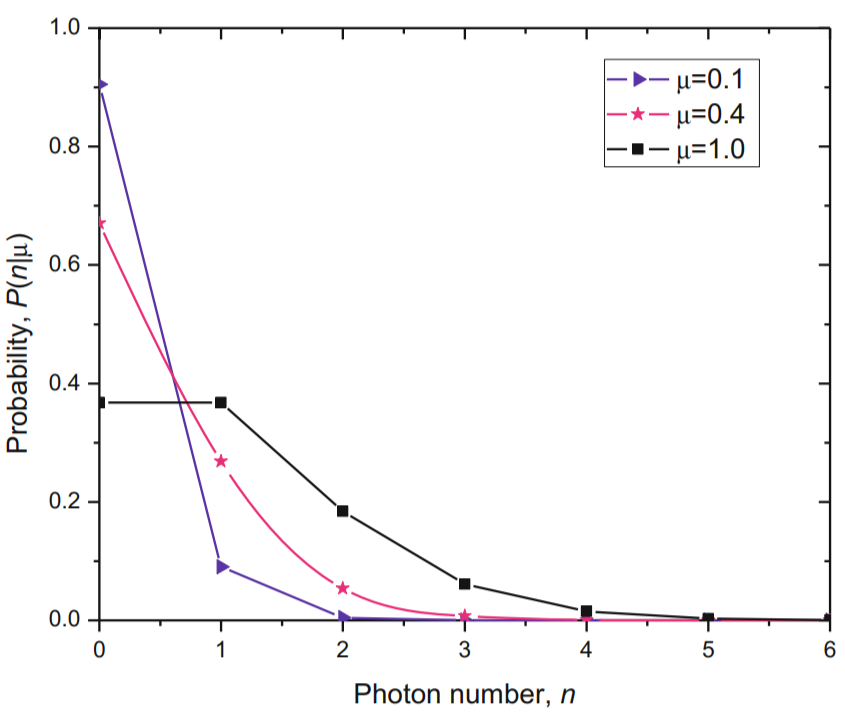
\includegraphics[width=0.7\textwidth]{chapters/figs/fig-7-11}
	\caption{توزیع تعداد فوتون (پواسون) برحسب تعداد فوتون (برای مشاهده روند، توزیع علی‌رغم گسسته بودن به‌صورت پیوسته نشان داده شده است).}
	\label{fig:7-11}
\end{figure}

با افزایش پارامتر $\mu$، احتمال دریافت بیش از یک فوتون نیز افزایش می‌یابد. برای انجام حمله \lr{PNS}، ایو می‌تواند از تقسیم‌کننده پرتو\LTRfootnote{Beam splitter (BS)} برای برداشتن یکی از فوتون‌ها از حالت چندفوتونی استفاده کند و بقیه را به باب انتقال دهد، همان‌طور که در شکل \ref{fig:7-12} تصویر شده است.


\begin{figure}[ht]
	\centering
	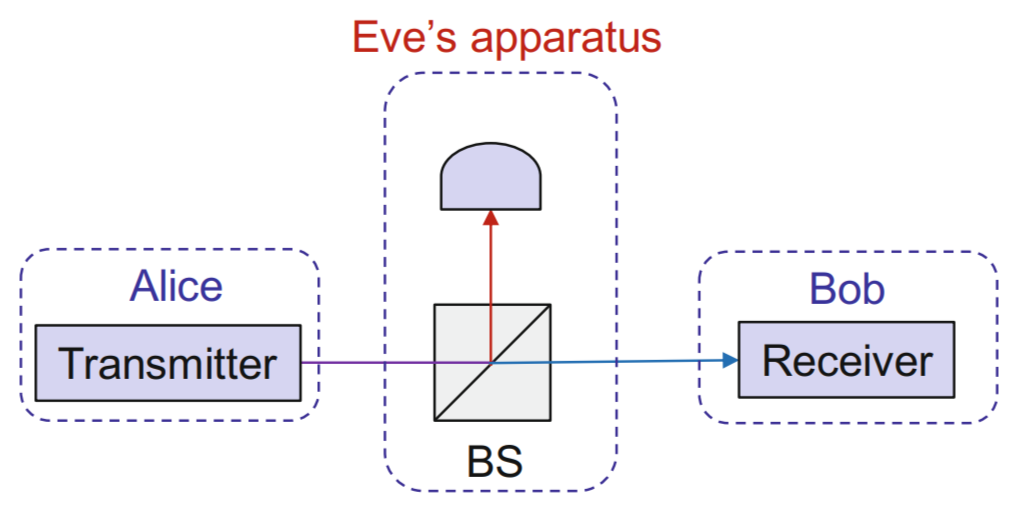
\includegraphics[width=0.6\textwidth]{chapters/figs/fig-7-12}
	\caption{تصویرسازی پیاده‌سازی حمله \lr{PNS} توسط ایو. \lr{BS}: تقسیم‌کننده پرتو.}
	\label{fig:7-12}
\end{figure}


او می‌تواند فوتون را با انتخاب تصادفی پایه اندازه‌گیری کند. ایو حتی می‌تواند پیوند کوانتومی را با فیبر با تلفات بسیار کم جایگزین کند تا آلیس و باب متوجه نشوند که سیگنال ارسالی تضعیف شده است. برای حل مشکل حمله \lr{PNS}، آلیس و باب می‌توانند از یک پروتکل مبتنی بر حالت فریب\LTRfootnote{Decoy state-based} \cite{7-35} استفاده کنند که در آن آلیس حالت‌های کوانتومی را با میانگین تعداد فوتون‌های متفاوت، که نشان‌دهنده حالت‌های سیگنال و فریب هستند، ارسال می‌کند. ایو نمی‌تواند بین حالت فریب و حالت سیگنال تمایز قائل شود و با توجه به اینکه آلیس و باب سطح سیگنال فریب را می‌دانند، می‌توانند حمله \lr{PNS} را شناسایی کنند.








\subsubsection{حملات دسته‌جمعی}
\label{subsec:7-4-1-2}
حملات دسته‌جمعی\LTRfootnote{Collective attacks} نشان‌دهنده تعمیمی از حملات غیرهمدوس هستند، با این فرض که تعامل ایو با هر کیوبیت نیز به‌صورت مستقل و با توزیع یکسان (\lr{i.i.d.}) است. با این حال، در این حملات، ایو می‌تواند کیوبیت‌های کمکی\LTRfootnote{Ancilla qubits} خود را تا پایان مراحل پس‌پردازش کلاسیک در یک حافظه کوانتومی\LTRfootnote{Quantum memory} ذخیره کند. برای مثال، با توجه به اینکه مصالحه اطلاعات مستلزم تبادل بیت‌های توازن روی یک کانال کلاسیک احرازهویت‌شده است، ایو می‌تواند بهترین حملات کلاسیک شناخته‌شده را برای یادگیری محتوای بیت‌های توازن به کار گیرد. بر اساس تمام اطلاعات در دسترس، ایو می‌تواند بهترین استراتژی اندازه‌گیری را روی کیوبیت‌های کمکی خود (ذخیره شده در حافظه کوانتومی) انجام دهد.

حمله \lr{PNS} زمانی که ایو از حافظه کوانتومی استفاده می‌کند قوی‌تر است. به‌ویژه، ایو می‌تواند از طریق فرآیند غربال‌گری متوجه شود که کدام پایه توسط آلیس استفاده شده است و می‌تواند پایه صحیح را روی فوتون ذخیره شده در حافظه کوانتومی خود اعمال کند و در نتیجه تعداد بیت‌های شناسایی شده را در مقایسه با حالتی که از حافظه کوانتومی استفاده نمی‌شود، دوبرابر کند.

کران امنیت برای حملات دسته‌جمعی، با فرض پس‌پردازش یک‌طرفه، توسط رابطه \eqref{eq:7-32} داده می‌شود که در آن اطلاعات ایو درباره دنباله آلیس از طریق اطلاعات هولِوو\LTRfootnote{Holevo information} به‌صورت زیر تعیین می‌شود \cite{7-50} (همچنین ببینید \cite{7-46}):
\begin{equation}
	I_{EA} = \max_{\text{\lr{Eve's strategies}}} \chi(\bm{A}; \bm{E}),
	\label{eq:7-36}
\end{equation}
که در آن بیشینه‌سازی روی تمام استراتژی‌های شنود دسته‌جمعی ممکن انجام می‌شود. تعریف مشابهی برای $I_{BE}$ نیز برقرار است. این کران با نام کران دوتک-وینتر\LTRfootnote{Devetak-Winter bound} نیز شناخته می‌شود. اطلاعات هولِوو که در مرجع \cite{7-51} معرفی شده است، در اینجا به‌صورت زیر تعریف می‌شود:
\begin{equation}
	\chi(\bm{A}; \bm{E}) = S(\rho_E) - \sum_a p(a) S(\rho_{E|a}),
	\label{eq:7-37}
\end{equation}
که در آن $S(\rho)$ آنتروپی فون نویمان\LTRfootnote{von Neumann entropy} است که به‌صورت $S(\rho) = -\text{Tr}(\rho \log \rho) = -\sum_i \lambda_i \log \lambda_i$ تعریف می‌شود و در آن $\lambda_i$ مقادیر ویژه عملگر (حالت) چگالی\LTRfootnote{Density operator} $\rho$ هستند. در رابطه \eqref{eq:7-37}، $p(a)$ نشان‌دهنده احتمال وقوع نماد $a$ از الفبای کلاسیک آلیس است، در حالی که $\rho_{E|a}$ عملگر چگالی متناظر با سیستم کمکی ایو است. در نهایت، $\rho_E$ حالت چگالی جزئی ایو است که به‌صورت $\rho_E = \sum_a p(a) \rho_{E|a}$ تعریف می‌شود. به عبارت دیگر، اطلاعات هولِوو متناظر با میانگین کاهش در آنتروپی فون نویمان است، با این فرض که می‌دانیم $\rho_E$ چگونه آماده‌سازی شده است.

\subsubsection{حملات همدوس}
\label{subsec:7-4-1-3}
حملات همدوس\LTRfootnote{Coherent attacks} نشان‌دهنده کلی‌ترین و منعطف‌ترین استراتژی‌هایی هستند که ایو می‌تواند روی حالت‌های کوانتومی اعمال کند. او می‌تواند استراتژی شنود را در لحظه و بر اساس اندازه‌گیری‌های قبلی و فعلی تطبیق دهد. او ممکن است حالت‌های کوانتومی متعددی را تا جایی که بخواهد درهم‌تنیده کرده و آن‌ها را در حافظه کوانتومی ذخیره کند. بنابراین، کمینه‌سازی اطلاعات متقابل بین آلیس/باب و ایو غیرممکن است. با این وجود، کران‌ها در بسیاری از موارد تعیین شده‌اند و این کران‌ها بسیار شبیه به موارد به‌دست‌آمده برای حملات دسته‌جمعی هستند. به‌ویژه، حالت‌های ارسال شده توسط آلیس $|\psi_i\rangle$ برای باب مستقل هستند و می‌توان آن‌ها را با ضرب تانسوری\LTRfootnote{Tensor product} $|\psi_1\rangle \otimes \dots \otimes |\psi_n\rangle \otimes \dots$ نشان داد و کانال کوانتومی معمولاً بین آن‌ها همبستگی ایجاد نمی‌کند.

بنابراین، ایو با معرفی همبستگی‌های مصنوعی هیچ مزیتی به‌دست نخواهد آورد. با این حال، همبستگی‌ها بعداً در طول پس‌پردازش کلاسیک معرفی می‌شوند و ایو باید به جای حدس زدن نماد ارسال شده در کلید خام، از آن همبستگی‌ها بهره‌برداری کند. کلید نهایی توسط روابط میان نمادها در کلید خام تعیین می‌شود و ایو می‌تواند با به‌کارگیری رویکردهای مبتنی بر درهم‌تنیدگی، برخی از این روابط را بیاموزد.








\subsubsection{حملات هک کوانتومی و/یا حملات کانال جانبی}
\label{subsec:7-4-1-4}
حملات هک کوانتومی\LTRfootnote{Quantum hacking attacks} از نقاط ضعف پیاده‌سازی‌های خاص سیستم‌های \lr{QKD} بهره‌برداری می‌کنند. بسیاری از این حملات با فناوری کنونی امکان‌پذیر هستند. در حمله اسب تروا\LTRfootnote{Trojan horse attack} \cite{7-52}، ایو یک باریکه لیزری درخشان را به سمت رمزگذار آلیس می‌فرستد و فوتون‌های بازتابیده را برای کسب اطلاعات درباره کلید مخفی اندازه‌گیری می‌کند. با استفاده از یک ایزولاتور نوری\LTRfootnote{Optical isolator} می‌توان از این حمله جلوگیری کرد. همچنین مشاهده شده است که شمارنده‌های فوتون مبتنی بر سیلیسیم که از فوتودیودهای بهمنی\LTRfootnote{Avalanche photodiodes (APDs)} (\lr{APD}) استفاده می‌کنند، هنگام آشکارسازی یک تک‌فوتون، مقداری نور در طول‌موج‌های مختلف ساطع می‌کنند که می‌تواند توسط ایو مورد بهره‌برداری قرار گیرد \cite{7-53}. در حمله جابه‌جایی زمانی\LTRfootnote{Time-shifting attack} \cite{7-54}، ایو از عدم تطابق بازدهی آشکارسازهای تک‌فوتون باب برای تخمین انتخاب پایه توسط او استفاده می‌کند. در حمله کورسازی\LTRfootnote{Blinding attack} \cite{7-55}، ایو از ویژگی‌های شمارنده تک‌فوتون مبتنی بر \lr{APD} بهره می‌گیرد تا باب را مجبور کند همان پایه‌ای را انتخاب کند که ایو انتخاب کرده است. \lr{APD}ها برای شمارش فوتون اغلب در مد گیت‌شده\LTRfootnote{Gated mode} عمل می‌کنند، به این معنی که \lr{APD} تنها زمانی فعال است که انتظار ورود فوتون می‌رود. وقتی \lr{APD} در وضعیت غیرفعال (خاموش) است، در یک رژیم خطی\LTRfootnote{Linear regime} عمل می‌کند، به این معنی که جریان نوری با توان نوری دریافتی متناسب است و بنابراین مانند یک فتودتکتور کلاسیک رفتار می‌کند. برای بهره‌برداری از این موضوع، ایو می‌تواند یک باریکه نور کلاسیک ضعیف ارسال کند که به اندازه کافی قوی باشد تا زمانی که باب از همان پایه ایو استفاده می‌کند «کلیک» ایجاد کند، و در غیر این صورت کلیکی ثبت نشود. در چنین سناریویی، $50\%$ از رویدادها به‌صورت بی‌نتیجه\LTRfootnote{Inconclusive} ثبت می‌شوند. خوشبختانه، ویژگی مشترک حملات هک کوانتومی این است که به محض شناخته شدن حمله، قابل پیشگیری هستند. با این حال، تهدید ناشی از حملات هک کوانتومی ناشناخته همچنان پابرجاست.

بسیاری از حملات کانال جانبی\LTRfootnote{Side-channel attacks} به‌طور هم‌زمان حملات خطای صفر\LTRfootnote{Zero-error attacks} هستند \cite{7-46}. به بیان دیگر، ایو می‌تواند از تلفات کانال کوانتومی برای پنهان کردن حمله کانال جانبی خود استفاده کند. حمله تقسیم پرتو\LTRfootnote{Beam-splitting attack} از تلفات کانال کوانتومی بهره‌برداری می‌کند؛ ایو می‌تواند یک تقسیم‌کننده پرتو را دقیقاً بعد از فرستنده آلیس قرار دهد، بخشی از باریکه را برداشته و بقیه را به باب انتقال دهد. از آنجا که آلیس مُد نوری را تغییر نمی‌دهد، این حمله توسط باب شناسایی نخواهد شد. جالب اینجاست که توزیع پواسون در طول حمله \lr{PNS} حفظ می‌شود \cite{7-56}. در پیاده‌سازی‌های واقع‌گرایانه، زمانی که آلیس از حالت‌های سیگنال مستقل خطی استفاده می‌کند، ایو می‌تواند تمایز ابهام‌ناپذیر حالت\LTRfootnote{Unambiguous state discrimination} را انجام داده و متعاقب آن سیگنال را مجدداً ارسال کند و به بازدهی بهتری نسبت به تقسیم پرتو دست یابد، همان‌طور که در مرجع \cite{7-57} نشان داده شده است. خوشبختانه، وجود حملات کانال جانبی تا زمانی که حملات مربوطه در مرحله تقویت حریم خصوصی در نظر گرفته شوند، امنیت را به خطر نمی‌اندازد \cite{7-46}.

\subsection{تعاریف امنیت}
\label{sec:7-4-2}
در اینجا ما به امنیت در برابر حملات دسته‌جمعی علاقه‌مند هستیم. فرض کنید کلید ایده‌آل نشان‌دهنده دنباله‌ای از نمادهای کاملاً همبسته بین آلیس و باب باشد که ایو هیچ اطلاعاتی از آن‌ها ندارد (کلیدهای امن مختلف از مجموعه کلیدهای امن باید به‌صورت یکنواخت ظاهر شوند). در این صورت، کلید $K$ که به اندازه $\epsilon$ از کلید ایده‌آل انحراف داشته باشد، $\epsilon$-امن\LTRfootnote{$\epsilon$-secure} نامیده می‌شود. تعاریف اولیه امنیت \lr{QKD} مشابه تعاریف کلاسیک متناظر بودند. ایو با در اختیار داشتن حالت چگالی $\rho_E$، اندازه‌گیری $\mathcal{M}$ را انجام می‌دهد که اطلاعات متقابل او با $K$ (نشان داده شده با $I(K;E)$) را بیشینه کند. این کار منجر به اطلاعات در دسترس\LTRfootnote{Accessible information} می‌شود و می‌توانیم بنویسیم:
\begin{equation}
	H(\mathcal{K} : E) = \max_{\mathcal{M}(\rho_E)=E} I(\mathcal{K} : E),
	\label{eq:7-38}
\end{equation}
که در آن بیشینه‌سازی روی تمام استراتژی‌های ممکن ایو انجام می‌شود و $H(\mathcal{K} : E)$ نشان‌دهنده اطلاعات در دسترس است. سپس $\epsilon$-امنیت را می‌توان به‌صورت زیر تعریف کرد:
\begin{equation}
	H(\mathcal{K} : E) \leq \epsilon.
	\label{eq:7-39}
\end{equation}
با توجه به اینکه ایو می‌تواند برای انجام اندازه‌گیری روی سیستم خود تا زمانی که بخشی از کلید را یاد بگیرد منتظر بماند، این نامساوی امنیت کلید را تضمین نمی‌کند.

\subsubsection{$\epsilon$-امنیت مبتنی بر فاصله اثر}
\label{subsec:7-4-2-1}
یکی از الزامات کلیدی که تعریف امنیت باید برآورده کند، ویژگی ترکیب‌پذیری\LTRfootnote{Composability} است، که نشان می‌دهد امنیت کلید صرف‌نظر از نوع کاربرد آن تضمین شده است \cite{7-46}. به عبارت دیگر، اگر کلید $\epsilon$-امن در یک وظیفه $\epsilon'$-امن استفاده شود، کل فرآیند باید حداقل $(\epsilon + \epsilon')$-امن باشد. بن-اور\LTRfootnote{Ben-Or} و همکاران در مرجع \cite{7-58} نشان داده‌اند که $\epsilon$-امنیت تعریف شده در رابطه \eqref{eq:7-39} زمانی برقرار است که در مرحله تقویت حریم خصوصی از هشینگ جهانی-$2$\LTRfootnote{Two-universal hashing} استفاده شود. از سوی دیگر، کونیگ\LTRfootnote{König} و همکاران در مرجع \cite{7-59} نشان داده‌اند که اطلاعات در دسترس برای هر $\epsilon$ دلخواه، ترکیب‌پذیر نیست.

برای مقابله با این مشکل، بن-اور و همکاران در \cite{7-58} و همچنین رنر\LTRfootnote{Renner} و کونیگ در \cite{7-60} مفهوم $\epsilon$-امنیت مبتنی بر فاصله اثر\LTRfootnote{Trace-distance-based $\epsilon$-security} را معرفی کردند (همچنین ببینید \cite{7-29, 7-43, 7-61, 7-62, 7-63}). می‌گوییم کلید نسبت به شنودگر $E$ دارای $\epsilon$-امنیت است اگر فاصله اثر بین حالت مشترک کلید $K$ و ایو $E$ (نشان داده شده با $\rho_{K,E}$) و حالت حاصل‌ضربِ حالت کاملاً مخلوط\LTRfootnote{Completely mixed state (CMS)} نسبت به مجموعه $K$ تمام کلیدهای امن ممکن (نشان داده شده با $\rho_{CMS}$) و حالت ایو (نشان داده شده با $\rho_E$)، کوچک‌تر یا مساوی $\epsilon$ باشد. به عبارت دیگر، می‌توانیم بنویسیم:
\begin{equation}
	D(\rho_{K,E}, \rho_{CMS} \otimes \rho_E) = \frac{1}{2} \|\rho_{K,E} - \rho_{CMS} \otimes \rho_E\|_1 = \frac{1}{2} \text{Tr} |\rho_{K,E} - \rho_{CMS} \otimes \rho_E| \leq \epsilon,
	\label{eq:7-40}
\end{equation}
که در آن $|\rho| = \sqrt{\rho^\dagger \rho}$ است. با این تعریف، پارامتر $\epsilon$ تفسیر کاملاً واضحی دارد: این پارامتر نشان‌دهنده حداکثر احتمال شکستِ تحمل‌پذیر برای فرآیند استخراج کلید است. با توجه به اینکه شرط ترکیب‌پذیری در این تعریف برقرار است، می‌توانیم امنیت کلید نهایی $\epsilon$ را برحسب امنیتِ مراحل تصحیح خطا (\lr{EC})\LTRfootnote{Error correction (EC)} $\epsilon_{EC}$، تقویت حریم خصوصی (\lr{PA})\LTRfootnote{Privacy amplification (PA)} $\epsilon_{PA}$ و تخمین پارامتر (\lr{PE})\LTRfootnote{Parameter estimation (PE)} $\epsilon_{PE}$؛ و همچنین احتمال شکستِ تخمین‌های آنتروپی رنی \cite{7-58} (نشان داده شده با $\epsilon_R$) تجزیه کنیم. به عبارت دیگر، می‌توانیم بنویسیم $\epsilon = \epsilon_{EC} + \epsilon_{PA} + \epsilon_{PE} + \epsilon_R$.

اکنون پرسش اصلی این است که چگونه تعریف $\epsilon$-امنیت مبتنی بر فاصله اثر را به طول $m$ کلید مخفی استخراج‌شده مرتبط کنیم. برای این کار، نیاز است نامساوی زیر که نشان‌دهنده تعمیم کران چرنوف\LTRfootnote{Chernoff bound} است، اثبات شود \cite{7-46}:
\begin{equation}
	\text{Pr} \left( D(\rho_{K,E}, \rho_{CMS} \otimes \rho_E) > \epsilon \right) \leq e^{m - f(\rho_{K,E}, \epsilon)},
	\label{eq:7-41}
\end{equation}
که در آن ضرایب ثابت حذف شده‌اند. به‌وضوح، کلید با احتمال بسیار کمی ناامن خواهد بود، به شرطی که شرط زیر برقرار باشد:
\begin{equation}
	m \leq f(\rho_{K,E}, \epsilon).
	\label{eq:7-42}
\end{equation}
به عبارت دیگر، تا زمانی که طول کلید کوتاه‌تر از عدم قطعیت ایو درباره ورودیِ مرحله تقویت حریم خصوصی باشد، کلید امن خواهد بود. کران‌های امنیت بحث شده در بخش \ref{sec:7-4-1} به‌صورت مجانبی برای کلیدهای بی‌نهایت طولانی، زمانی که $\epsilon \to 0$ است، معتبر هستند.








\subsubsection{$\epsilon$-امنیت مبتنی بر وفاداری}
\label{subsec:7-4-2-2}
علاوه بر $\epsilon$-امنیت مبتنی بر فاصله اثر، می‌توان از مفهوم $\epsilon$-امنیت مبتنی بر وفاداری\LTRfootnote{Fidelity-based $\epsilon$-security} نیز استفاده کرد \cite{7-58}. فرض کنیم آلیس دارای $n$ جفت کیوبیت درهم‌تنیده $|B_{00}\rangle = (|00\rangle + |11\rangle)/\sqrt{2}$ باشد که به‌صورت $|B_{00}\rangle^{\otimes n}$ نشان داده می‌شود. وفاداری\LTRfootnote{Fidelity} دو حالت چگالی $\rho$ و $\rho'$ به‌صورت زیر تعریف می‌شود:
\begin{equation}
	F(\rho, \rho') = \text{Tr} \left( \sqrt{\rho^{1/2} \rho' \rho^{1/2}} \right).
	\label{eq:7-43}
\end{equation}
زمانی که $\rho = |\psi\rangle\langle\psi|$ و $\rho' = |\psi'\rangle\langle\psi'|$ حالت‌های خالص باشند، با توجه به اینکه برای حالت‌های خالص $\rho^2 = \rho$ است، وفاداری به‌سادگی به‌صورت زیر در می‌آید:
\begin{equation}
	F(\rho, \rho') = \text{Tr} \sqrt{|\psi\rangle\langle\psi|\psi'\rangle\langle\psi'|\psi\rangle\langle\psi|} = |\langle \psi | \psi' \rangle|.
	\label{eq:7-44}
\end{equation}
وفاداری بین حالت خالص $|\psi\rangle$ و حالت چگالی دلخواه $\rho$ به‌صورت زیر داده می‌شود:
\begin{equation}
	F(\rho, |\psi\rangle) = \text{Tr} \sqrt{|\psi\rangle\langle\psi| \rho |\psi\rangle\langle\psi|} = \text{Tr} \sqrt{\langle\psi|\rho|\psi\rangle |\psi\rangle\langle\psi|} = \sqrt{\langle \psi | \rho | \psi \rangle}.
	\label{eq:7-45}
\end{equation}
یک قضیه مهم مرتبط با وفاداری، قضیه اولمان\LTRfootnote{Uhlmann theorem} است \cite{7-64}، که بیان می‌کند برای دو عملگر چگالی $\rho$ و $\rho'$ و در صورتی که پالایش\LTRfootnote{Purification} حالت $\rho$ به‌صورت $|\psi\rangle\langle\psi|$ باشد، رابطه زیر برقرار است:
\begin{equation}
	F(\rho, \rho') = \max_{|\psi'\rangle\langle\psi'|} F(|\psi\rangle\langle\psi|, |\psi'\rangle\langle\psi'|),
	\label{eq:7-46}
\end{equation}
که در آن بیشینه‌سازی روی تمام پالایش‌های $|\psi'\rangle\langle\psi'|$ از $\rho'$ انجام می‌شود. با اعمال رابطه \eqref{eq:7-45} روی $|B_{00}\rangle^{\otimes n}$، به‌دست می‌آوریم:
\begin{equation}
	F^2(\rho_{AB}^n, |B_{00}\rangle^{\otimes n}) = \prescript{\otimes n}{}{\langle} B_{00} | \rho_{AB}^n | B_{00} \rangle^{\otimes n},
	\label{eq:7-47}
\end{equation}
که در آن $\rho_{AB}^n$ حالت چگالی مشترک بین آلیس و باب است. کلیدهای نهایی برای آلیس و باب که به‌ترتیب با $\mathcal{K}_A$ و $\mathcal{K}_B$ نشان داده می‌شوند، دارای طول $m < n$ هستند و در غیاب ایو، $\rho_{AB}^m$ برابر با $|B_{00}\rangle^{\otimes m}$ خواهد بود. بنابراین، می‌توانیم $\epsilon$-امنیت مبتنی بر وفاداری را به‌صورت زیر تعریف کنیم:
\begin{equation}
	1 - F(\rho_{AB}^m, |B_{00}\rangle^{\otimes m}) \leq \epsilon''.
	\label{eq:7-48}
\end{equation}
بنابراین در غیاب ایو، $F(\rho_{AB}^m, |B_{00}\rangle^{\otimes m}) = 1$ است و به‌وضوح در آن حالت $0 = \epsilon''$ خواهد بود. فرض کنید $|\psi_1^m\rangle\langle\psi_1^m|$ پالایش $\rho_{ABE}^m$ روی سیستم‌های $A$، $B$ و $E$ باشد. طبق قضیه اولمان، پالایشی مانند $|\psi_1^m\rangle\langle\psi_1^m|$ وجود دارد به‌طوری که:
\begin{equation}
	F(|\psi_1^m\rangle\langle\psi_1^m|, |\psi_2^m\rangle\langle\psi_2^m|) = F(\rho_{AB}^m, |B_{00}\rangle^{\otimes m}).
	\label{eq:7-49}
\end{equation}
با ساخت مناسب حالت‌های پالایش $|\psi_1^m\rangle$ و $|\psi_2^m\rangle$ و انجام اندازه‌گیری‌ها روی سیستم آلیس و باب، در حالی که اثر جزئی روی سیستم ایو گرفته می‌شود، به‌دست می‌آوریم:
\begin{equation}
	F(\rho_{\text{QKD}}^m, \rho_{\text{perfect}}^m) > F(\rho_{AB}^m, |B_{00}\rangle^{\otimes m}),
	\label{eq:7-50}
\end{equation}
که در آن $\rho_{\text{perfect}}^m$ عملگر چگالی متناظر با کلید ایده‌آل\LTRfootnote{Perfect key} است؛ کلیدی که توزیع آن روی دو رشته به طول $m$ به‌صورت $p_{\text{perfect}}^{(m)}(l, l') = \delta(l, l') 2^{-m}$ است \cite{7-58}. در رابطه \eqref{eq:7-50}، $\rho_{\text{QKD}}^m$ نشان‌دهنده عملگر چگالی متناظر با طرح \lr{QKD} است. به عبارت دیگر، با انجام پالایش دو حالت چگالی، وفاداری بهبود می‌یابد. با توجه به اینکه فاصله اثر و وفاداری طبق مراجع \cite{7-6, 7-61} با هم مرتبط هستند:
\begin{equation}
	\|\rho_{\text{QKD}}^m - \rho_{\text{perfect}}^m\|_1 \leq 2 \sqrt{1 - F(\rho_{\text{QKD}}^m, \rho_{\text{perfect}}^m)},
	\label{eq:7-51}
\end{equation}
نتیجه می‌گیریم که $\epsilon$-امنیت مبتنی بر وفاداری با $\epsilon$-امنیت مبتنی بر فاصله اثر مرتبط است، زیرا:
\begin{equation}
	\frac{1}{2} \|\rho_{\text{QKD}}^m - \rho_{\text{perfect}}^m\|_1 \leq \sqrt{\epsilon''},
	\label{eq:7-52}
\end{equation}
و بنابراین تعریف $\epsilon$-امنیت مبتنی بر وفاداری نیز ترکیب‌پذیر\LTRfootnote{Composable} است.

اگر وفاداری بالا باشد، آنگاه عدد صحیح مثبت $s$ وجود دارد به‌طوری که:
\begin{equation*}
	F^2(\rho_{AB}^m, |B_{00}\rangle^{\otimes m}) = \prescript{\otimes m}{}{\langle} B_{00} | \rho_{AB}^m | B_{00} \rangle^{\otimes m} > 1 - 2^{-s}.
\end{equation*}
به‌وضوح، بزرگ‌ترین مقدار ویژه $\rho_{AB}^m$ باید بزرگ‌تر از $1 - 2^{-s}$ باشد. آنتروپی فون نویمان\LTRfootnote{von Neumann entropy} برای $\rho_{AB}^m$ از بالا توسط آنتروپی عملگر چگالی زیر محدود می‌شود \cite{7-6}:
\begin{equation}
	\bm{\rho}_{\max} = \text{diag} \left( 1 - 2^{-s}, \underbrace{\frac{2^{-s}}{2^{2m}-1}, \dots, \frac{2^{-s}}{2^{2m}-1}}_{2^{2m}-1 \text{ entries}} \right)
	\label{eq:7-53}
\end{equation}
که به‌صورت زیر داده می‌شود:
\begin{equation}
	S_{\max} = S(\bm{\rho}_{\max}) = -(1 - 2^{-s}) \log(1 - 2^{-s}) - (2^{2n} - 1) \frac{2^{-s}}{2^{2m}-1} \log \left( \frac{2^{-s}}{2^{2m}-1} \right).
	\label{eq:7-54}
\end{equation}
با استفاده از تقریب $x \approx \ln(1+x)$ زمانی که $x$ کوچک باشد، به‌دست می‌آوریم:
\begin{equation}
	S_{\max} \leq (1 - 2^{-s}) 2^{-s} / \ln 2 + 2^{-s}s + 2^{-s}2m = (2m + s + 1/\ln 2) 2^{-s} - \underbrace{\frac{2^{-2s}}{\ln 2}}_{O(2^{-2s})}.
	\label{eq:7-55}
\end{equation}
در نتیجه، وفاداری بالا به معنای آنتروپی فون نویمان پایین است زیرا:
\begin{equation}
	S(\rho_{AB}^m) < S_{\max} \leq (2m + s + 1/\ln 2) 2^{-s} - O(2^{-2s}).
	\label{eq:7-56}
\end{equation}
بنابراین، با حصول اطمینان از اینکه آلیس و باب جفت‌های \lr{EPR} با وفاداری حداقل $1 - 2^{-s}$ در اختیار دارند، پروتکل \lr{QKD} امن خواهد بود \cite{7-6}.




\subsubsection{نرخ‌های کلید امن برای سیستم‌های \lr{DV-QKD} دوبعدی}
\label{subsec:7-4-3}
کران مربوط به طرح‌های \lr{DV-QKD} دوبعدی (\lr{2-D})، با فرض حملات انفرادی، توسط روابط \eqref{eq:7-32} و \eqref{eq:7-33} داده می‌شود. اطلاعات متقابل بین آلیس و باب را می‌توان با به‌کارگیری کانال متقارن باینری\LTRfootnote{Binary symmetric channel (BSC)} (\lr{BSC}) تعیین کرد، که در آن برای احتمال خطای $q$، که در \lr{DV-QKD} معمولاً نرخ خطای بیت کوانتومی\LTRfootnote{Quantum bit-error rate (QBER)} (\lr{QBER}) نامیده می‌شود، اطلاعات متقابل به‌صورت $I(A; B) = 1 - h(q)$ تعیین می‌گردد. برای در نظر گرفتن گام ناقص مصالحه اطلاعات، یا به‌طور معادل کدگذاری کنترل خطا\LTRfootnote{Error control coding (ECC)} (\lr{ECC})، نشت اطلاعات \lr{ECC} به ایو که با $\text{leakage}_{\text{ECC}}(q)$ نشان داده می‌شود \cite{7-46}، به‌وضوح از پایین توسط $h(q)$ محدود می‌گردد؛ بنابراین می‌توانیم عبارت \lr{SKR} را به‌صورت زیر بازنویسی کنیم:
\begin{equation}
	\text{SKR} = R_{\text{raw}} [1 - \text{leakage}_{\text{ECC}}(q) - I_E], \quad I_E = \min_{\text{Eve's strategies}} (I_{EA}, I_{EB}).
	\label{eq:7-57}
\end{equation}
عبارتی مشابه این در مراجع \cite{7-65, 7-66, 7-67, 7-68} استخراج شده است. ما فرض می‌کنیم که ایو تنها می‌تواند برای بازه‌های زمانی غیرخالی اطلاعات کسب کند، به شرطی که باب آنچه را که ایو برای او مجدداً ارسال کرده است، آشکارسازی کند. با توجه به اینکه منبع آلیس را می‌توان به‌صورت ارسال پالسی حاوی $n$ فوتون با احتمال $p_{A,n}$ بازنمایی کرد، می‌توانیم قضیه دِ فینتی\LTRfootnote{de Finetti theorem} \cite{7-61} را اعمال کنیم؛ در این صورت می‌توانیم اطلاعات ایو $I_E$ را برحسب $I_E$ برای هر تعداد فوتون به‌صورت زیر تجزیه کنیم:
\begin{equation}
	I_E = \min(I_{EA}, I_{EB}) = \min_{\text{Eve's strategies}} \left\{ \max \left( \sum_n I_{EA,n} y_n \right), \max \left( \sum_n I_{EB,n} y_n \right) \right\},
	\label{eq:7-58}
\end{equation}
که در آن $y_n = R_{\text{raw},n}/R_{\text{raw}}$ است و نشان‌دهنده کسرِ نرخ کلید خام کل در زمانی است که آلیس از $n$ فوتون در هر پالس استفاده کرده است.





\subsubsection{پروتکل BB84 آماده‌سازی-و-اندازه‌گیری}
\label{subsec:7-4-3-1}
در پروتکل \lr{BB84} آماده‌سازی-و-اندازه‌گیری\LTRfootnote{Prepare-and-measure}، $I_{EA} = I_{EB}$ است و عبارت \eqref{eq:7-58} به صورت $I_E = \max (\sum_{n} I_{EA,n} y_n)$ ساده می‌شود. در حالت صفر-فوتونی، واضح است که $I_{EA,0} = 0$ است. برای حالت تک-فوتونی، تنها راهی که ایو می‌تواند مقداری اطلاعات کسب کند، به‌کارگیری حمله سد کردن-بازارسال\LTRfootnote{Intercept-resend (IR)} است که نرخ خطای $q_1$ را معرفی می‌کند و اطلاعات متناظر ایو $I_{EA,1} = h(q_1)$ خواهد بود. برای تعداد فوتون‌های دو و بیشتر در هر پالس، ایو از حمله \lr{PNS} استفاده می‌کند و اطلاعات او در این حالت برابر با $1$ است، یعنی $I_{EA,n} = 1$ برای $n \geq 2$. به‌وضوح، بر اساس این بحث، نتیجه می‌گیریم که اطلاعات ایو به‌صورت زیر خواهد بود:
\begin{equation}
	\begin{aligned}
		I_E &= \max_{\text{Eve's strategies}} \sum_{n} I_{EA,n} y_n = \max_{\text{Eve's strategies}} [y_1 h(q_1) + y_{n \geq 2}] \\
		&= \max_{\text{Eve's strategies}} [y_1 h(q_1) + 1 - y_0 - y_1] = 1 - \min_{\text{Eve's strategies}} \{ y_0 + y_1 [1 - h(q_1)] \}.
	\end{aligned}
	\label{eq:7-59}
\end{equation}
در طرح‌های \lr{QKD} دوبعدی آماده‌سازی-و-اندازه‌گیری، مانند \lr{BB84}، تنها پارامترهایی که اندازه‌گیری می‌شوند نرخ کلید خام $R_{\text{raw}} = \sum_n R_{\text{raw},n}$ و میانگین نرخ خطای بیت کوانتومی (\lr{QBER}) $q = \sum_n q_n y_n$ هستند. در این صورت، باید فرض کنیم که برای $n \geq 2$ مقدار $q_n = 0$ است، به‌طوری که $q_1 = q/y_1$ شود. علاوه‌بر این، در رابطه \eqref{eq:7-31} منطقی است که $p_0 = 0$ و برای $n \geq 2$ مقدار $p_n = 0$ قرار داده شود تا بتوانیم بنویسیم:
\begin{equation}
	R_{\text{raw}} = R_{\text{raw},1} + R_{\text{raw},n \geq 2} = R_{\text{raw},1} + R_s p_{\text{sift}} p_{A,n \geq 2},
	\label{eq:7-60}
\end{equation}
و پس از تقسیم هر دو طرف معادله بر $R_{\text{raw}}$، راه حل زیر را برای $y_1 = R_{\text{raw},1}/R_{\text{raw}}$ به‌دست می‌آوریم \cite{7-68}:
\begin{equation}
	y_1 = 1 - (R_s/R_{\text{raw}}) p_{\text{sift}} p_{A,n \geq 2}.
	\label{eq:7-61}
\end{equation}
برای این $y_1$، رابطه \eqref{eq:7-59} به‌صورت زیر در می‌آید:
\begin{equation}
	I_E = 1 - y_1 [1 - h(q_1)] = 1 - y_1 [1 - h(q/y_1)].
	\label{eq:7-62}
\end{equation}
در نهایت، پس از جایگذاری $I_E$ استخراج‌شده در رابطه \eqref{eq:7-57}، معادله زیر را برای \lr{SKR} به‌دست می‌آوریم:
\begin{equation}
	\text{SKR} = R_{\text{raw}} [y_1 (1 - h(q/y_1)) - \text{leakage}_{\text{ECC}}(q)].
	\label{eq:7-63}
\end{equation}

\subsubsection{پروتکل مبتنی بر حالت فریب}
\label{subsec:7-4-3-2}
در ادامه این بخش، \lr{QKD} دوبعدی را با استفاده از حالت‌های فریب\LTRfootnote{Decoy states} مطالعه می‌کنیم \cite{7-35, 7-69, 7-70, 7-71, 7-72, 7-73, 7-74, 7-75, 7-76}. در پروتکل‌های مبتنی بر حالت فریب، آلیس ماهیت سیگنال کوانتومی (مانند شدت لیزر) را به‌طور تصادفی تغییر می‌دهد. در پایان فرآیند ارسال، او فاش می‌کند که از چه شدت‌هایی استفاده کرده است تا ایو نتواند حمله خود را در حین اجرا تطبیق دهد. در مرحله پس‌پردازش، آلیس و باب از این اطلاعات برای تخمین پارامتر استفاده می‌کنند. آلیس و باب می‌توانند کسر مخفی را با بهینه‌سازی هم روی سطوح سیگنال و هم روی احتمال وقوع هر سطح، بیشینه کنند. در عمل، حتی در حضور اثرات تلاطم اتمسفری، همان‌طور که در \cite{7-77} نشان داده شده است، سه سطح کافی می‌باشد. فرض کنید $p$ برخی پارامترهای منبع باشد که قابل تنظیم هستند، مانند میانگین تعداد فوتون $\mu$ (یا شدت) منبع لیزر. آلیس مقدار پارامتر $p$ را به‌طور تصادفی از پالس به پالس تغییر می‌دهد و در پایان فاز ارسال کلید خام، فهرست مقادیر $p \in \mathcal{P}$ را فاش می‌کند. آلیس و باب داده‌های موجود را دسته‌بندی کرده و تخمین پارامتر را انجام می‌دهند. آلیس و باب $2|\mathcal{P}|$ پارامتر $R_{\text{raw}}^{(p)}$ و $q^{(p)}$ را برای $p = 1, \dots, |\mathcal{P}|$ اندازه‌گیری می‌کنند. مجموعه پارامترهای $\mathcal{P}$ به‌صورت عمومی شناخته می‌شود؛ با این حال، برای $|\mathcal{P}| > 1$ ایو نمی‌تواند استراتژی اندازه‌گیری خود را بر اساس $p$ تطبیق دهد، زیرا از قبل آن را نمی‌داند. بدیهی است که $p_n$ و $q_n$ مستقل از $p$ هستند. نرخ کلید خام زمانی که آلیس پالسی با $n$ فوتون ارسال می‌کند به‌صورت $R_{\text{raw},n}^{(p)} = R_s p_{\text{sift}} p_{A,n}^{(p)} p_n$ می‌شود. پارامترهای اندازه‌گیری شده به‌صورت زیر در می‌آیند:
\begin{equation}
	R_{\text{raw}}^{(p)} = \sum_{n \geq 0} R_{\text{raw},n}^{(p)}, \quad q^{(p)} = \sum_{n \geq 0} q_n^{(p)} y_n^{(p)}; \quad p = 1, 2, \dots, |\mathcal{P}|
	\label{eq:7-64}
\end{equation}
معادله فوق یک سیستم خطی از $2|\mathcal{P}|$ معادله برای $p_n$ و $q_n$ معرفی می‌کند. همان‌طور که در بالا ذکر شد، در عمل پروتکل حالت فریب با $|\mathcal{P}| = 3$ عملکردی قابل مقایسه با حالت ایده‌آل دارد \cite{7-76, 7-77}. برای هر $p$، اطلاعات ایو به‌صورت زیر داده می‌شود:
\begin{equation}
	I_E^{(p)} = 1 - y_0^{(p)} - y_1^{(p)} [1 - h(q_1)]; \quad y_n^{(p)} = R_{\text{raw},n}^{(p)}/R_{\text{raw}}^{(p)}, \quad n = 0, 1
	\label{eq:7-65}
\end{equation}
\lr{SKR} کل را می‌توان با جمع کردن \lr{SKR}ها برای مقادیر مختلف $p$ به‌دست آورد، یعنی $\text{SKR} = \sum_p \text{SKR}^{(p)}$. هنگامی که پس‌پردازش کلاسیک روی کل کلید خام اعمال شده باشد، \lr{SKR} به‌صورت زیر ساده می‌شود:
\begin{equation}
	\text{SKR} = R_{\text{raw}} [1 - \text{leakage}_{\text{ECC}}(q)] - \sum_p R_{\text{raw}}^{(p)} I_E^{(p)}.
	\label{eq:7-66}
\end{equation}






\section{مبانی اپتیک کوانتومی}
\label{sec:7-5}
در این بخش، برای تسهیل در تشریح طرح‌های \lr{CV-QKD}، به‌اختصار مبانی اپتیک کوانتومی \cite{7-7, 7-30, 7-78, 7-79, 7-80} را شرح می‌دهیم. برای مطالعه توصیف تفصیلی اپتیک کوانتومی، خواننده علاقه‌مند به فصل \ref{chap:6} ارجاع داده می‌شود. یک موج تخت تک‌فام\LTRfootnote{Monochromatic plane wave} را می‌توان به‌صورت زیر نمایش داد:
\begin{equation}
	\bm{E}(\bm{r}, t) = \bm{e} |\bm{E}| [I \cos(\bm{k}\bm{r} - \omega t) - Q \sin(\bm{k}\bm{r} - \omega t)]
	\label{eq:7-67}
\end{equation}
که در آن مؤلفه اول نشان‌دهنده هم‌فاز\LTRfootnote{In-phase} و مؤلفه دوم نشان‌دهنده مؤلفه مربعی\LTRfootnote{Quadrature component} است. بردار $\bm{e}$ جهت‌گیری قطبش را نشان می‌دهد، $\bm{k}$ بردار موج و $\bm{r}$ بردار مکان است.

\subsection{عملگرهای مربعی، عملگرهای تولید و نابودی، اصل عدم قطعیت}
\label{subsec:7-5-1}
در اپتیک کوانتومی، مؤلفه‌های مربعی $I$ و $Q$ با عملگرهای متناظر $\hat{I}$ و $\hat{Q}$ جایگزین می‌شوند که معادل عملگرهای مکان و تکانه هستند و در رابطه جابه‌جایی مشابهی صدق می‌کنند:
\begin{equation}
	[\hat{I}, \hat{Q}] = 2jN_0,
	\label{eq:7-68}
\end{equation}
که در آن $N_0$ نشان‌دهنده واریانس نوسان خلأ (نویز شات\LTRfootnote{Shot noise}) است. (اغلب در اپتیک کوانتومی، نمادگذاری متفاوتی برای عملگرهای مربعی استفاده می‌شود؛ به‌ویژه به جای آن‌ها از $\hat{x}$ و $\hat{p}$ استفاده می‌گردد.) حالت‌های ویژه $\hat{I}$ را می‌توان با $|I\rangle$ نشان داد، زیرا $\hat{I}|I\rangle = I|I\rangle$ است.
عملگرهای نابودی\LTRfootnote{Annihilation operator} $a$ و تولید\LTRfootnote{Creation operator} $a^\dagger$ به‌صورت زیر تعریف می‌شوند:
\begin{equation}
	a = \frac{\hat{I} + j\hat{Q}}{2\sqrt{N_0}}, \quad a^\dagger = \frac{\hat{I} - j\hat{Q}}{2\sqrt{N_0}}.
	\label{eq:7-69}
\end{equation}
به عبارت دیگر، می‌توانیم عملگرهای مربعی را برحسب عملگرهای نابودی و تولید به‌صورت زیر بیان کنیم:
\begin{equation}
	\hat{I} = (a^\dagger + a)\sqrt{N_0}, \quad \hat{Q} = j(a^\dagger - a)\sqrt{N_0}.
	\label{eq:7-70}
\end{equation}
عملگر تعداد فوتون پیش‌تر به‌صورت زیر معرفی شده بود:
\begin{equation}
	\hat{N} = a^\dagger a = \frac{\hat{I} + j\hat{Q}}{2\sqrt{N_0}} \frac{\hat{I} - j\hat{Q}}{2\sqrt{N_0}} = \frac{1}{4N_0} \left[ (\hat{I}^2 + \hat{Q}^2) - j \underbrace{(\hat{I}\hat{Q} - \hat{Q}\hat{I})}_{[\hat{I}, \hat{Q}] = 2N_0 j} \right] = \frac{1}{4N_0} [(\hat{I}^2 + \hat{Q}^2) + 2N_0],
	\label{eq:7-71}
\end{equation}
حالت‌های فوک\LTRfootnote{Fock states} (حالت‌های تعداد فوتون) کِت‌های ویژه عملگر تعداد فوتون هستند:
\begin{equation}
	\hat{N}|n\rangle = n|n\rangle,
	\label{eq:7-72}
\end{equation}
که در آن $n$ نشان‌دهنده تعداد فوتون‌ها است.
حالت خلأ\LTRfootnote{Vacuum state} که با $|0\rangle$ نشان داده می‌شود، یک کِت ویژه از عملگر نابودی است:
\begin{equation}
	a|0\rangle = 0 \Rightarrow \langle 0 | a^\dagger a | 0 \rangle = 0.
	\label{eq:7-73}
\end{equation}
حالت همدوس $| \alpha \rangle$ که پیش‌تر معرفی شد، کِت ویژه راستِ عملگر نابودی $a$ است؛ یعنی $a|\alpha\rangle = \alpha|\alpha\rangle$ که در آن $\alpha$ مقدار ویژه مختلط است. مقادیر چشم‌داشتی\LTRfootnote{Expected values} عملگرهای مربعی نسبت به حالت $|\alpha\rangle$ به‌صورت زیر داده می‌شوند:
\begin{equation}
	\begin{aligned}
		\langle \hat{I} \rangle_\alpha &= \langle \alpha | \hat{I} | \alpha \rangle = \langle \alpha | (a + a^\dagger) | \alpha \rangle \sqrt{N_0} = \langle \alpha | (\alpha + \alpha^*) | \alpha \rangle \sqrt{N_0} = 2\text{Re}\{\alpha\}\sqrt{N_0}, \\
		\langle \hat{Q} \rangle_\alpha &= \langle \alpha | \hat{Q} | \alpha \rangle = j\langle \alpha | (a^\dagger - a) | \alpha \rangle \sqrt{N_0} = j\langle \alpha | (\alpha^* - \alpha) | \alpha \rangle \sqrt{N_0} = 2\text{Im}\{\alpha\}\sqrt{N_0}.
	\end{aligned}
	\label{eq:7-74}
\end{equation}
بنابراین، اگر ضریب مقیاس $1/(2\sqrt{N_0})$ را بر $\alpha$ اعمال کنیم، مقادیر چشم‌داشتی عملگرهای هم‌فاز و مربعی نشان‌دهنده بخش‌های حقیقی و موهومی $\alpha$ خواهند بود. برای حالت خلأ، مقادیر چشم‌داشتی عملگرهای مربعی برابر با صفر است و بنابراین، رابطه \eqref{eq:7-74} جابه‌جایی\LTRfootnote{Displacement} را تعریف می‌کند. مقادیر چشم‌داشتی $\hat{I}^2$ و $\hat{Q}^2$ به‌صورت زیر داده می‌شوند:
\begin{equation}
	\begin{aligned}
		\langle \hat{I}^2 \rangle_\alpha &= \langle \alpha | \hat{I}^2 | \alpha \rangle = \langle \alpha | (a + a^\dagger)(a + a^\dagger) | \alpha \rangle N_0 = [(\alpha + \alpha^*)^2 + 1] N_0, \\
		\langle \hat{Q}^2 \rangle_\alpha &= \langle \alpha | \hat{Q}^2 | \alpha \rangle = j^2 \langle \alpha | (a^\dagger - a)(a^\dagger - a) | \alpha \rangle N_0 = [1 - (\alpha^* - \alpha)^2] N_0.
	\end{aligned}
	\label{eq:7-75}
\end{equation}
واریانس‌های متناظر برای عملگرهای مربعی در این صورت برابر خواهند بود با:
\begin{equation}
	\begin{aligned}
		\langle \Delta \hat{I}^2 \rangle_\alpha &= \langle \hat{I}^2 \rangle_\alpha - \langle \hat{I} \rangle_\alpha^2 = [(\alpha + \alpha^*)^2 + 1] N_0 - (\alpha + \alpha^*)^2 N_0 = N_0, \\
		\langle \Delta \hat{Q}^2 \rangle_\alpha &= \langle \hat{Q}^2 \rangle_\alpha - \langle \hat{Q} \rangle_\alpha^2 = [1 - (\alpha^* - \alpha)^2] N_0 + (\alpha^* - \alpha)^2 N_0 = N_0,
	\end{aligned}
	\label{eq:7-76}
\end{equation}
که نشان می‌دهد واریانس‌های نوسانات برای هر دو مؤلفه مربعی یکسان است. با قرار دادن $\alpha = 0$، همین نتیجه برای حالت خلأ نیز صدق می‌کند. حاصل‌ضرب واریانس‌های مؤلفه‌های مربعی به‌صورت زیر داده می‌شود:
\begin{equation}
	\langle \Delta \hat{I}^2 \rangle_\alpha \langle \Delta \hat{Q}^2 \rangle_\alpha = N_0^2,
	\label{eq:7-77}
\end{equation}
که نشان می‌دهد اصل عدم قطعیت هایزنبرگ با علامت تساوی برقرار است. به عبارت دیگر، حالت همدوس در رابطه کمینه عدم قطعیت صدق می‌کند. اصل عدم قطعیت در سیستم‌های \lr{CV-QKD} به‌کار گرفته می‌شود. اغلب اصل عدم قطعیت برحسب واحد نویز شات\LTRfootnote{Shot noise unit (SNU)} بیان می‌شود، جایی که $N_0$ به $1$ نرمالیزه شده است، به‌صورت زیر: $\Delta \hat{I}^2 \Delta \hat{Q}^2 \geq 1$.






\subsection{حالت‌های همدوس، حالت گاوسی و حالت‌های فشرده}
\label{subsec:7-5-2}
حالت گاوسی\LTRfootnote{Gaussian state} یک حالت همدوس است که در آن تصویرها در امتداد کِت‌های ویژه $\hat{I}$ دارای شکل گاوسی هستند:
\begin{equation}
	\langle I|\alpha \rangle = \frac{1}{(2\pi N_0)^{1/4}} \exp\left[ -\frac{(I-\langle I \rangle)^2 + j\langle I \rangle \langle Q \rangle}{4N_0} + \frac{j I \langle Q \rangle}{2N_0} \right].
	\label{eq:7-78}
\end{equation}
حالت فشرده\LTRfootnote{Squeezed state} یک حالت گاوسی خاص است که دارای نوسانات نابرابر در مؤلفه‌های مربعی\LTRfootnote{Quadratures} است:
\begin{equation}
	\begin{aligned}
		\langle I|\alpha, s \rangle = \frac{1}{(2\pi N_0 s)^{1/4}} \exp\left[ -\frac{s^{-1}(I-\langle I \rangle)^2 + j\langle I \rangle \langle Q \rangle}{4N_0} + \frac{j I \langle Q \rangle}{2N_0} \right], \quad s > 0 \\
		V(\hat{I}) = \text{Var}(\hat{I}) = sN_0, \quad V(\hat{Q}) = \text{Var}(\hat{Q}) = s^{-1} N_0,
	\end{aligned}
	\label{eq:7-79}
\end{equation}
که در آن $s$ پارامتر فشردگی\LTRfootnote{Squeezing parameter} است.
برای تجسم حالت‌های کوانتومی در اپتیک کوانتومی، از تابع ویگنر\LTRfootnote{Wigner function} استفاده می‌شود که برای حالت چگالی\LTRfootnote{Density state} $\rho$ به‌صورت زیر تعریف می‌گردد \cite{7-7}:
\begin{equation}
	W(I, Q) = \frac{1}{4\pi N_0} \int e^{\frac{j \xi Q}{2N_0}} \langle I - \xi/2 | \rho | I + \xi/2 \rangle d\xi.
	\label{eq:7-80}
\end{equation}
اگر کسی مؤلفه هم‌فاز را اندازه‌گیری کند، نتیجه از تابع چگالی احتمال\LTRfootnote{Probability density function (PDF)} (\lr{PDF}) $f(I)$ پیروی می‌کند که با میانگین‌گیری از تابع ویگنر روی مؤلفه مربعی به‌دست می‌آید، یعنی $f(I) = \int W(I, Q) dQ$. از سوی دیگر، اگر کسی مؤلفه مربعی را اندازه‌گیری کند، نتیجه از \lr{PDF} مقابل پیروی خواهد کرد: $f(Q) = \int W(I, Q) dI$. بنابراین، می‌توانیم تابع ویگنرِ حالت همدوس $|\alpha\rangle$ را به‌عنوان یک توزیع گاوسی دو‌بعدی به مرکزیت $(\text{Re}\{\alpha\}, \text{Im}\{\alpha\})$ با واریانس $N_0$ (و کوواریانس صفر) تفسیر کنیم. در نتیجه، در صفحه $(I, Q)$ حالت همدوس توسط یک دایره نمایش داده می‌شود که شعاع آن با انحراف معیار (عدم قطعیت) مرتبط است، همان‌طور که در شکل \ref{fig:7-13} تصویر شده است.






\begin{figure}[ht]
	\centering
	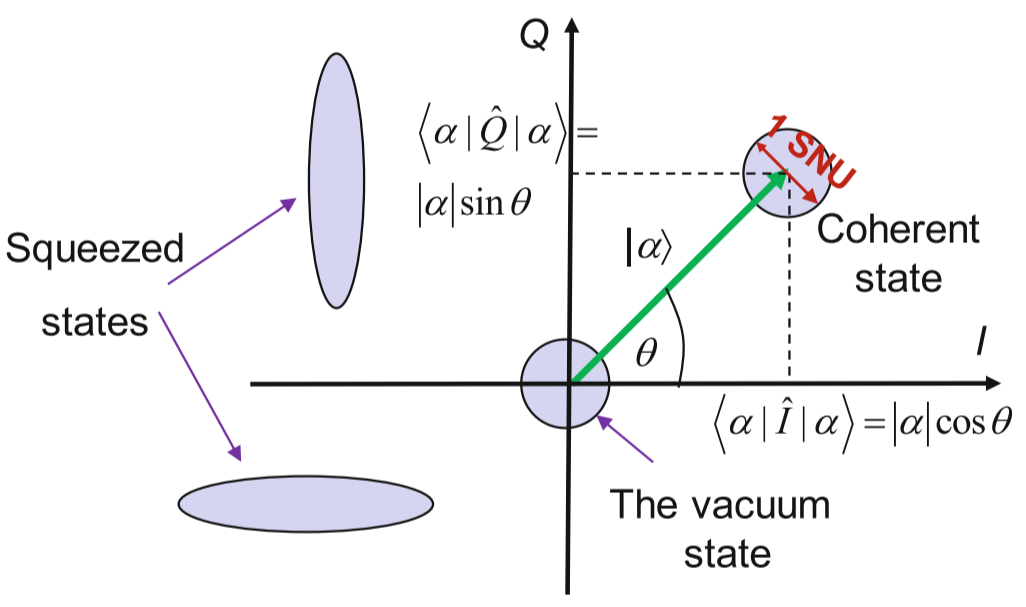
\includegraphics[width=0.8\textwidth]{chapters/figs/fig-7-13}
	\caption{تصویرسازی حالت‌های همدوس و فشرده.}
	\label{fig:7-13}
\end{figure}








در حالت‌های فشرده، مختصات $I$ با ضریب $s^{1/2}$ و مختصات $Q$ با ضریب $s^{-1/2}$ مقیاس‌بندی می‌شوند.
اکنون بیایید حالت همدوس را برحسب حالت‌های تعداد بیان کنیم. با استفاده از رابطه کامل بودن\LTRfootnote{Completeness relationship}، می‌توانیم بنویسیم:
\begin{equation}
	|\alpha\rangle = \sum_n (|n\rangle \langle n |) | \alpha \rangle = \sum_n |n\rangle \langle n|\alpha\rangle.
	\label{eq:7-81}
\end{equation}
از آنجا که حالت تعداد $|n\rangle$ را می‌توان برحسب حالت پایه\LTRfootnote{Ground state} به‌صورت زیر نمایش داد \cite{7-81}:
\begin{equation}
	|n\rangle = \frac{(a^\dagger)^n}{\sqrt{n!}} |0\rangle,
	\label{eq:7-82}
\end{equation}
ضریب تصویر را می‌توان به‌صورت زیر تعیین کرد:
\begin{equation}
	\langle n|\alpha\rangle = \langle 0 | \frac{a^n}{\sqrt{n!}} |\alpha\rangle = \frac{\alpha^n}{\sqrt{n!}} \langle 0|\alpha\rangle,
	\label{eq:7-83}
\end{equation}
و حالت همدوس پس از جایگذاری \eqref{eq:7-83} در \eqref{eq:7-81} به‌صورت زیر در می‌آید:
\begin{equation}
	|\alpha\rangle = \langle 0|\alpha\rangle \sum_n \frac{\alpha^n}{\sqrt{n!}} |n\rangle.
	\label{eq:7-84}
\end{equation}
تصویر در امتداد حالت پایه $\langle 0|\alpha\rangle$ را می‌توان از شرط هنجاریدگی\LTRfootnote{Normalization condition} تعیین کرد:
\begin{equation}
	1 = \sum_n |\langle n|\alpha\rangle|^2 = \sum_n \frac{|\langle 0|\alpha\rangle|^2 |\alpha|^{2n}}{n!} = |\langle 0|\alpha\rangle|^2 e^{|\alpha|^2},
	\label{eq:7-85}
\end{equation}
و با حل برای $\langle 0|\alpha\rangle$ به‌دست می‌آوریم:
\begin{equation}
	\langle 0|\alpha\rangle = e^{-|\alpha|^2/2},
	\label{eq:7-86}
\end{equation}
و پس از جایگذاری \eqref{eq:7-86} در \eqref{eq:7-84}، حالت همدوس به‌صورت زیر نمایش می‌یابد:
\begin{equation}
	|\alpha\rangle = e^{-|\alpha|^2/2} \sum_n \frac{\alpha^n}{\sqrt{n!}} |n\rangle.
	\label{eq:7-87}
\end{equation}
شکل مناسب دیگری را می‌توان با بیان عملگر تعداد برحسب حالت پایه، بر اساس رابطه \eqref{eq:7-82} به‌دست آورد:
\begin{equation}
	|\alpha\rangle = e^{-|\alpha|^2/2} \sum_n \frac{\alpha^n}{n!} (a^\dagger)^n |0\rangle = e^{-|\alpha|^2/2} e^{\alpha a^\dagger} |0\rangle = e^{\alpha a^\dagger - \alpha^* a} |0\rangle = D(\alpha) |0\rangle, \quad D(\alpha) = e^{\alpha a^\dagger - \alpha^* a},
	\label{eq:7-88}
\end{equation}
که در آن $D(\alpha)$ عملگر جابه‌جایی\LTRfootnote{Displacement operator} است. عملگر جابه‌جایی برای توصیف یک حالت همدوس به‌عنوان جابه‌جاییِ حالت همدوس دیگر در نمودار \lr{I-Q} استفاده می‌شود.
حالت همدوس فشرده $|\alpha, s\rangle$ را اکنون می‌توان برحسب حالت پایه به‌صورت زیر نمایش داد:
\begin{equation}
	|\alpha, s\rangle = D(\alpha) S(s) |0\rangle, \quad S(s) = e^{-\frac{1}{2}(s a^{\dagger 2} - s a^2)},
	\label{eq:7-89}
\end{equation}
که در آن $S(s)$ عملگر فشردگی\LTRfootnote{Squeezing operator} است. پارامتر فشردگی $s$ در اپتیک کوانتومی معمولاً یک عدد حقیقی است. با اعمال عملگر فشردگی بر حالت خلأ، حالت خلأ فشرده\LTRfootnote{Squeezed vacuum state} به‌دست می‌آید \cite{7-80, 7-82}:
\begin{equation}
	|0, s\rangle = (\cosh s)^{-1/2} \sum_{n=0}^{\infty} \frac{\sqrt{(2n)!}}{2^n n!} \tanh^n s |2n\rangle.
	\label{eq:7-90}
\end{equation}
هنگامی که یک بلور غیرخطی\LTRfootnote{Nonlinear crystal} با باریکه لیزری درخشان با فرکانس $2\omega$ پمپ می‌شود، فوتون‌های پمپ به جفت‌فوتون‌هایی با فرکانس $\omega$ تقسیم می‌شوند. هرگاه شرط تطبیق فاز\LTRfootnote{Phase matching} برای تقویت‌کننده پارامتری نوری\LTRfootnote{Optical parametric amplifier (OPA)} (\lr{OPA}) تباهیده برقرار باشد، خروجی برهم‌نهی از حالت‌های تعداد زوج $|2n\rangle$ خواهد بود \cite{7-78, 7-79, 7-80} که با معادله فوق همخوانی دارد. در تصویر هایزنبرگ\LTRfootnote{Heisenberg picture}، عملگر نابودی توسط تبدیل یکانی خطی بوگولیوبوف\LTRfootnote{Bogoliubov transformation} به‌صورت $a \to b = (\cosh s)a - (\sinh s)a^\dagger$ تبدیل می‌شود. از سوی دیگر، عملگرهای مربعی $\bm{x} = [x_1, x_2]^T = [I, Q]^T$ به‌صورت زیر تبدیل می‌شوند \cite{7-80}:
\begin{equation}
	\bm{x} \to \bm{x}_{\text{out}} = \begin{bmatrix} e^{-s} & 0 \\ 0 & e^s \end{bmatrix} \bm{x} = \bm{S}(s) \bm{x}, \quad \bm{S}(s) = \begin{bmatrix} e^{-s} & 0 \\ 0 & e^s \end{bmatrix}.
	\label{eq:7-91}
\end{equation}
برای عملگرهای مربعی، می‌توانیم ماتریس کوواریانس\LTRfootnote{Covariance matrix} $\bm{\Sigma} = (\Sigma_{ij})_{2 \times 2}$ را به‌صورت زیر تعریف کنیم \cite{7-80}:
\begin{equation}
	\Sigma_{ij} = \frac{1}{2} \langle \{ \Delta \hat{x}_i, \Delta \hat{x}_j \} \rangle = \frac{1}{2} \langle (\hat{x}_i \hat{x}_j + \hat{x}_j \hat{x}_i) \rangle - \langle \hat{x}_i \rangle \langle \hat{x}_j \rangle, \quad \Delta \hat{x}_i = \hat{x}_i - \langle \hat{x}_i \rangle,
	\label{eq:7-92}
\end{equation}
که در آن $\{\cdot, \cdot\}$ نشان‌دهنده پادجابه‌جاگر\LTRfootnote{Anticommutator} است. عناصر قطری ماتریس کوواریانس به‌وضوح همان واریانس‌های مؤلفه‌های مربعی هستند:
\begin{equation}
	\Sigma_{ii} = V(\hat{x}_i) = \langle (\Delta \hat{x}_i)^2 \rangle = \langle \hat{x}_i^2 \rangle - \langle \hat{x}_i \rangle^2.
	\label{eq:7-93}
\end{equation}
ماتریس کوواریانس برای تعداد دلخواهی از حالت‌های گاوسی به‌راحتی قابل تعمیم است. ماتریس کوواریانس برای حالت خلأ فشرده به‌صورت $\bm{V} = \bm{S}(s) \bm{S}(s)^T = \bm{S}(2s)$ داده می‌شود و دارای واریانس‌های متفاوتی برای مؤلفه‌های مربعی است، به‌طوری که یکی از واریانس‌ها به زیر سطح نویز شات کوانتومی فشرده شده و دیگری به بالای سطح نویز شات کوانتومی وافشرده\LTRfootnote{Antisqueezed} شده است.






\subsubsection{حالت \lr{EPR} و دست‌کاری حالت‌های فوتون}
\label{subsec:7-5-3}
زمانی که یک بلور غیرخطی\LTRfootnote{Nonlinear crystal} را در رژیم غیرتبهگن\LTRfootnote{Nondegenerate regime} پمپ می‌کنیم، بلور جفت‌فوتون‌هایی را در دو مُد مختلف تولید می‌کند که معمولاً سیگنال\LTRfootnote{Signal} و آیدلر\LTRfootnote{Idler} (کمکی) نامیده می‌شوند. این فرآیند با عنوان تبدیل پایین‌رتبه پارامتری خودبه‌خودی\LTRfootnote{Spontaneous parametric downconversion (SPDC)} (\lr{SPDC}) شناخته می‌شود \cite{7-8, 7-78, 7-79, 7-80}. با ارسال فوتون‌ها در فرکانس $\omega_p$ (سیگنال پمپ) به درون یک بلور غیرخطی، مانند $\text{KH}_2\text{PO}_4$، بتای-باریم بورات (\lr{BBO})\LTRfootnote{Beta-barium borate (BBO)} یا بلور $\text{LiNbO}_3$ با قطبش دوره‌ای (\lr{PPLN})\LTRfootnote{Periodically poled LiNbO3 (PPLN)}، جفت‌فوتون‌هایی در فرکانس‌های $\omega_s$ (سیگنال) و $\omega_i$ (آیدلر) تولید می‌کنیم که در اصل بقای انرژی $\hbar(\omega_s + \omega_i) = \hbar\omega_p$ و اصل بقای تکانه $\bm{k}_s + \bm{k}_i = \bm{k}_p$ صدق می‌کنند؛ این فرآیند در شکل \ref{fig:7-14} تصویر شده است.

\begin{figure}[ht]
	\centering
	 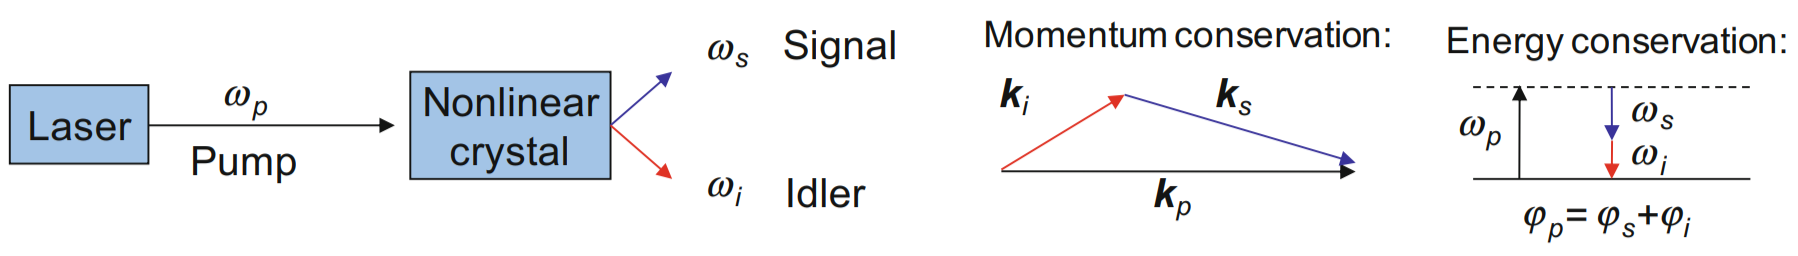
\includegraphics[width=\textwidth]{chapters/figs/fig-7-14}
	\caption{تصویرسازی فرآیند \lr{SPDC}.}
	\label{fig:7-14}
\end{figure}

یک بلور غیرخطی برای تقسیم فوتون‌ها به جفت‌فوتون‌هایی استفاده می‌شود که قانون بقای انرژی را ارضا کرده، مجموع انرژی‌ها و تکانه‌های آن‌ها برابر با انرژی و تکانه فوتون اصلی است، در حوزه فرکانس تطبیق فاز\LTRfootnote{Phase-matched} یافته‌اند و دارای قطبش‌های همبسته هستند. اگر فوتون‌ها دارای قطبش یکسان باشند، به همبستگی نوع \lr{I} تعلق دارند و در غیر این صورت، دارای قطبش‌های عمود بر هم بوده و به نوع \lr{II} تعلق دارند. از آنجا که \lr{SPDC} توسط نوسانات تصادفی خلأ تحریک می‌شود، جفت‌فوتون‌ها در لحظات زمانی تصادفی ایجاد می‌گردند. خروجی یک تبدیل‌کننده پایین‌رتبه نوع \lr{I} به‌عنوان خلأ فشرده\LTRfootnote{Squeezed vacuum} شناخته می‌شود و تنها شامل تعداد فوتون‌های زوج است. خروجی تبدیل‌کننده نوع \lr{II} به‌عنوان حالت خلأ فشرده دو-مُدی\LTRfootnote{Two-mode squeezed vacuum (TMSV)} (\lr{TMSV}) شناخته می‌شود که در ادامه توصیف می‌گردد. متناوباً، فیبر نوری بسیار غیرخطی (\lr{HNLF})\LTRfootnote{Highly nonlinear fiber (HNLF)} نیز می‌تواند به‌عنوان منبع \lr{SPDC} استفاده شود \cite{7-83, 7-84}. \lr{HNLF} از اثر اختلاط چهارموج\LTRfootnote{Four-wave mixing (FWM)} (\lr{FWM}) بهره می‌برد \cite{7-44, 7-85}. هامیلتونی توصیف‌کننده این سیستم شامل جمله دوقطبی $a^\dagger b^\dagger$ خواهد بود. عملگر یکانی گاوسی متناظر، به‌عنوان عملگر فشردگی دو-مُدی\LTRfootnote{Two-mode squeezing operator} شناخته می‌شود:
\begin{equation}
	S_2(s) = \exp\left[ -s(a^\dagger b^\dagger - ab)/2 \right],
	\label{eq:7-94}
\end{equation}
که در آن $s$ میزان فشردگی دو-مُدی را تعیین می‌کند.

در تصویر هایزنبرگ، عملگرهای مربعی $\hat{\bm{x}} = ( \hat{x}_1 \hat{x}_2 \hat{x}_3 \hat{x}_4 )^T = ( \hat{I}_a \hat{Q}_a \hat{I}_b \hat{Q}_b )^T$ به‌صورت زیر تبدیل می‌شوند \cite{7-80}:
\begin{equation}
	\hat{\bm{x}} \rightarrow \bm{\Sigma}_2(s) \hat{\bm{x}}, \quad \bm{\Sigma}_2(s) = \begin{bmatrix} \cosh s \ones & \sinh s \bm{Z} \\ \sinh s \bm{Z} & \cosh s \ones \end{bmatrix},
	\label{eq:7-95}
\end{equation}
که در آن $\ones$ ماتریس همانی و $\bm{Z} = \text{diag}(1, -1)$ ماتریس پاولی-$\bm{Z}$ است. هنگامی که $S_2(s)$ را بر دو حالت خلأ اعمال می‌کنیم، حالت \lr{TMSV} حاصل می‌شود که معمولاً به‌عنوان حالت \lr{EPR} یعنی $\rho_{EPR} = |s\rangle\langle s|_{EPR}$ شناخته می‌شود، که در آن \cite{7-80}:
\begin{equation}
	|s\rangle_{EPR} = \sqrt{1 - \lambda^2} \sum_{n=0}^{\infty} \lambda^n |n\rangle_a |n\rangle_b = \sqrt{\frac{2}{v+1}} \sum_{n=0}^{\infty} \left( \frac{v-1}{v+1} \right)^{n/2} |n\rangle_a |n\rangle_b, \quad \lambda^2 = \frac{v-1}{v+1},
	\label{eq:7-96}
\end{equation}
به‌طوری که $\lambda = \tanh(s)$ و $v = \cosh(2s)$ نشان‌دهنده واریانس مؤلفه‌های مربعی است. حالت \lr{EPR} نشان‌دهنده حالت گاوسی با میانگین صفر و ماتریس کوواریانس زیر است:
\begin{equation}
	\bm{\Sigma}_{EPR} = \begin{bmatrix} v \ones & \sqrt{v^2 - 1} \bm{Z} \\ \sqrt{v^2 - 1} \bm{Z} & v \ones \end{bmatrix}, \quad v = \cosh 2s;
	\label{eq:7-97}
\end{equation}
که در آن عناصر ماتریس کوواریانس با اعمال تعاریف روابط \eqref{eq:7-92} و \eqref{eq:7-93} بر حالت \lr{EPR} تعیین می‌شوند. حالت \lr{EPR} در رابطه \eqref{eq:7-97} مستقیماً در سیستم‌های \lr{CV-QKD} کاربرد دارد.

رایج‌ترین دستگاه‌های مورد استفاده برای دست‌کاری حالت‌های فوتون عبارتند از \cite{7-6, 7-8}: (۱) آینه‌ها، که برای تغییر جهت انتشار استفاده می‌شوند؛ (۲) جابه‌جاگرهای فاز\LTRfootnote{Phase shifters}، که برای اعمال یک جابه‌جایی فاز معین به کار می‌روند؛ و (۳) تقسیم‌کننده‌های پرتو\LTRfootnote{Beam splitters}، که برای پیاده‌سازی گیت‌های مختلف کوانتومی استفاده می‌شوند. جابه‌جاگر فاز قطعه‌ای از یک محیط شفاف، مثلاً شیشه بوروسیلیکات با ضریب شکست $n$ بزرگتر از هوا است و برای انجام عملیات زیر به کار می‌رود:
\begin{equation}
	|\psi_{\text{out}}\rangle = \begin{bmatrix} e^{j\phi} & 0 \\ 0 & 1 \end{bmatrix} |\psi\rangle; \quad \phi = kL, \quad k = n\omega/c.
	\label{eq:7-98}
\end{equation}
طرح معادل متناظر در شکل \ref{fig:7-15} نشان داده شده است.

\begin{figure}[ht]
	\centering
	 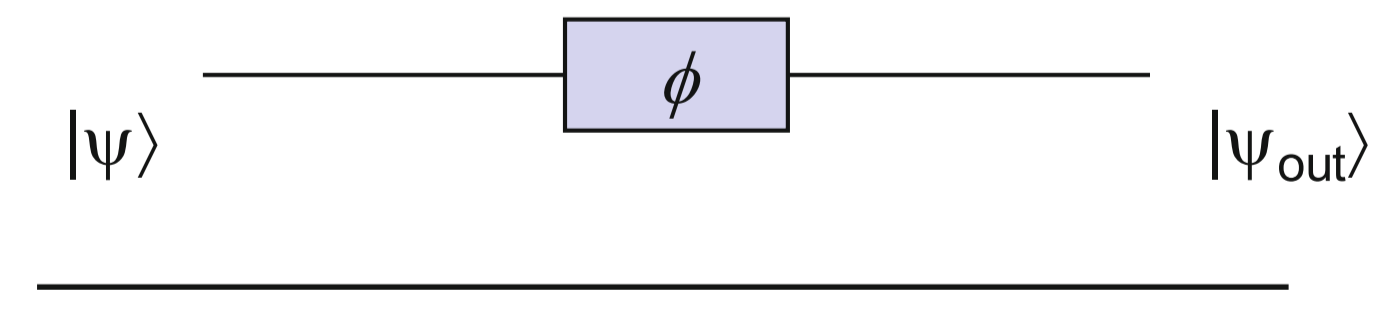
\includegraphics[width=0.5\textwidth]{chapters/figs/fig-7-15}
	\caption{طرح معادل جابه‌جاگر فاز.}
	\label{fig:7-15}
\end{figure}

تقسیم‌کننده پرتو یک قطعه شیشه با پوشش جزئی نقره است که ضریب بازتاب آن به‌صورت $R = \cos \theta$ پارامتری می‌شود. گذردهی\LTRfootnote{Transmissivity} تقسیم‌کننده پرتو به‌صورت $T = \cos^2 \theta \in [0, 1]$ داده می‌شود. در تصویر هایزنبرگ، عملگرهای نابودی مُدها توسط تبدیل بوگولیوبوف زیر تغییر می‌یابند:
\begin{equation}
	\begin{bmatrix} a \\ b \end{bmatrix} \rightarrow \begin{bmatrix} a_{\text{out}} \\ b_{\text{out}} \end{bmatrix} = \begin{bmatrix} \sqrt{T} & \sqrt{1-T} \\ -\sqrt{1-T} & \sqrt{T} \end{bmatrix} \begin{bmatrix} a \\ b \end{bmatrix} = \begin{bmatrix} \cos \theta & \sin \theta \\ -\sin \theta & \cos \theta \end{bmatrix} \begin{bmatrix} a \\ b \end{bmatrix}.
	\label{eq:7-99}
\end{equation}
تقسیم‌کننده پرتو ۵۰:۵۰ به ازای $\theta = \pi/4$ حاصل می‌شود و پیاده‌سازی آن در شکل \ref{fig:7-16} نشان داده شده است.

\begin{figure}[ht]
	\centering
	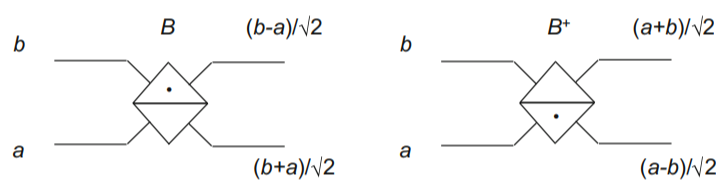
\includegraphics[width=0.7\textwidth]{chapters/figs/fig-7-16}
	\caption{تصویرسازی اصل عملکرد تقسیم‌کننده پرتو ۵۰/۵۰ (\lr{B}) و مزدوج هرمیتی آن ($\bm{B}^\dagger$).}
	\label{fig:7-16}
\end{figure}

تقسیم‌کننده پرتو بر روی دو مُد عمل می‌کند که می‌توان آن‌ها را با عملگرهای تولید (نابودی) $a^\dagger$ ($a$) و $b^\dagger$ ($b$) توصیف کرد. هامیلتونی متناظر به‌صورت زیر داده می‌شود:
\begin{equation}
	\hat{H}_{BS} = j2\theta(a^\dagger b - ab^\dagger).
	\label{eq:7-100}
\end{equation}
عملکرد تقسیم‌کننده پرتو را می‌توان با عملگر تحول به‌صورت زیر نمایش داد:
\begin{equation}
	BS(\theta) = e^{-j\hat{H}_{BS}/2} = e^{\theta(a^\dagger b - ab^\dagger)}.
	\label{eq:7-101}
\end{equation}
عملگرهای مربعی مُدها یعنی $\hat{\bm{x}} = ( \hat{x}_1 \hat{x}_2 \hat{x}_3 \hat{x}_4 )^T = ( \hat{I}_a \hat{Q}_a \hat{I}_b \hat{Q}_b )^T$ توسط تبدیل سیمپلکتیک\LTRfootnote{Symplectic transformation} زیر تغییر می‌یابند:
\begin{equation}
	\hat{\bm{x}} \rightarrow \hat{\bm{x}}_{\text{out}} = \begin{bmatrix} \sqrt{T}\ones & \sqrt{1-T}\ones \\ -\sqrt{1-T}\ones & \sqrt{T}\ones \end{bmatrix} \hat{\bm{x}}.
	\label{eq:7-102}
\end{equation}







\section{پروتکل‌های توزیع کلید کوانتومی با متغیر پیوسته (\lr{CV-QKD})}
\label{sec:7-6}
توزیع کلید کوانتومی با متغیر پیوسته\LTRfootnote{Continuous Variable (CV)-QKD} (\lr{CV-QKD}) را می‌توان با به‌کارگیری آشکارسازی هموداین\LTRfootnote{Homodyne detection}، که در آن در هر لحظه تنها یک مؤلفه مربعی\LTRfootnote{Quadrature component} (به دلیل اصل عدم قطعیت\LTRfootnote{Uncertainty principle}) اندازه‌گیری می‌شود، یا با آشکارسازی هتروداین\LTRfootnote{Heterodyne detection (HD)} (\lr{HD}) پیاده‌سازی کرد؛ در روش دوم، از یک تقسیم‌کننده پرتو\LTRfootnote{Beam splitter (BS)} (\lr{BS}) و دو فتودتکتور متعادل برای اندازه‌گیری هم‌زمان هر دو مؤلفه مربعی استفاده می‌شود، همان‌طور که در شکل \ref{fig:7-17} تصویر شده است.

\begin{figure}[ht]
	\centering
	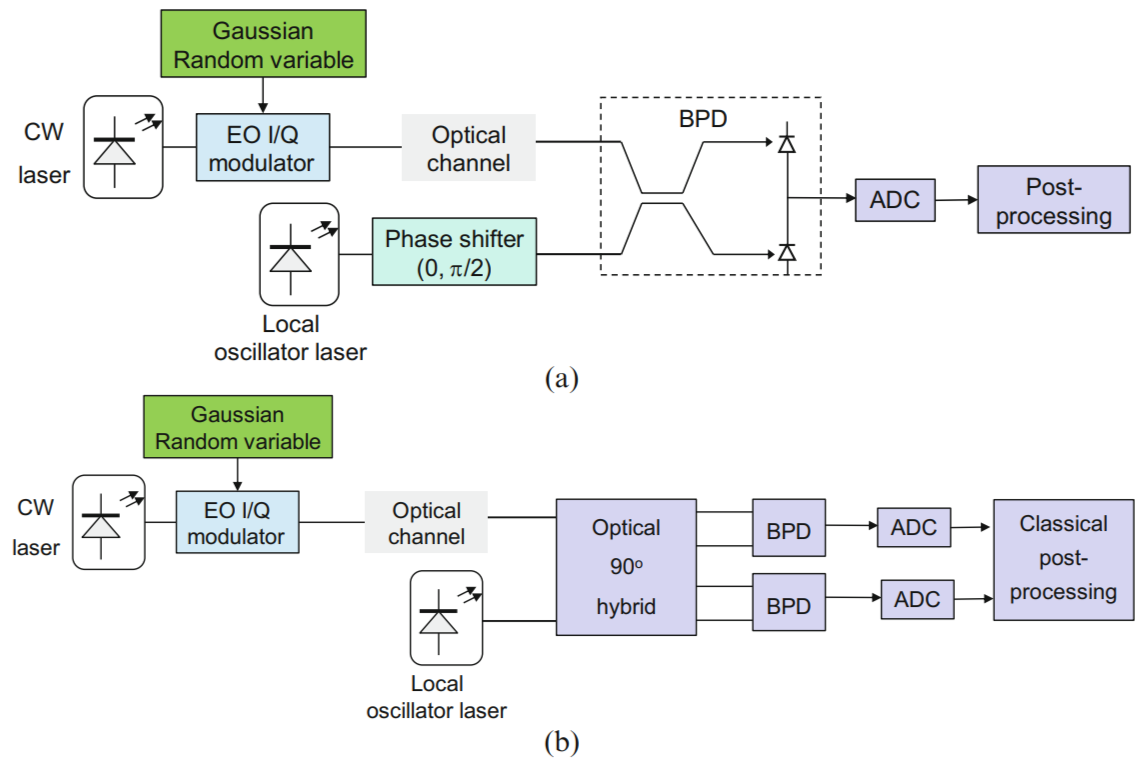
\includegraphics[width=\textwidth]{chapters/figs/fig-7-17}
	\caption{تصویرسازی پروتکل‌های \lr{CV-QKD} مبتنی بر مدولاسیون گاوسی گسسته: (الف) طرح \lr{CV-QKD} مبتنی بر آشکارسازی هموداین؛ (ب) طرح \lr{CV-QKD} مبتنی بر آشکارسازی هتروداین. \lr{ADC}: تبدیل آنالوگ به دیجیتال؛ \lr{BPD}: فتوآشکارسازی متعادل.}
	\label{fig:7-17}
\end{figure}

آشکارسازی هتروداین می‌تواند اطلاعات متقابل\LTRfootnote{Mutual information} بین آلیس و باب را در مقایسه با طرح آشکارسازی هموداین دوبرابر کند، که البته این امر به قیمت تلفات اضافی $3$ \lr{dB} ناشی از تقسیم‌کننده پرتو تمام می‌شود. به‌منظور کاهش نویز فاز لیزر، سیگنال‌های کوانتومی معمولاً همراه با یک تُن پایلوت\LTRfootnote{Pilot-tone (PT)} (\lr{PT}) پرتوانِ تسهیم‌شده در حوزه زمان ارسال می‌شوند تا پایه‌های اندازه‌گیری آلیس و باب با یکدیگر هم‌راستا گردند. برای پیاده‌سازی \lr{CV-QKD}، هم می‌توان از حالت‌های فشرده\LTRfootnote{Squeezed states} و هم از حالت‌های همدوس\LTRfootnote{Coherent states} استفاده کرد. مطالعات \lr{CV-QKD} با قضاوت از روی تعداد فزاینده مقالات مرتبط با این حوزه \cite{7-7, 7-86, 7-87, 7-88, 7-89, 7-90, 7-91, 7-92, 7-93, 7-94, 7-95, 7-96, 7-97, 7-98, 7-99, 7-100, 7-101} و به لطف سازگاری آن‌ها با فناوری‌های پیشرفته مخابرات نوری، در حال شتاب گرفتن است.

سیستم \lr{CV-QKD} هنگام استفاده از مصالحه مستقیم\LTRfootnote{Direct reconciliation}، با محدودیت تلفات $3$ \lr{dB} در گذردهی مواجه می‌شود. برای جلوگیری از این مشکل، یا از روش‌های مصالحه معکوس\LTRfootnote{Reverse reconciliation} \cite{7-86} و یا از روش‌های پس‌گزینش\LTRfootnote{Postselection} \cite{7-96} استفاده می‌شود. استراتژی‌های مختلف شنود که در بخش \ref{sec:7-4-1} بحث شد، برای سیستم‌های \lr{CV-QKD} نیز قابل اعمال هستند. نشان داده شده است که برای مدولاسیون گاوسی\LTRfootnote{Gaussian modulation}، حمله گاوسی بهینه‌ترین حمله برای هر دو نوع حملات انفرادی \cite{7-102} و حملات دسته‌جمعی \cite{7-103, 7-104} است.

\subsection{پروتکل مبتنی بر حالت‌های فشرده}
\label{subsec:7-6-1}
پروتکل‌های مبتنی بر حالت‌های فشرده از اصل عدم قطعیت هایزنبرگ بهره می‌گیرند که بیان می‌کند اندازه‌گیری هر دو مؤلفه مربعی با دقت کامل غیرممکن است. برای اعمال اطلاعات، آلیس به‌طور تصادفی انتخاب می‌کند که از درجه آزادی\LTRfootnote{Degree of freedom (DOF)} (\lr{DOF}) هم‌فاز یا مربعی استفاده کند، همان‌طور که در شکل \ref{fig:7-18} (سمت چپ) نشان داده شده است.

\begin{figure}[ht]
	\centering
	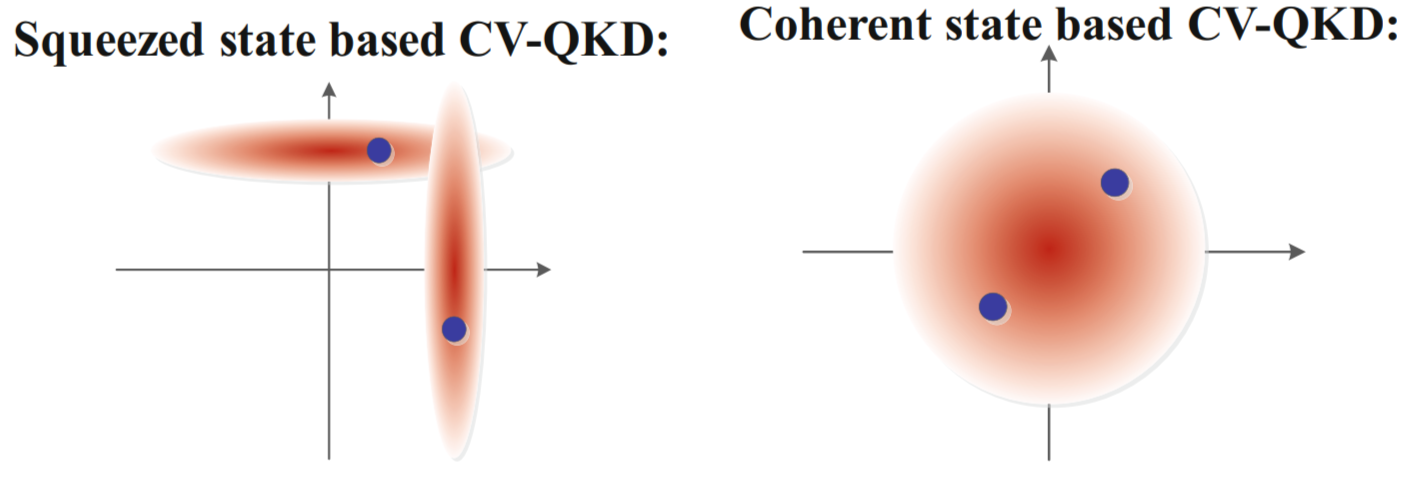
\includegraphics[width=0.9\textwidth]{chapters/figs/fig-7-18}
	\caption{تصویرسازی اصول عملکرد پروتکل‌های مبتنی بر حالت فشرده (چپ) و همدوس (راست).}
	\label{fig:7-18}
\end{figure}

در قاعده کدگذاری آلیس $I$ (زمانی که از \lr{DOF} هم‌فاز استفاده می‌شود)، حالت فشرده بر روی مؤلفه هم‌فاز (با پارامتر فشردگی $s_I < 1$) اعمال می‌شود:
\begin{equation}
	X_{A,I} \rightarrow |X_{A,I}, s_I \rangle, \quad s_I < 1, \quad X_{A,I} \sim \mathcal{N}(0, \sqrt{v_{A,I} N_0})
	\label{eq:7-103}
\end{equation}
دامنه از یک منبع گاوسی با میانگین صفر و واریانس $v_{A,I} N_0$ انتخاب می‌شود. از سوی دیگر، در قاعده کدگذاری آلیس $Q$ (زمانی که از مؤلفه مربعی استفاده می‌شود)، حالت فشرده بر روی مؤلفه مربعی (با پارامتر فشردگی $s_Q > 1$) اعمال شده و می‌توانیم بنویسیم:
\begin{equation}
	X_{A,Q} \rightarrow |jX_{A,Q}, s_Q \rangle, \quad s_Q > 1, \quad X_{A,Q} \sim \mathcal{N}(0, \sqrt{v_{A,Q} N_0})
	\label{eq:7-104}
\end{equation}
واریانس‌های حالت‌های فشرده $I$ و $Q$ به‌ترتیب برابر با $V(\hat{I}) = \sigma_I^2 N_0 = s_I N_0$ و $V(\hat{Q}) = \sigma_Q^2 N_0 = N_0/s_2$ خواهند بود (همان‌طور که در بالا شرح داده شد). در سمت گیرنده، باب به‌طور تصادفی انتخاب می‌کند که مؤلفه $I$ یا $Q$ را اندازه‌گیری کند. آلیس و باب قواعد کدگذاری به‌کار رفته برای اندازه‌گیری مؤلفه مربعی را به ازای هر حالت فشرده مبادله کرده و در فرآیند غربال‌گری، تنها مواردی را که در آن‌ها مؤلفه مربعی یکسانی را اندازه‌گیری کرده‌اند، نگه می‌دارند. بنابراین، این پروتکل بسیار شبیه به پروتکل \lr{BB84} است. سپس مصالحه اطلاعات و به‌دنبال آن تقویت حریم خصوصی انجام می‌شود.

از دیدگاه ایو، حالت‌های مخلوط متناظر زمانی که آلیس از \lr{DOF} هم‌فاز یا مربعی استفاده کرده است، به‌صورت زیر خواهد بود \cite{7-7}:
\begin{equation}
	\begin{aligned}
		\rho_I &= \int f_N(0, \sqrt{v_{A,I} N_0}) |x, s_I \rangle \langle x, s_I| dx, \\
		\rho_Q &= \int f_N(0, \sqrt{v_{A,Q} N_0}) |jQ, s_Q \rangle \langle jQ, s_Q| dx
	\end{aligned}
	\label{eq:7-105}
\end{equation}
که در آن $f_N(0, \sigma)$ توزیع گاوسی با میانگین صفر و واریانس $\sigma^2$ است. هنگامی که شرط $\rho_I = \rho_Q$ برقرار باشد، ایو نمی‌تواند تشخیص دهد که آلیس اطلاعات را روی حالت فشرده $I$ اعمال کرده است یا $Q$. بر اساس رابطه \eqref{eq:7-77}، برای اطمینان از اینکه ایو نتواند بین حالت‌های فشرده $I$ و $Q$ تمایز قائل شود، نیاز داریم که:
\begin{equation}
	(v_{A,I} + \sigma_I^2)\sigma_Q^2 = 1, \quad (v_{A,Q} + \sigma_Q^2)\sigma_I^2 = 1.
	\label{eq:7-106}
\end{equation}
با تقسیم طرفین چپ هر دو معادله، به‌دست می‌آوریم:
\begin{equation}
	\frac{(v_{A,I} + \sigma_I^2)\sigma_Q^2}{(v_{A,Q} + \sigma_Q^2)\sigma_I^2} = 1 \implies 1 + \frac{v_{A,1}}{\sigma_I^2} = 1 + \frac{v_{A,Q}}{\sigma_Q^2}.
	\label{eq:7-107}
\end{equation}
با توجه به اینکه تولید حالت‌های فشرده بسیار دشوارتر از حالت‌های همدوس است، تمرکز خود را بر پروتکل‌های \lr{CV-QKD} مبتنی بر حالت‌های همدوس معطوف می‌کنیم.








\subsection{پروتکل‌های مبتنی بر حالت‌های همدوس}
\label{sec:7-6-2}
در پروتکل‌های مبتنی بر حالت‌های همدوس\LTRfootnote{Coherent states-based protocols}، تنها یک قاعده کدگذاری برای آلیس وجود دارد:
\begin{equation}
	(X_{A,I}, X_{A,Q}) \rightarrow |X_{A,I} + jX_{A,Q} \rangle, \quad X_{A,I} \sim \mathcal{N}(0, \sqrt{v_A N_0}), \quad X_{A,Q} \sim \mathcal{N}(0, \sqrt{v_A N_0})
	\label{eq:7-108}
\end{equation}
به عبارت دیگر، آلیس به‌طور تصادفی نقطه‌ای را در فضای دو‌بعدی (\lr{I, Q}) از یک توزیع گاوسی متقارن دایره‌ای\LTRfootnote{Circular symmetric Gaussian distribution} با میانگین صفر انتخاب می‌کند، همان‌طور که در شکل \ref{fig:7-18} (راست) تصویر شده است. به‌وضوح، هر دو مؤلفه مربعی دارای عدم قطعیت یکسانی هستند. در اینجا نیز مجدداً از اصل عدم قطعیت هایزنبرگ استفاده می‌کنیم که بیان می‌دارد اندازه‌گیری هر دو مؤلفه مربعی با دقت کامل غیرممکن است. در سمت گیرنده، باب اندازه‌گیری تصادفی را روی مؤلفه $I$ یا $Q$ انجام می‌دهد؛ فرض کنید نتیجه اندازه‌گیری او با $Y_B$ نشان داده شود. وقتی باب $I$ را اندازه‌گیری می‌کند، اندازه‌گیری او ($Y_B$) با $X_{A,I}$ همبسته است. از سوی دیگر، وقتی باب $Q$ را اندازه‌گیری می‌کند، نتیجه اندازه‌گیری او ($Y_B$) با $X_{A,Q}$ همبسته است. به‌وضوح، باب قادر است با استفاده از حالت همدوس گاوسی، یک مختصات واحد از نقطه منظومه سیگنال\LTRfootnote{Signal constellation point} ارسال شده توسط آلیس را اندازه‌گیری کند. سپس باب اعلام می‌کند که در هر بازه سیگنال‌دهی کدام مؤلفه مربعی را اندازه‌گیری کرده است و آلیس مختصاتی را انتخاب می‌کند که با مؤلفه مربعی اندازه‌گیری شده توسط باب مطابقت دارد. باقی پروتکل مشابه پروتکل مبتنی بر حالت‌های فشرده است.

از دیدگاه ایو، حالت مخلوط\LTRfootnote{Mixed state} به‌صورت زیر خواهد بود:
\begin{equation}
	\rho = \int f_N(0, \sqrt{v_A N_0}) f_N(0, \sqrt{v_A N_0}) |I + jQ \rangle \langle I + jQ| dI dQ
	\label{eq:7-109}
\end{equation}
در اینجا $v_A$ واریانس مدولاسیون آلیس و $N_0$ نشان‌دهنده واریانس نوسانات حالت‌های همدوس است. برای ارسال بدون تلفات\LTRfootnote{Lossless transmission}، واریانس کل متغیر تصادفی باب به‌صورت زیر خواهد بود:
\begin{equation}
	V(Y_B) = \text{Var}(Y_B) = v_A N_0 + N_0 = (v_A + 1)N_0,
	\label{eq:7-110}
\end{equation}
که از جمله مدولاسیون آلیس $v_A N_0$ و واریانس نوسانات ذاتی حالت همدوس $N_0$ تشکیل شده است.

\subsubsection{مدل کانال همراه با تلفات و اطلاعات متقابل}
\label{subsec:7-6-2-1}
برای ارسال همراه با تلفات\LTRfootnote{Lossy transmission}، کانال را می‌توان به‌صورت یک تقسیم‌کننده پرتو با تضعیف $0 \leq T \leq 1$ مدل‌سازی کرد، همان‌طور که در شکل \ref{fig:7-19} تصویر شده است.

\begin{figure}[ht]
	\centering
	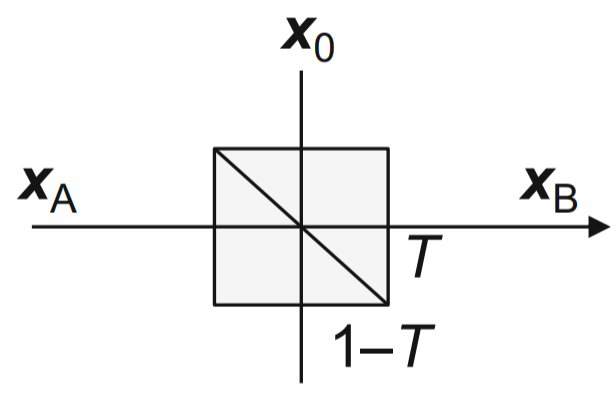
\includegraphics[width=0.8\textwidth]{chapters/figs/fig-7-19}
	\caption{تصویرسازی کانال ارسال همراه با تلفات.}
	\label{fig:7-19}
\end{figure}

از این شکل نتیجه می‌گیریم که حالت خروجی $x_B$ را می‌توان برحسب حالت ورودی $x_A$ و حالت پایه $x_0$ به‌صورت زیر نشان داد:
\begin{equation}
	x_B = \sqrt{T} x_A + \sqrt{1 - T} x_0 = \sqrt{T} (x_A + \sqrt{\chi_{\text{line}}} x_0), \quad \chi_{\text{line}} = (1 - T)/T = 1/T - 1
	\label{eq:7-111}
\end{equation}
برای ارسال همراه با تلفات، زمانی که به جای حالت‌های خلأ از مدولاسیون گاوسی حالت‌های همدوس استفاده می‌شود، رابطه قبلی باید به‌صورت زیر اصلاح گردد:
\begin{equation}
	x_B = \sqrt{T} (x_A + \sqrt{\chi_{\text{line}}} x_0), \quad \chi_{\text{line}} = (1 - T)/T + \epsilon = 1/T - 1 + \epsilon, \quad \epsilon \geq 0
	\label{eq:7-112}
\end{equation}
نخستین جمله در $\chi_{\text{line}}$ مربوط به تضعیف کانال است، در حالی که جمله دوم یعنی $\epsilon$ که معمولاً نویز اضافی\LTRfootnote{Excess noise} نامیده می‌شود، ناشی از سایر عوامل نویزی نظیر نویز فاز لیزر، عدم تعامد کامل مؤلفه‌های مربعی و غیره است. واریانس کل متغیر تصادفی باب اکنون شامل سه جمله خواهد بود:
\begin{equation*}
	V(Y_B) = \text{Var}(Y_B) = T(v_A N_0 + N_0 + \chi_{\text{line}} N_0) = T \left( \underbrace{v_A + 1}_{v} + \chi_{\text{line}} \right) N_0 = T(v + \chi_{\text{line}}) N_0,
\end{equation*}
که در آن $v = v_A + 1$ است.
اطلاعات متقابل بین آلیس و باب بر اساس فرمول شانون\LTRfootnote{Shannon's formula} را می‌توان به‌صورت زیر محاسبه کرد:
\begin{equation}
	I(A; B) \doteq I(X_A; Y_B) = \frac{1}{2} \log \left( 1 + \frac{T v_A N_0}{T(N_0 + \chi_{\text{line}} N_0)} \right) = \frac{1}{2} \log \left( 1 + \frac{v_A}{1 + \chi_{\text{line}}} \right).
	\label{eq:7-113}
\end{equation}
اطلاعات ایو در طرح‌های \lr{CV-QKD} توسط استراتژی مصالحه\LTRfootnote{Reconciliation strategy} تعیین می‌شود.







\subsubsection{مصالحه اطلاعات}
\label{subsec:7-6-3}
در مصالحه مستقیم\LTRfootnote{Direct reconciliation}، کلید بر اساس متغیر تصادفی آلیس $X_A$ تعیین می‌شود (و باب عملیات تصحیح خطا را روی دنباله خود انجام می‌دهد)، به‌طوری که کسر مخفی\LTRfootnote{Secret fraction} به‌صورت زیر داده می‌شود:
\begin{equation}
	r = I(X_A; Y_B) - I(X_A; Z)
	\label{eq:7-114}
\end{equation}
باب و ایو نمی‌توانند هر دو تمام اطلاعات مربوط به عناصر کلیدی پروتکل را به‌دست آورند؛ واریانس باب روی $\hat{I}$ و ایو روی $\hat{Q}$ در رابطه عدم قطعیت $\chi_{\text{line}}\chi_E \geq 1$ صدق می‌کند، به‌طوری که اطلاعات متقابل بین آلیس و ایو به‌صورت زیر به‌دست می‌آید:
\begin{equation}
	I(A; E) = \frac{1}{2} \log \left( 1 + \frac{v_A}{1 + \underbrace{\chi_E}_{1/\chi_{\text{line}}}} \right) = \frac{1}{2} \log \left( 1 + \frac{v_A}{1 + 1/\chi_{\text{line}}} \right).
	\label{eq:7-115}
\end{equation}
با جایگذاری روابط \eqref{eq:7-113} و \eqref{eq:7-115} در \eqref{eq:7-114}، خواهیم داشت:
\begin{equation}
	r = \frac{1}{2} \log \left( 1 + \frac{v_A}{1 + \chi_{\text{line}}} \right) - \frac{1}{2} \log \left( 1 + \frac{v_A}{1 + 1/\chi_{\text{line}}} \right) = \frac{1}{2} \log \left[ \frac{1 + \chi_{\text{line}} + v_A}{1 + \chi_{\text{line}} + v_A \chi_{\text{line}}} \right].
	\label{eq:7-116}
\end{equation}
به ازای $T = 1/2$، مقدار $\chi_{\text{line}} = 1$ شده و آرگومان لگاریتم برابر با $1$ می‌گردد که در نتیجه $r$ صفر می‌شود. بنابراین، در طرح مصالحه مستقیم، تضعیف کانال باید کمتر از $3$ \lr{dB} باشد.

در مصالحه معکوس\LTRfootnote{Reverse reconciliation}، کلید از روی اندازه‌گیری‌های باب تعیین می‌شود (و آلیس تصحیح خطا را روی دنباله خود انجام می‌دهد)، به‌طوری که کسر مخفی به‌صورت زیر است:
\begin{equation}
	r = I(X_B; Y_A) - I(X_B; Z),
	\label{eq:7-117}
\end{equation}
در حالی که اطلاعات متقابل بین باب و آلیس توسط رابطه \eqref{eq:7-113} تعیین می‌شود، اما به شکلی متفاوت بازنویسی می‌گردد:
\begin{equation}
	I(X_B; Y_A) = \frac{1}{2} \log \left( \frac{\overbrace{v_A + 1}^v + \chi_{\text{line}}}{1 + \chi_{\text{line}}} \right) = \frac{1}{2} \log \left( \frac{v + \chi_{\text{line}}}{1 + \chi_{\text{line}}} \right), \quad v = v_A + 1.
	\label{eq:7-118}
\end{equation}
استراتژی شنود گاوسی بهینه بر اساس ماشین کپی‌کننده درهم‌تننده\LTRfootnote{Entangling cloning machine} است که در شکل \ref{fig:7-20} نشان داده شده است.

\begin{figure}[ht]
	\centering
	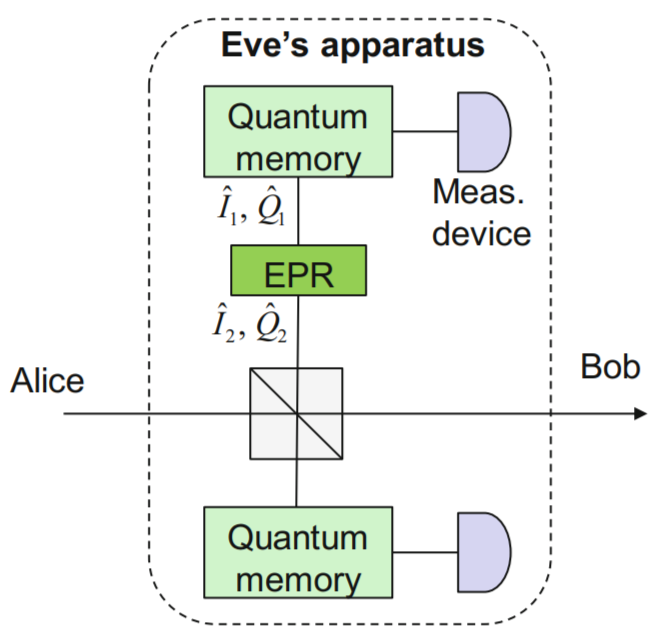
\includegraphics[width=0.6\textwidth]{chapters/figs/fig-7-20}
	\caption{استراتژی شنود گاوسی بهینه بر پایه ماشین کپی‌کننده درهم‌تننده.}
	\label{fig:7-20}
\end{figure}

در دستگاه ایو، از منبع \lr{EPR} استفاده می‌شود که یک نیمه آن توسط ایو در حافظه کوانتومی\LTRfootnote{Quantum memory (QM)} (\lr{QM}) نگه داشته شده و نیمه دیگر توسط یک تقسیم‌کننده پرتو به کانال آلیس-باب تزریق می‌شود. این تقسیم‌کننده پرتو همچنین بخشی از حالت همدوس ارسال شده توسط آلیس را استخراج کرده و ایو آن را در یک \lr{QM} دیگر ذخیره می‌کند تا زمانی که باب اعلام کند در هر بازه سیگنال‌دهی کدام مؤلفه مربعی را اندازه‌گیری کرده است. فرض کنید مؤلفه‌های مربعی بالایی (نگهداری شده توسط ایو در \lr{QM}) با $I_1, Q_1$ و مؤلفه‌های تزریق شده به کانال آلیس-باب با $I_2, Q_2$ نشان داده شوند. به‌وضوح، ایو می‌تواند به‌طور هم‌زمان مؤلفه‌های ارسالی برای باب را با مؤلفه‌های موجود در \lr{QM} خود همبسته کند، چرا که $[I_1 - I_2, Q_1 + Q_2] = 0$ است. از سوی دیگر، با توجه به اینکه $[I_1 - I_2, Q_2] = 2jN_0$ است، همبستگی بین دو مؤلفه هم‌فاز نمی‌تواند کامل باشد و طبق اصل عدم قطعیت داریم $\langle (I_1 - I_2)^2 \rangle \langle Q_2^2 \rangle \geq N_0^2$؛ رابطه مشابهی برای همبستگی‌ها در مؤلفه مربعی $Q$ نیز برقرار است. به‌طور خلاصه، می‌توانیم اصل عدم قطعیت را (در واحد نویز شات\LTRfootnote{Shot noise unit (SNU)}) به‌صورت زیر نمایش دهیم \cite{7-46}:
\begin{equation}
	v_{B|E} v_{B|A} \geq 1,
	\label{eq:7-119}
\end{equation}
که در آن $B$ نماینده هر یک از مؤلفه‌های مربعی باب است.
ما همچنین از تعریف زیر برای واریانس شرطی $v_{X|Y}$ استفاده می‌کنیم که مقدار عدم قطعیت روی $X$ را پس از انجام اندازه‌گیری روی $Y$ کمی‌سازی می‌کند \cite{7-46, 7-105}:
\begin{equation}
	v_{X|Y} = \langle x^2 \rangle - |\langle xy \rangle|^2 / \langle y^2 \rangle.
	\label{eq:7-120}
\end{equation}
آلیس از تخمین‌گرهای $(I_A, Q_A)$ برای میدانی که ارسال می‌کند $(I_A + A_I, Q_A + A_Q)$ استفاده می‌کند، که در آن $\langle A_I^2 \rangle = \langle A_Q^2 \rangle = sN_0$ است و $s > 1/v$ پارامتری است که او برای اطمینان از سازگاری با اصل عدم قطعیت اعمال می‌کند. با محاسبه $\langle Q_A^2 \rangle = (v - s)N_0$، $\langle Q_B^2 \rangle = T(v + \chi_{\text{line}})N_0$ و $\langle Q_A Q_B \rangle = \sqrt{T} \langle Q_A^2 \rangle$ و جایگذاری در رابطه \eqref{eq:7-120}، واریانس شرطی زیر حاصل می‌شود \cite{7-105}:
\begin{equation}
	v_{B|A} = \langle Q_B^2 \rangle - |\langle Q_B Q_A \rangle|^2 / \langle Q_A^2 \rangle = T(s + \chi_{\text{line}})N_0.
	\label{eq:7-121}
\end{equation}
محدودیت $s > 1/v$ رابطه $v_{B|A} \geq T(1/v + \chi_{\text{line}})N_0$ را برای واریانس شرطی به‌دست می‌دهد و از اصل عدم قطعیت \eqref{eq:7-119}، واریانس شرطی زیر برای باب به شرط اندازه‌گیری‌های ایو حاصل می‌شود:
\begin{equation}
	v_{B|E} \geq N_0^2 / [T(1/v + \chi_{\text{line}})N_0].
	\label{eq:7-122}
\end{equation}
اکنون می‌توانیم اطلاعات متقابل بین باب و ایو را به‌صورت زیر محاسبه کنیم \cite{7-105}:
\begin{equation}
	I(B; E) = \frac{1}{2} \log \left( \frac{v_B}{v_{B|E}} \right) = \frac{1}{2} \log \left( \frac{T(v + \chi_{\text{line}})N_0}{\frac{N_0}{T(1/v + \chi_{\text{line}})}} \right) = \frac{1}{2} \log [T^2(v + \chi_{\text{line}})(1/v + \chi_{\text{line}})].
	\label{eq:7-123}
\end{equation}
پس از جایگذاری \eqref{eq:7-118} و \eqref{eq:7-123} در \eqref{eq:7-117}، عبارت کسر مخفی به‌دست می‌آید:
\begin{equation}
	r = I(B; A) - I(B; E) = \frac{1}{2} \log \left( \frac{v + \chi_{\text{line}}}{1 + \chi_{\text{line}}} \right) - \frac{1}{2} \log [T^2 (v + \chi_{\text{line}})(1/v + \chi_{\text{line}})],
	\label{eq:7-124}
\end{equation}
که پس از بازآرایی به‌صورت زیر در می‌آید:
\begin{equation}
	r = -\frac{1}{2} \log [(1 + \chi_{\text{line}}) T^2 (1/v + \chi_{\text{line}})] > 0, \quad T > 0.
	\label{eq:7-125}
\end{equation}
به‌وضوح، تا زمانی که $T > 0$ باشد، کسر مخفی نیز مثبت است.

تا اینجا، ما از آشکارسازی ناقص باب و نویز الکتریکی صرف‌نظر کردیم. با ارجاع به ورودی باب (یا به‌طور معادل خروجی کانال)، می‌توانیم واریانس نویز آشکارساز معادلِ باب را به‌صورت زیر نشان دهیم:
\begin{equation}
	\chi_{\text{det}} = \frac{d(1 + v_{el}) - \eta}{\eta},
	\label{eq:7-126}
\end{equation}
که در آن برای آشکارسازی هموداین $d=1$ و برای آشکارسازی هتروداین $d=2$ است. پارامتر $\eta$ نشان‌دهنده بازدهی آشکارسازی و $v_{el}$ نشان‌دهنده واریانس نویز الکتریکی معادل است. واریانس نویز کل را می‌توان با جمع کردن واریانس نویز کانال و نویز آشکارسازی تعیین کرد، که با ارجاع به ورودی کانال به‌صورت زیر بیان می‌شود:
\begin{equation}
	\chi_{\text{total}} = \chi_{\text{line}} + \frac{\chi_{\text{det}}}{T} = \frac{1 - T}{T} + \epsilon + \frac{d(1 + v_{el}) - \eta}{T\eta}.
	\label{eq:7-127a}
\end{equation}
هنگام ارجاع به خروجی کانال، واریانس نویز کل در سمت باب به‌صورت زیر تعیین می‌شود:
\begin{equation}
	\begin{aligned}
		\chi_{\text{total,Bob}} &= T\eta \left( \chi_{\text{line}} + \frac{\chi_{\text{det}}}{T} \right) = T\eta \frac{1 - T}{T} + T\eta\epsilon + T\eta \frac{d(1 + v_{el}) - \eta}{T\eta} \\
		&= \eta(1 - T) + T\eta\epsilon + d(1 + v_{el}) - \eta.
		\label{eq:7-127b}
	\end{aligned}
\end{equation}
عبارت متناظر برای کسر مخفی \eqref{eq:7-125} باید به‌صورت زیر اصلاح شود:
\begin{equation}
	r = -\frac{1}{2} \log [(1 + \chi_{\text{total}}) (T\eta)^2 (1/v + \chi_{\text{total}})].
	\label{eq:7-128}
\end{equation}









\subsubsection{پیاده‌سازی پروتکل GG02}
\label{subsec:7-6-4}
در این بخش، یک پیکربندی معمول برای سیستم \lr{CV-QKD} \lr{GG02} را شرح می‌دهیم که به نام نویسندگان آن، گروس‌هانز\LTRfootnote{Grosshans} و گرنژیه\LTRfootnote{Grangier} که آن را در سال ۲۰۰۲ پیشنهاد دادند، نام‌گذاری شده است \cite{7-89} (همچنین ببینید \cite{7-7}). طرح متناظر در شکل \ref{fig:7-21} نشان داده شده است.

\begin{figure}[ht]
	\centering
	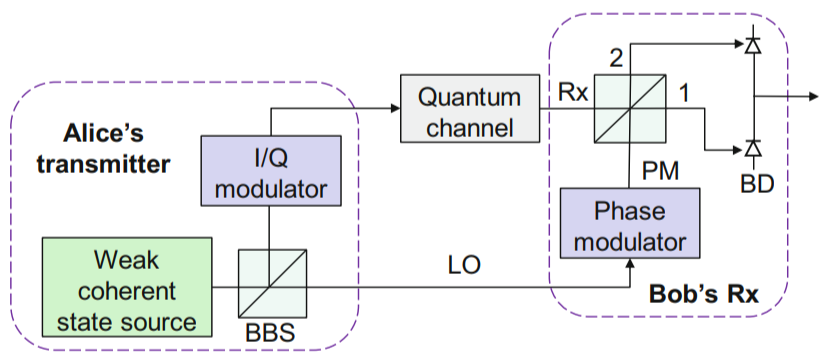
\includegraphics[width=0.8\textwidth]{chapters/figs/fig-7-21}
	\caption{پیکربندی سیستم \lr{CV-QKD} \lr{GG02}. \lr{LO}: سیگنال نوسان‌ساز محلی (مرجع)؛ \lr{BBS}: تقسیم‌کننده پرتو متعادل؛ \lr{BD}: آشکارساز متعادل.}
	\label{fig:7-21}
\end{figure}

آلیس از یک منبع حالت همدوس ضعیف\LTRfootnote{Weak coherent state (WCS)} (\lr{WCS}) مانند باریکه لیزرِ به‌قدر کافی تضعیف‌شده برای به‌دست آوردن حالت گاوسی استفاده می‌کند و در ادامه از یک تقسیم‌کننده پرتو متعادل\LTRfootnote{Balanced beam splitter (BBS)} (\lr{BBS}) برای تقسیم سیگنال به دو بخش بهره می‌برد. خروجی بالایی \lr{BS} توسط مدولاتور \lr{I/Q} مدوله می‌شود تا نقطه منظومه\LTRfootnote{Constellation point} را در مکان مورد نظر در فضای \lr{I-Q} قرار داده و واریانس آلیس $v_A$ را کنترل کند. خروجی دوم \lr{BBS} برای ارسال سیگنال مرجع نوسان‌ساز محلی\LTRfootnote{Local oscillator (LO)} (\lr{LO}) برای باب استفاده می‌شود. تعداد فوتون‌ها در خروجی‌های ۱ و ۲ از \lr{BS} گیرنده را می‌توان به‌صورت زیر بیان کرد:
\begin{equation}
	N_1 = \frac{1}{2} (a_{PM}^\dagger + a_{Rx}^\dagger)(a_{PM} + a_{Rx}), \quad N_2 = \frac{1}{2} (a_{PM}^\dagger - a_{Rx}^\dagger)(a_{PM} - a_{Rx}),
	\label{eq:7-129}
\end{equation}
که در آن عملگرهای تولید (نابودی) در ورودی‌های \lr{Rx} و \lr{PM} از \lr{BS} گیرنده به‌ترتیب با $a_{Rx}^\dagger (a_{Rx})$ و $a_{PM}^\dagger (a_{PM})$ نشان داده شده‌اند. عملگر خروجی آشکارساز متعادل\LTRfootnote{Balanced detector (BD)} (\lr{BD})، با فرض پاسخ‌دهی فتودیود\LTRfootnote{Photodiode responsivity} $P_{\text{ph}} = 1 A/W$، به‌صورت زیر داده می‌شود:
\begin{equation}
	\hat{i}_{BD} = 4N_0 (N_1 - N_2) = 4N_0 (a_{PM}^\dagger a_{Rx} + a_{Rx}^\dagger a_{PM}).
	\label{eq:7-130}
\end{equation}
عملگر نابودیِ خروجی مدولاسیون فاز را می‌توان به‌صورت $a_{PM} = |\alpha| e^{j\theta} \ones / (2\sqrt{N_0})$ نمایش داد و پس از جایگذاری در رابطه (6.162) به‌دست می‌آوریم:
\begin{equation}
	\hat{i}_{BD} = 4N_0 \left( \frac{|\alpha| e^{-j\theta}}{2\sqrt{N_0}} a_{Rx} + \frac{|\alpha| e^{j\theta}}{2\sqrt{N_0}} a_{Rx}^\dagger \right) = 2 |\alpha| \sqrt{N_0} (e^{j\theta} a_{Rx}^\dagger + e^{-j\theta} a_{Rx}).
	\label{eq:7-131}
\end{equation}
در غیاب ایو، عملگر نابودی سیگنال دریافتی به‌صورت $a_{Rx} = (I, Q) \ones / (2\sqrt{N_0})$ خواهد بود که پس از جایگذاری در رابطه (6.163) منجر به نتیجه زیر می‌شود:
\begin{equation}
	\begin{aligned}
		\hat{i}_{BD} &= |\alpha| [ (\cos \theta, \sin \theta) \ones \cdot (\hat{I}, -Q \hat{Q}) + (\cos \theta, \sin \theta) \ones \cdot (\hat{I}, Q \hat{Q}) ] \\
		&= |\alpha| (\cos \theta \cdot I \hat{I} + \sin \theta \cdot Q \hat{Q}).
		\label{eq:7-132}
	\end{aligned}
\end{equation}
باب مؤلفه هم‌فاز $I$ را با انتخاب $\theta = 0$ برای به‌دست آوردن $|\alpha|I$ و مؤلفه مربعی $Q$ را با تنظیم $\theta = \pi/2$ برای به‌دست آوردن $|\alpha|Q$ اندازه‌گیری می‌کند.

واریانس اندازه‌گیری باب دارای مؤلفه‌های زیر است: (۱) واریانس سیگنال، (۲) نوسانات ذاتی $N_0$، (۳) نویز کانال $\chi_{\text{line}} N_0$، (۴) نویز ناشی از آشکارسازی هموداین ناقص $\chi_{\text{homodyne}} N_0 = (1 - \eta)N_0 / \eta$، و (۵) نویز الکترونیکی $v_{el} N_0$؛ بنابراین می‌توانیم بنویسیم:
\begin{equation}
	\chi_{\text{total}} N_0 = \left[ \chi_{\text{line}} + \frac{\chi_{\text{homodyne}} + \overbrace{v_{el}/\eta}^{\chi_{\text{el}}}}{T_{\text{line}}} \right] N_0.
	\label{eq:7-133}
\end{equation}
از روی واریانس‌های سیگنال‌های آلیس و باب $v_A N_0 = \text{Var}(X_A)$ و $\text{Var}(X_B)$ و همچنین ضریب همبستگی $\gamma(X_A, X_B)$، می‌توانیم مقادیر زیر را تعیین کنیم \cite{7-7}:
\begin{equation}
	v_A = \text{Var}(X_A)/N_0, \quad T_{\text{line}} = \gamma^2 \text{Var}(Y_B) / \text{Var}(X_A), \quad \chi_{\text{total}} + 1 = \text{Var}(X_A)(\gamma^{-2} - 1)/N_0.
	\label{eq:7-134}
\end{equation}
اطلاعات متقابل برای کانال آلیس-به-ایو به‌صورت زیر داده می‌شود:
\begin{equation}
	I(A; E) = \frac{1}{2} \log \left( 1 + \frac{v_A}{1 + 1/\chi_{BE}} \right),
	\label{eq:7-135}
\end{equation}
که در اصل همان رابطه \eqref{eq:7-115} است. از سوی دیگر، اطلاعات متقابل برای کانال باب-به-ایو به‌صورت زیر خواهد بود \cite{7-7, 7-106, 7-107}:
\begin{equation}
	I(B; E) = \frac{1}{2} \log \left\{ \frac{T_{\text{line}} T_{\text{extra}} (v + \chi_{\text{total}})}{\chi_{BB} T_{\text{line}} + 1 / [T_{\text{line}} T_{\text{extra}} (1/v + \chi_{BE})]} \right\},
	\label{eq:7-136}
\end{equation}
که نشان‌دهنده تعمیمی از رابطه \eqref{eq:7-123} است. برای یک \textit{رویکرد پارانوئید}\LTRfootnote{Paranoid approach} (زمانی که نویزهای آشکارسازی توسط ایو کنترل می‌شوند)، باید پارامترهای معادلات بالا را به‌صورت زیر تنظیم کنیم \cite{7-7, 7-106, 7-107}:
\begin{equation}
	T_{\text{extra}} = T_{\text{homodyne}}, \quad \chi_{BE} = \chi_{\text{total}}, \quad \chi_{BB} = 0.
	\label{eq:7-137}
\end{equation}
از سوی دیگر، برای یک \textit{رویکرد واقع‌گرایانه}\LTRfootnote{Realistic approach} (زمانی که ایو نمی‌تواند نویزهای آشکارسازی را کنترل کند)، پارامترهای رابطه (6.167) را به‌صورت زیر قرار می‌دهیم \cite{7-7, 7-106, 7-107}:
\begin{equation}
	T_{\text{extra}} = 1, \quad \chi_{BE} = \chi_{\text{line}}, \quad \chi_{BB} = (\chi_{\text{homodyne}} + \chi_{el})/T_{\text{line}}.
	\label{eq:7-138}
\end{equation}
برای مصالحه مستقیم، می‌توانیم کسر مخفی را با $r = I(A; B) - I(A; E)$ محاسبه کنیم. از طرفی، برای مصالحه معکوس، کسر مخفی توسط $r = I(B; A) - I(B; E)$ قابل محاسبه است.









\subsubsection{حملات دسته‌جمعی}
\label{subsec:7-6-5}
در این بخش، به‌اختصار نحوه محاسبه کسر مخفی\LTRfootnote{Secret fraction} برای طرح \lr{CV-QKD} مبتنی بر آشکارسازی هموداینِ حالت همدوس را در شرایطی که ایو از حمله دسته‌جمعی گاوسی\LTRfootnote{Gaussian collective attack} \cite{7-90, 7-103, 7-104} استفاده می‌کند (که به عنوان بهینه‌ترین حالت برای مدولاسیون گاوسی شناخته می‌شود)، شرح می‌دهیم. این حمله به‌طور کامل با تخمین ماتریس کوواریانس\LTRfootnote{Covariance matrix} $\bm{\Sigma}_{AB}$ توسط آلیس و باب مشخص می‌شود که بر اساس رابطه \eqref{eq:7-97} و واریانس مؤلفه هم‌فاز باب که پیش‌تر تعیین شد ($V(\hat{I}) = T\eta(v + \chi_{\text{total}})$)، به‌صورت زیر نمایش می‌یابد:
\begin{equation}
	\bm{\Sigma}_{AB} = \begin{bmatrix} v\ones & \sqrt{T\eta(v^2 - 1)}\bm{Z} \\ \sqrt{T\eta(v^2 - 1)}\bm{Z} & T\eta(v + \chi_{\text{total}})\ones \end{bmatrix}, \quad v = v_A + 1.
	\label{eq:7-139}
\end{equation}
مانند قبل، فرض می‌کنیم $v = v_A + 1$ است که در آن $v_A$ واریانس (نرمالیزه شده) مدولاسیون گاوسی آلیس، $T$ گذردهی کانال، $\eta$ بازدهی آشکارسازی و $\chi_{\text{total}}$ مطابق رابطه \eqref{eq:7-127a} تعریف شده است.

هنگامی که از مصالحه معکوس\LTRfootnote{Reverse reconciliation} استفاده می‌شود، کسر مخفی به‌صورت زیر داده می‌شود:
\begin{equation}
	r = \beta I(A; B) - \chi(B; E),
	\label{eq:7-140}
\end{equation}
که در آن $\beta$ بازدهی مصالحه\LTRfootnote{Reconciliation efficiency} و $I(A; B)$ اطلاعات متقابل بین آلیس و باب است که به همان شیوه حملات انفرادی تعیین می‌شود:
\begin{equation}
	I(A; B) = \frac{d}{2} \log_2 \left( \frac{v + \chi_{\text{total}}}{1 + \chi_{\text{total}}} \right), \quad d = \begin{cases} 1, & \text{آشکارسازی هموداین} \\ 2, & \text{آشکارسازی هتروداین} \end{cases}
	\label{eq:7-141}
\end{equation}
اطلاعات هولِوو\LTRfootnote{Holevo information} بین باب و ایو که با $\chi(B; E)$ نشان داده می‌شود، طبق مراجع \cite{7-90, 7-103, 7-104} به‌صورت زیر تعیین می‌گردد:
\begin{equation}
	\chi(B; E) = g\left(\frac{\lambda_1 - 1}{2}\right) + g\left(\frac{\lambda_2 - 1}{2}\right) - g\left(\frac{\lambda_3 - 1}{2}\right) - g\left(\frac{\lambda_4 - 1}{2}\right),
	\label{eq:7-142}
\end{equation}
که در آن $g(x) = (x + 1)\log_2(x + 1) - x\log_2 x$ آنتروپی یک حالت گرمایی\LTRfootnote{Thermal state} با میانگین تعداد فوتون $x$ است. پارامترهای $\lambda$ طبق مراجع \cite{7-90, 7-108} به‌صورت زیر تعریف می‌شوند:
\begin{equation}
	\begin{aligned}
		\lambda_{1,2} &= \sqrt{\frac{1}{2} (A \pm \sqrt{A^2 - 4B})}, \quad \lambda_{3,4} = \sqrt{\frac{1}{2} (C \pm \sqrt{C^2 - 4D})}, \\
		A &= v^2(1 - 2T) + 2T + T^2(v + \chi_{\text{line}})^2, \quad B = T^2(1 + v\chi_{\text{line}})^2.
	\end{aligned}
	\label{eq:7-143}
\end{equation}
پارامترهای $C$ و $D$ برای آشکارسازی هموداین و هتروداین متفاوت هستند \cite{7-90, 7-108}:
\begin{equation}
	C = \begin{cases} 
		\frac{A\chi_{\text{homodyne}} + v\sqrt{B} + T(v + \chi_{\text{line}})}{T(v + \chi_{\text{total}})}, & \text{آشکارسازی هموداین} \\ 
		\frac{A\chi_{\text{het}}^2 + B + 1 + 2\chi_{\text{het}}[v\sqrt{B} + T(v + \chi_{\text{line}})] + 2T(v^2 - 1)}{T^2(v + \chi_{\text{total}})^2}, & \text{آشکارسازی هتروداین}
	\end{cases}
	\label{eq:7-144}
\end{equation}
\begin{equation}
	D = \begin{cases} 
		\sqrt{B} \frac{v + \chi_{\text{homodyne}}\sqrt{B}}{T(v + \chi_{\text{total}})}, & \text{آشکارسازی هموداین} \\ 
		\left( \frac{v + \chi_{\text{het}}\sqrt{B}}{T(v + \chi_{\text{total}})} \right)^2, & \text{آشکارسازی هتروداین}
	\end{cases}
	\label{eq:7-145}
\end{equation}








\section{پروتکل‌های مستقل از دستگاه اندازه‌گیری (\lr{MDI})}
\label{sec:7-7}
در پروتکل‌های مستقل از دستگاه اندازه‌گیری\LTRfootnote{Measurement-device-independent (MDI) protocols} (\lr{MDI}) \cite{7-109, 7-110, 7-111, 7-112, 7-113}، آلیس و باب از طریق یک کانال کوانتومی (مانند یک پیوند \lr{FSO} یا فیبر نوری) به شخص ثالثی به نام چارلی\LTRfootnote{Charlie} متصل می‌شوند. همان‌طور که در شکل \ref{fig:7-22} برای پیکربندی سیستم \lr{MDI-QKD} تصویر شده است، آشکارسازهای تک-فوتون در سمت چارلی قرار دارند.

\begin{figure}[ht]
	\centering
	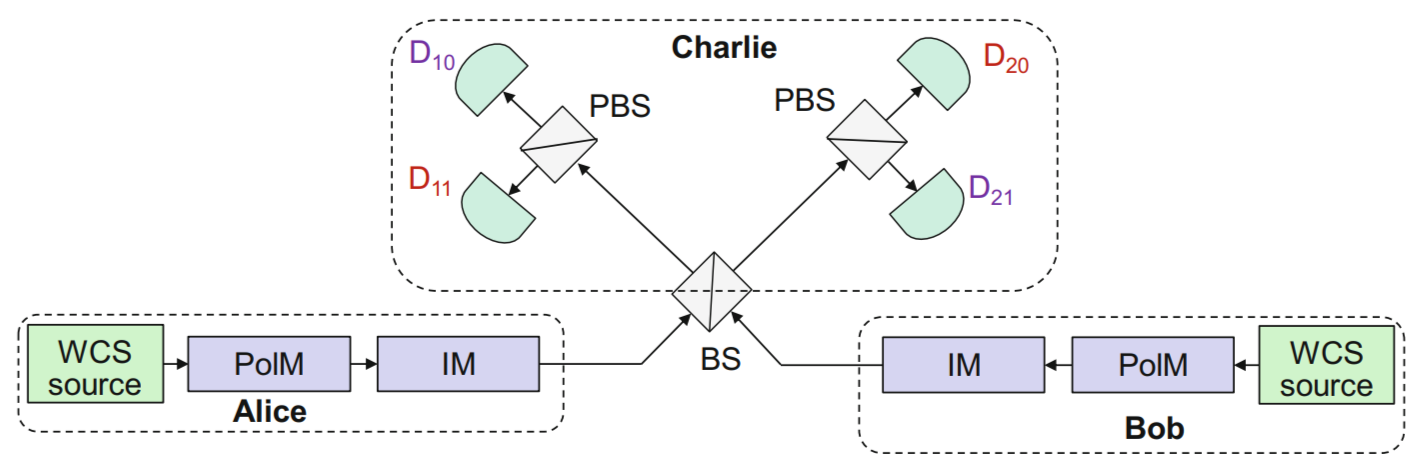
\includegraphics[width=0.8\textwidth]{chapters/figs/fig-7-22}
	\caption{پیکربندی سیستم \lr{MDI-QKD}. \lr{PolM}: مدولاتور قطبش (برای تولید یکی از چهار حالت قطبش $|0\rangle, |1\rangle, |+\rangle, |-\rangle$ استفاده می‌شود)؛ \lr{IM}: مدولاتور شدت (برای تولید حالت‌های سیگنال و فریب با شدت‌های مختلف استفاده می‌شود).}
	\label{fig:7-22}
\end{figure}

نسخه ساده‌شده این پروتکل در ادامه این بخش شرح داده می‌شود. آلیس و باب منابع تک-فوتونی در اختیار دارند و به‌طور تصادفی یکی از چهار حالت $|0\rangle, |1\rangle, |+\rangle, |-\rangle$ را برای ارسال به چارلی انتخاب می‌کنند. چارلی اندازه‌گیری حالت بل\LTRfootnote{Bell state measurement (BSM)} (\lr{BSM}) جزئی را با کمک یک تقسیم‌کننده پرتو انجام داده و رویدادهایی را اعلام می‌کند که در آن‌ها نتیجه اندازه‌گیری منجر به یکی از حالت‌های $|\psi^-\rangle = 2^{-1/2} (|0\rangle_A|1\rangle_B - |1\rangle_A|0\rangle_B)$ یا $|\psi^+\rangle = 2^{-1/2} (|0\rangle_A|1\rangle_B + |1\rangle_A|0\rangle_B)$ شده است. یک \lr{BSM} موفق متناظر با مشاهداتی است که در آن‌ها دقیقاً دو آشکارساز (با قطبش‌های متعامد) به‌صورت زیر تحریک شوند:
\begin{itemize}
	\item کلیک‌های هم‌زمان روی آشکارسازهای $D_{10}$ و $D_{21}$ (یا $D_{11}$ و $D_{20}$)، تصویر شدن بر روی حالت بل $|\psi^-\rangle$ را شناسایی می‌کنند.
	\item از سوی دیگر، کلیک‌ها روی آشکارسازهای $D_{10}$ و $D_{11}$ ($D_{20}$ و $D_{21}$)، تصویر شدن بر روی حالت بل $|\psi^+\rangle$ را شناسایی می‌کنند.
\end{itemize}
سایر الگوهای آشکارسازی موفقیت‌آمیز تلقی نشده و کنار گذاشته می‌شوند.

آلیس و باب سپس در یک کانال کلاسیکِ احرازهویت‌شده و بدون نویز، اطلاعات مربوط به پایه‌های استفاده‌شده را مبادله می‌کنند: پایه $Z$ که توسط حالت‌های $|0\rangle$ و $|1\rangle$ [پایه محاسباتی (\lr{CB})] پوشش داده می‌شود، یا پایه $X$ که توسط حالت‌های $|+\rangle$ و $|-\rangle$ (پایه قطری) پوشش داده می‌شود. آلیس و باب تنها رویدادهایی را نگه می‌دارند که در آن‌ها از پایه یکسانی استفاده کرده‌اند و در همان زمان، چارلی حالت‌های \lr{BSM} یعنی $|\psi^-\rangle$ یا $|\psi^+\rangle$ را اعلام کرده است. یکی از آن‌ها (مثلاً باب) بیت‌های ارسالی را وارونه می‌کند، مگر زمانی که هر دو از پایه قطری استفاده کرده باشند و چارلی حالت $|\psi^+\rangle$ را اعلام کرده باشد. سایر رویدادها دور ریخته می‌شوند.

علاوه بر این، کلید-$X$ از آن بیت‌هایی تشکیل می‌شود که آلیس و باب فوتون‌های خود را در پایه $X$ (پایه قطری) آماده کرده بودند. نرخ خطا در این بیت‌ها برای محدود کردن اطلاعات کسب‌شده توسط ایو استفاده می‌شود. سپس، آلیس و باب کلید-$Z$ را از آن بیت‌هایی تشکیل می‌دهند که برای آن‌ها هر دو از پایه $Z$ (پایه محاسباتی) استفاده کرده‌اند. در نهایت، آن‌ها مصالحه اطلاعات و تقویت حریم خصوصی را روی کلید-$Z$ انجام می‌دهند تا به کلید مخفی دست یابند.

کسر مخفی\LTRfootnote{Secret fraction} پروتکل \lr{MDI-QKD} را می‌توان طبق مرجع \cite{7-112} به‌صورت زیر تخمین زد:
\begin{equation}
	r = q_{11}^{(Z)} [1 - h_2(e_{11}^{(X)})] - q_{\mu\sigma}^{(Z)} f_e h_2(e_{\mu\sigma}^{(Z)}),
	\label{eq:7-146}
\end{equation}
که در آن نمادگذاری‌های زیر معرفی شده‌اند:
\begin{itemize}
	\item $q_{11}^{(Z)}$ نشان‌دهنده احتمالی است که چارلی یک نتیجه موفقیت‌آمیز («بهره»\LTRfootnote{Gain}) را اعلام کند، در حالی که آلیس و باب هر کدام یک تک-فوتون را در پایه $Z$ ارسال کرده‌اند.
	\item $e_{11}^{(X)}$ نشان‌دهنده نرخ خطای فاز سیگنال‌های تک-فوتونی است که هر دو در پایه $Z$ ارسال شده‌اند.
	\item $q_{\mu\sigma}^{(Z)}$ نشان‌دهنده بهره در پایه $Z$ است زمانی که آلیس حالت همدوس ضعیف (\lr{WCS}) با شدت $\mu$ را برای چارلی ارسال کرده، در حالی که باب به‌طور هم‌زمان \lr{WCS} با شدت $\sigma$ را فرستاده است.
\end{itemize}
تابع $h_2(x)$ در معادله فوق نشان‌دهنده تابع آنتروپی باینری است که به‌صورت $h_2(x) = -x \log_2(x) - (1-x) \log_2(1-x)$ تعریف می‌شود.

در معادله بالا، اطلاعات حذف‌شده از کلید نهایی در مرحله تقویت حریم خصوصی توسط جمله $q_{11}^{(Z)} h_2(e_{11}^{(X)})$ توصیف می‌شود. اطلاعات فاش‌شده توسط آلیس در مرحله مصالحه اطلاعات با جمله $q_{\mu\sigma}^{(Z)} f_e h_2(e_{\mu\sigma}^{(Z)})$ توصیف می‌گردد که در آن $f_e$ ناکارآمدی تصحیح خطا\LTRfootnote{Error correction inefficiency} ($f_e \geq 1$) است. نرخ‌های خطای $q_{11}^{(Z)}$ و $e_{11}^{(X)}$ را نمی‌توان به‌طور مستقیم اندازه‌گیری کرد، بلکه در عوض با به‌کارگیری رویکرد حالت فریب محدود می‌شوند.

\section{ملاحظات پایانی}
\label{sec:7-8}
این فصل به مبانی \lr{QKD} اختصاص داشت. فصل با توصیف تفاوت‌های کلیدی بین رمزنگاری متداول، امنیت لایه فیزیکی کلاسیک و \lr{QKD} آغاز شد که در بخش \ref{sec:7-1} شرح داده شدند. در بخش مبانی \lr{QKD} (بخش \ref{sec:7-2})، پس از یک مرور تاریخی، انواع مختلف \lr{QKD} معرفی شدند (بخش \ref{subsec:7-2-1} را ببینید) و توصیف کوتاهی از مراحل معمول پس‌پردازش، مصالحه اطلاعات و تقویت حریم خصوصی در بخش \ref{sec:7-2-2} ارائه گردید. در همان بخش (بخش \ref{subsec:7-2-3})، دو قضیه بنیادی که \lr{QKD} بر آن‌ها استوار است را ارائه دادیم: قضیه کپی‌ناپذیری و قضیه عدم توانایی در تمایز ابهام‌ناپذیر حالت‌های کوانتومی غیرمتعامد. در بخش سیستم‌های \lr{QKD} با متغیر گسسته (\lr{DV}) (بخش \ref{sec:7-3})، پروتکل \lr{BB84} (بخش \ref{subsec:7-3-1}) و پروتکل \lr{B92} (بخش \ref{subsec:7-3-2}) و همچنین پروتکل‌های اکرت (\lr{E91}) و \lr{EPR} (بخش \ref{subsec:7-3-3}) را به‌تفصیل شرح دادیم. در همان بخش، پروتکل کدگذاری فاز-زمان نیز در بخش \ref{subsec:7-3-4} توصیف شده است. در رابطه با پروتکل‌های \lr{BB84}، نسخه‌های مختلف مناسب برای فناوری‌های گوناگون بررسی شدند. در بخش امنیت \lr{QKD} (بخش \ref{sec:7-4})، نرخ کلید مخفی به‌صورت حاصل‌ضرب نرخ کلید خام و نرخ کسری نمایش داده شد و به‌دنبال آن محدودیت‌های مختلف نرخ کلید خام تشریح گردید. سپس، عبارت عمومی برای نرخ کسری ارائه شد و به‌دنبال آن در بخش \ref{sec:7-4-1} انواع استراتژی‌های شنود، شامل حملات انفرادی (مستقل یا غیرهمدوس)، حملات دسته‌جمعی، حملات همدوس و همچنین حملات هک کوانتومی/کانال جانبی توصیف شدند. برای حملات انفرادی و همدوس، عبارات کسر مخفی متناظر شرح داده شد. بخش \ref{sec:7-4-2} به تعاریف مختلف امنیت، از جمله مفهوم $\epsilon$-امنیت اختصاص یافت. سپس، عبارات عمومی برای طرح‌های \lr{DV-QKD} دوبعدی در بخش \ref{subsec:7-4-3} برای هر دو پروتکل آماده‌سازی-و-اندازه‌گیری و پروتکل‌های مبتنی بر حالت فریب استخراج گردید. برای تسهیل توصیف پروتکل‌های \lr{QKD} با متغیر پیوسته (\lr{CV})، ابتدا مبانی اپتیک کوانتومی در بخش \ref{sec:7-5} معرفی شد. در بخش پروتکل‌های \lr{CV-QKD} (بخش \ref{sec:7-6})، هم پروتکل‌های مبتنی بر حالت‌های فشرده (بخش \ref{subsec:7-6-1}) و هم پروتکل‌های مبتنی بر حالت‌های همدوس (بخش \ref{sec:7-6-2}) تشریح شدند. با توجه به اینکه تولید و دست‌کاری حالت‌های همدوس بسیار ساده‌تر است، پروتکل‌های مبتنی بر حالت همدوس با هر دو نوع آشکارسازی هموداین و هتروداین به‌تفصیل در بخش \ref{sec:7-6-2} شرح داده شدند. کسر مخفی برای هر دو پروتکل \lr{CV-QKD} مبتنی بر مصالحه مستقیم و معکوس استخراج گردید. علاوه‌بر این، جزئیات جنبه‌های کاربردی پروتکل \lr{GG02} در بخش \ref{subsec:7-6-4} ارائه شد. در همان بخش، محاسبه کسر مخفی برای حملات دسته‌جمعی در بخش \ref{subsec:7-6-5} مورد بحث قرار گرفت. سپس، مفاهیم پایه برای پروتکل‌های \lr{QKD} مستقل از دستگاه اندازه‌گیری در بخش \ref{sec:7-7} معرفی شدند. برای درک بهتر مبانی \lr{QKD}، مجموعه‌ای از مسائل در بخش بعدی ارائه شده است.











\section{مسائل}
\label{sec:7-9}

\begin{enumerate}
	\item نمودار کسر محرمانگی\LTRfootnote{Secrecy fraction} را برحسب تضعیف\LTRfootnote{Attenuation} برای پروتکل \lr{BB84} رسم کنید. در این مسئله، بازدهی آشکارساز را $0.15$، نرخ شمارش تاریک\LTRfootnote{Dark count rate} را $10^{-6}$، ناکارآمدی مصالحه\LTRfootnote{Reconciliation inefficiency} را $1.1$ و احتمال برخورد فوتون به آشکارساز اشتباه را $0.03$ فرض کنید.
	
	\item برای پروتکل \lr{BB84} مبتنی بر کدگذاری فاز، عبارت مربوط به نرخ کلید مخفی را استخراج کرده و آن را با پروتکل \lr{BB84} متناظر مبتنی بر قطبش مقایسه کنید.
	
	\item مسئله ۱ را برای پروتکل حالت فریب\LTRfootnote{Decoy state protocol} تکرار کرده و درباره بهبودهای حاصل بحث کنید.
	
	\item عبارت نرخ کلید امن را برای پروتکل \lr{B92} استخراج کرده و آن را با پروتکل \lr{BB84} مبتنی بر قطبش مقایسه کنید.
	
	\item عبارت نرخ کلید امن را برای پروتکل اکرت\LTRfootnote{Ekert protocol} استخراج کرده و آن را با پروتکل \lr{BB84} مبتنی بر قطبش مقایسه کنید.
	
	\item نمودار کسر محرمانگی را برحسب تضعیف برای پروتکل \lr{MDI-QKD} با فرض همان پارامترهای سیستم در مسئله ۱ رسم کنید. بهبود حاصل در نرخ کلید مخفی را مورد بحث قرار دهید.
	
	\item با فرض اینکه ایو به‌طور هم‌زمان حملات سد کردن-بازارسال\LTRfootnote{Intercept-resend} و تقسیم تعداد فوتون\LTRfootnote{Photon number splitting} را اعمال می‌کند، عبارت متناظر برای نرخ کلید مخفی بین آلیس و باب را استخراج کنید.
	
	\item استراتژی شنود گاوسی بهینه بر پایه ماشین کپی‌کننده درهم‌تنیده\LTRfootnote{Entangling cloning machine} است که در شکل \ref{fig:7-P7} نشان داده شده است. اطلاعات هولِوو بین باب و ایو را بیابید و نرخ کلید مخفی متناظر را استخراج کنید.
	
	\begin{figure}[H]
		\centering
		\includegraphics[width=0.5\textwidth]{chapters/figs/fig-7-P7}
		\caption{استراتژی شنود گاوسی بهینه بر پایه ماشین کپی‌کننده درهم‌تنیده. \lr{PDs}: فتودتکتورها.}
		\label{fig:7-P7}
	\end{figure}
	
	\item مصالحه اطلاعات معکوس\LTRfootnote{Reverse information reconciliation} را برای کاربردهای \lr{CV-QKD} مبتنی بر کدهای \lr{LDPC} شرح دهید. نحوه تعیین بازدهی مصالحه را توضیح دهید.
	
	\item می‌گوییم کلید نسبت به یک شنودگر $E$ دارای $\epsilon$-امنیت است، اگر فاصله اثر\LTRfootnote{Trace distance} بین حالت مشترک کلید $K$ و ایو $E$ (نشان داده شده با $\rho_{K,E}$) و حالت حاصل‌ضربِ حالت کاملاً مخلوط\LTRfootnote{Completely mixed state (CMS)} (\lr{CMS}) نسبت به مجموعه $K$ تمام کلیدهای امن ممکن (نشان داده شده با $\rho_{CMS}$) و حالت ایو ($\rho_E$)، کوچک‌تر یا مساوی $\epsilon$ باشد. به عبارت دیگر، می‌توانیم بنویسیم:
	\begin{equation}
		D(\rho_{K,E}, \rho_{CMS} \otimes \rho_E) = \frac{1}{2} \|\rho_{K,E} - \rho_{CMS} \otimes \rho_E\|_1 = \frac{1}{2} \text{Tr} |\rho_{K,E} - \rho_{CMS} \otimes \rho_E| \leq \epsilon,
		\label{eq:7-147}
	\end{equation}
	که در آن $|\rho| = \sqrt{\rho^\dagger \rho}$ است. با این تعریف، پارامتر $\epsilon$ تفسیر کاملاً واضحی دارد؛ این پارامتر نشان‌دهنده حداکثر احتمال شکستِ تحمل‌پذیر برای فرآیند استخراج کلید است. با فرض برقرار بودن ویژگی ترکیب‌پذیری\LTRfootnote{Composability} برای این تعریف، می‌توانیم امنیت کلید نهایی $\epsilon$ را برحسب امنیتِ گام‌های تصحیح خطا (\lr{EC}) $\epsilon_{EC}$، تقویت حریم خصوصی (\lr{PA}) $\epsilon_{PA}$ و تخمین پارامتر (\lr{PE}) $\epsilon_{PE}$، و همچنین احتمال شکستِ تخمین‌های آنتروپی رنی (نشان داده شده با $\epsilon_R$) تجزیه کنیم. به عبارت دیگر، می‌توانیم بنویسیم $\epsilon = \epsilon_{EC} + \epsilon_{PA} + \epsilon_{PE} + \epsilon_R$. نامساوی زیر را که نشان‌دهنده تعمیم کران چرنوف\LTRfootnote{Chernoff bound} است، اثبات کنید:
	\begin{equation}
		\text{Pr} \left( D(\rho_{K,E}, \rho_{CMS} \otimes \rho_E) > \epsilon \right) \leq e^{m - f(\rho_{K,E}, \epsilon)},
		\label{eq:7-148}
	\end{equation}
	که در آن $m$ طول کلید مخفی استخراج‌شده است و از ضرایب ثابت صرف‌نظر شده است.
	
	\item یکی از مسائل مهم در \lr{CV-QKD}، زمان مرده\LTRfootnote{Dead time} آشکارسازهای تک‌فوتون\LTRfootnote{Single-photon detectors (SPDs)} (\lr{SPD}) است. بحث کنید که چگونه می‌توان با به‌کارگیری چندین \lr{SPD} بر این مشکل غلبه کرد. عبارت مربوط به نرخ کلید مخفی را به‌عنوان تابعی از تعداد \lr{SPD}ها استخراج کنید.
\end{enumerate}








